%!TEX root = ../thesis.tex
%*******************************************************************************
%*********************************** First Chapter *****************************
%*******************************************************************************
\cleardoublepage
\chapter{Uncertainty quantification in computer experiments}
\label{chpt:1}
%*******************************************************************************
\vspace{-20pt}
\localtableofcontents
\newpage

%============================================================%
%============================================================%
\section{Introduction}\label{sec:intro}
%============================================================%
%============================================================%

The progress of computer simulation gradually allows the resolution of more complex problems in scientific fields such as physics, astrophysics, engineering, climatology, chemistry, or biology. 
This domain often provides a deterministic solution to complex problems depending on several inputs. 
Associating an \textit{uncertainty quantification} (\abv{uq}) analysis with these numerical models is a key element in improving the understanding of the phenomena studied. 
A wide panel of UQ methods has been developed over the years to pursue these studies at a reasonable computational cost. 

This chapter presents the essential tools and methods from the generic UQ framework, including elements partially inspired from \citet{sullivan_2015}. 
It is structured as follows: Section~\ref{sec:model_spec} describes the model specification step; 
Section~\ref{sec:uq} presents a classification of the input uncertainties and the probabilistic framework to model them; 
Sections~\ref{sec:central_propagation} and \ref{sec:reliability} introduce various methods to propagate the input uncertainties through the numerical model for different purposes; 
Section~\ref{sec:gsa} presents the main inverse methods to perform sensitivity analysis in our framework; 
Finally, Section~\ref{sec:surrogate} introduces the concept of surrogate models to emulate a model by realizing statistical learning on a limited dataset.
Additionally, numerical examples of the notable methods are implemented during this chapter using \ot, a Python package for uncertainty quantification.    

%============================================================%
%============================================================%
\section{Black-box model specification} \label{sec:model_spec}
%============================================================%
%============================================================%
In the computer experiments context, UQ is performed around an input-output numerical simulation model. 
This numerical model, or code, is hereafter viewed as \textit{black-box} since the physics equations remain unchanged. 
Alternatively, one could consider \textit{intrusive} UQ methods, introducing uncertainties within the resolution of the equations of the physics (see e.g., \citealp{lemaitre_2010}). 
In practice, numerical models can actually be a chain of codes executed in sequence to obtain a variable of interest, making their evaluation more complex.

While simulation models are often deterministic, they can also be qualified as intrinsically stochastic (i.e., two runs of the same model taking the same inputs return different outputs).
Additionally, numerical simulation always presents modeling errors. 
In the following, it will be assumed that the numerical models passed a \textit{verification \& validation} phase, to quantify their domain of validity and predictive accuracy \citep{damblin_2015}. 

Formally, part of the problem specification is the definition of the set of $d$ input variables $\bx = \left(x_1, \dots, x_d\right)\TT$ considered as uncertain (wind speed, wave period, etc.). 
The outputs studied are also defined at this stage, which will only be of scalar type in the present work.  
Note that UQ methods have been adapted to other types of outputs (see e.g., for time series outputs the work of \citealp{lataniotis_2019}, and for other functional outputs the work of \citealp{auder_2012,rollon_2021}). 
In the following, the numerical model $\iM$, with its respective input $\iD_{\bx}$ and output domains $\iD_{\by}$ is defined as:
\begin{equation}
\iM : \bigg|
    \begin{array}{rcl}
        \iD_{\bx} \subseteq \R^d & \longrightarrow & \iD_{\by} \subseteq \R \\
        \bx & \longmapsto & y.
    \end{array}
    \label{eq:numerical_model}
\end{equation}

Unlike data scientists who work with the typical machine learning input-output dataset framework, UQ analysts can evaluate this numerical model at any input point. 
However, numerical simulations often come with a large computational cost. 
Therefore, UQ methods should be efficient and require as few simulations as possible. 
To solve this issue, surrogate models (or metamodels) are statistical learning algorithms emulating the costly numerical model, which can be used to make UQ studies more tractable. 
Surrogate models are built and validated on a limited number of simulations (in a supervised learning framework). 
In practice, note that the model specification step often necessitates the development of a wrapper of the code. 
It is an overlay of code allowing its execution in a parametric way, which is often associated with high-performance computer (\abv{hpc}) deployment.  
Once the model is specified, a critical step in UQ is enumerating the input uncertainties and building their associated mathematical model.


%============================================================%
%============================================================%
\section{Uncertainty quantification practice with \ot}
%============================================================%
%============================================================%
\ot\footnote{{\ots installation guide and documentation are available at: \url{https://openturns.github.io/www/}}}~ (``Open source initiative for the Treatment of Uncertainties, Risks’N Statistics'') is a high-performance Python library dedicated to UQ \citep{baudin_dutfoy_2017}. 
It is developed by industrial researchers from a consortium gathering EDF R\&D, Airbus Group, PHIMECA Engineering, IMACS and ONERA. 
It combines high performance using C++ programming with high accessibility through a Python application programming interface. 
Overall, this open source library provides tools for every step of the UQ framework (e.g., UQ, uncertainty propagation, surrogate modeling, reliability, sensitivity analysis and calibration). 
To guarantee software quality, the development follows robust processes such as exhaustive unit testing and multiplatform continuous integration. 
A dedicated forum hosts an active community, which helps new users and discusses future developments. 
Furthermore, no-code users can benefit from \texttt{\abv{openturns}}'s free-download graphical user interface software, named \texttt{Persalys}\footnotemark. 
Finally, as most developments in this thesis use \ot, minimal working examples associated with the main methodological concepts are available in Appendix~\ref{apx:D}.  

\footnotetext{\href{https://www.persalys.fr/obtenir.php}{\texttt{Persalys}} free-download graphical user interface is available at: \url{https://www.persalys.fr/obtenir.php}}


%============================================================%
%============================================================%
\section{Identifying and modeling the uncertain inputs} \label{sec:uq}
%============================================================%
%============================================================%

%============================================================%
\subsection{Sources of the input uncertainties}
%============================================================%
After defining a numerical model, the analyst should list the sources of uncertainties. 
Authors as \citet{thunnissen_2005} proposed to classify them for practical purposes into two groups:
\begin{itemize}
    \item aleatory uncertainty regroups the uncertainties arising from natural randomness (e.g., soil properties). 
    These uncertainties are qualified as irreducible since the analyst facing them will not be able to acquire additional information to reduce them (e.g., additional measures).     
    \item epistemic uncertainty gathers the uncertainties resulting from a lack of knowledge (e.g., geometry of a component). 
    Unlike the aleatory ones, epistemic uncertainties might be reduced by investigating their origin (often at a certain cost). 
\end{itemize} 

\citet{kiureghian_2009} discuss the relevance of this classification. 
They affirm that this split is practical for decision-makers to identify possible ways to reduce their uncertainties. 
However, it should not affect the way of modeling or propagating uncertainties. 
In the following, the probabilistic framework is introduced to deal with uncertainties. 
%\elias{To illustrate the limits of this split, add examples of uncertainties presenting both an aleatory and epistemic aspect.}


%============================================================%
\subsection{Modeling uncertain inputs with the probabilistic framework}
%============================================================%

Uncertainties are traditionally modeled with objects from the probability theory. 
%The \textit{probability space} is a measure space with total measure summing to one, also called probability triple and denoted $(\Omega, \iA, \P)$. 
%This mathematical concept first includes a sample space $\Omega$, which contains a set of outcomes $\omega \in \Omega$. 
%Note that an \textit{event} is defined as a set of outcomes in the sample space. 
%Then, a $\sigma$-algebra $\iA$, also called event space, is a set of events. 
%Finally, a probability function $\P: \iA \rightarrow [0, 1]$, is a positive probability measure associated with an event. 
%Most often, the choice of the probability space will not be specified. 
%The main object will be functions defined over this probability space: random variables. 
Considering a probability space denoted by $(\Omega, \iA, \P)$, the \textit{random vector} $\bX$ (i.e., multivariate random variable) is a measurable function defined as: 
\begin{equation}
\bX : \bigg|
\begin{array}{rcl}
    \Omega & \longrightarrow & \iD_{\bx} \subseteq \R^d\\
    \omega & \longmapsto & \bX(\omega).
\end{array}
\end{equation}
In the following, the random vector $\bX$ will be assumed to be a squared-integrable function against the measure $\P$ (i.e., $\int_{\Omega} |\bX(\omega)|^2 \,\dd \P(\omega) < \infty$). 
Moreover, the present thesis deals with continuous random variables.

The \textit{probability distribution} of the random vector $\bX$ is the pushforward measure of $\P$ by $\bX$, which is a probability measure on $(\iD_{\bx}, \iA)$, denoted by $\P_{\bX}$ and defined as follows: 
\begin{equation}
    \P_{\bX}(B) = \P(\bX \in B) = \P(\{\omega \in \Omega : \bX(\omega)\in B\}), \quad \forall B \in \iA.
\end{equation}
The \textit{cumulative distribution function} (\abv{cdf}) is a common tool to manipulate probability distributions. 
It is a function $F_{\bX} : \iD_{\bx} \rightarrow [0, 1]$ defined for all $\bx \in \iD_{\bx}$ as: 
\begin{equation}
    F_{\bX}(\bx) = \P(\bX \leq \bx)
            = \P(X_1 \leq x_1, \dots, X_d \leq x_d)
            = \P_{\bX}\left(\, ]-\infty, x_1] \times \dots \times ]-\infty, x_d]\, \right).
\end{equation}
The CDF is a positive, increasing, right-continuous function, which tends to $0$ as $\bx$ tends to $-\infty$ and to $1$ as $\bx$ tends to $+\infty$. 
In the continuous case, one can also define a corresponding \textit{probability density function} (\abv{pdf}) $f_{\bX}: \iD_{\bx} \rightarrow \R_+$. 
This means that $\forall B \subset \iA, \, \int f_\bX(\bx) \1_{\{B\}}(\bx) \, \dd \bx = \P_\bX(B)$.   
%with $f_{\bX}(\bx) = \frac{\partial^d F_{\bX}(\bx)}{\partial x_1 \dots \partial x_d}$.

The expected value of a random vector $\E[\bX]$, is given by:
\begin{equation}
    \mu_{\bX} = \E[\bX] = \int_{\Omega} \bX(\omega) \,\dd \P(\omega) =  \int_{\iD_{\bx}} \bx \, f_{\bX}(\bx) \, \dd\bx = \left(\E[X_1], \dots, \E[X_d]\right)\TT.
\end{equation}
In addition, considering two random variables $X_i$ and $X_j$, with $i, j \in \{1, \dots, d\}$, one can write their respective variance:
\begin{equation}
    \var(X_i) = \E\left[X_i - \E[X_i]\right],
\end{equation}
and a covariance describing their joint variability:
\begin{equation}
    \cov(X_i, X_j) = \E\left[\left(X_i - \E[X_i]\right) \left(X_j - \E[X_j]\right)\right] = \E[X_i^2] - \E[X_i]^2 .
\end{equation}
The \textit{standard deviation} $\sigma_{X_j} = \sqrt{\var(X_j)}$ and \textit{coefficient of variation} (\abv{cov}) $\delta_{X_j} = \frac{\sigma_{X_j}}{\mu_{X_j}}$ are two quantities widely used in practice.

Finally, note that alternative theories exist to mathematically model uncertainties. 
For example, imprecise probability theory allows more general modeling of the uncertainties \citep{beer_2013_imprecise_proba,schobi_2019_thesis,ajenjo_2023}. 
Such approaches become useful when dealing with very limited information (e.g., expert elicitation), but they will not be used in this thesis. 


%============================================================%
\subsection{Joint input probability distribution}
%============================================================%

This section introduces various techniques to model and infer a joint multivariate probability distribution. 
%It will first define the \textit{copula}, a mathematical tool used to model the dependence structure of a joint distribution. 
%Then, a few methods to fit a joint distribution over a dataset will be mentioned. 
%Finally, a panel of tools to evaluate the goodness of fit between a probabilistic model and a dataset will be recalled. 
%In general, the marginal effects of multivariate distributions tend to be well modeled. 
%However, modeling the dependence structure underlying a joint distribution is often overlooked.  
To illustrate the importance of this step, \fig{fig:joint_dist_samples} represents three i.i.d. samples from three bivariate distributions sharing the same marginals (e.g., here two exponential distributions) but different dependence structures. 
Judging from this example, one can assume that the joint distribution results from the composition of the marginals, and an application governing the dependence between them. 
\begin{figure}[ht]
    \centering
    \begin{subfigure}[b]{0.32\textwidth}
        \centering
        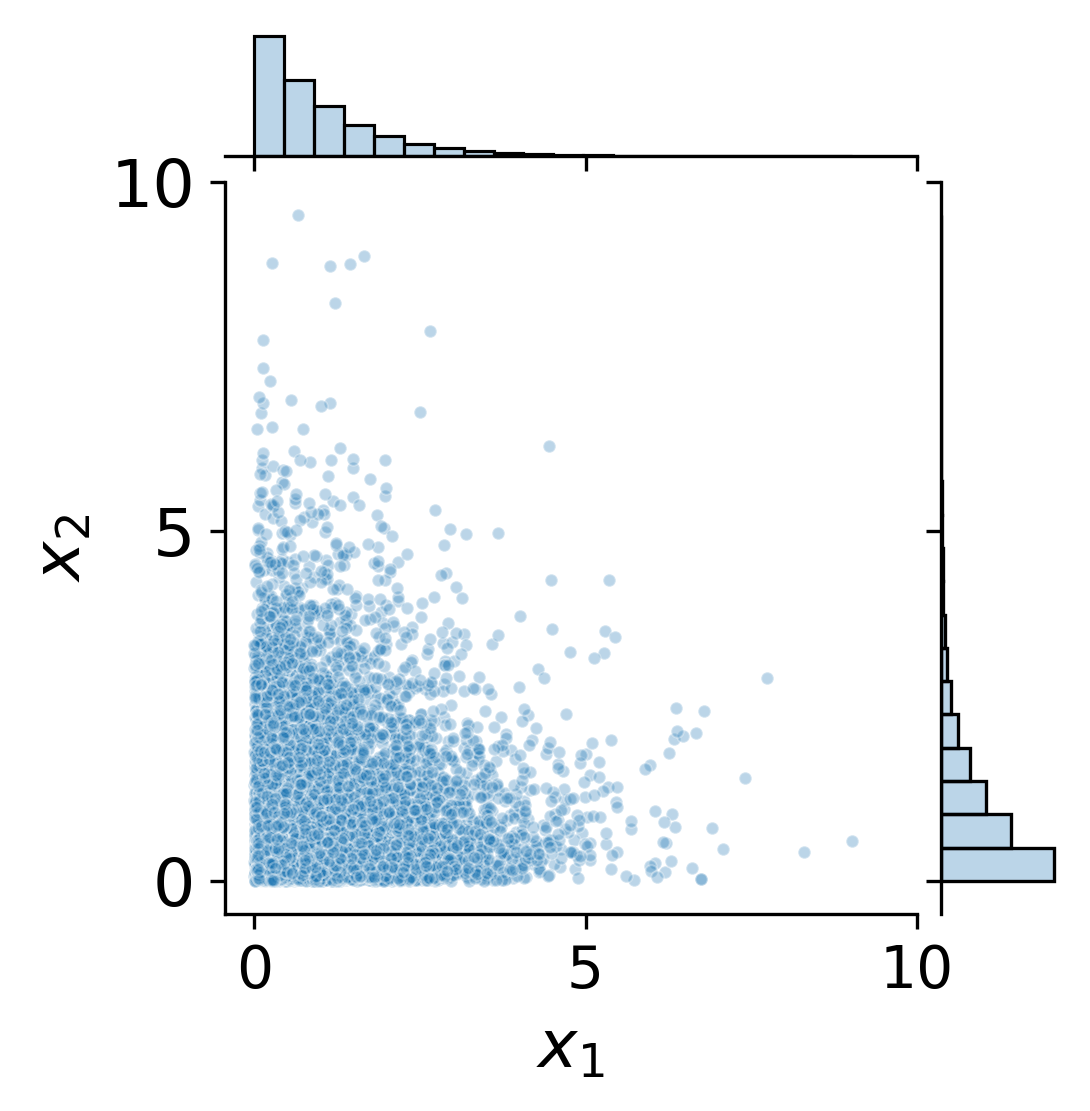
\includegraphics[width=\textwidth]{../numerical_experiments/chapter1/figures/independent_copula.png}
        \caption{Independent copula.}
    \end{subfigure}
    \hfill
    \begin{subfigure}[b]{0.32\textwidth}
        \centering
        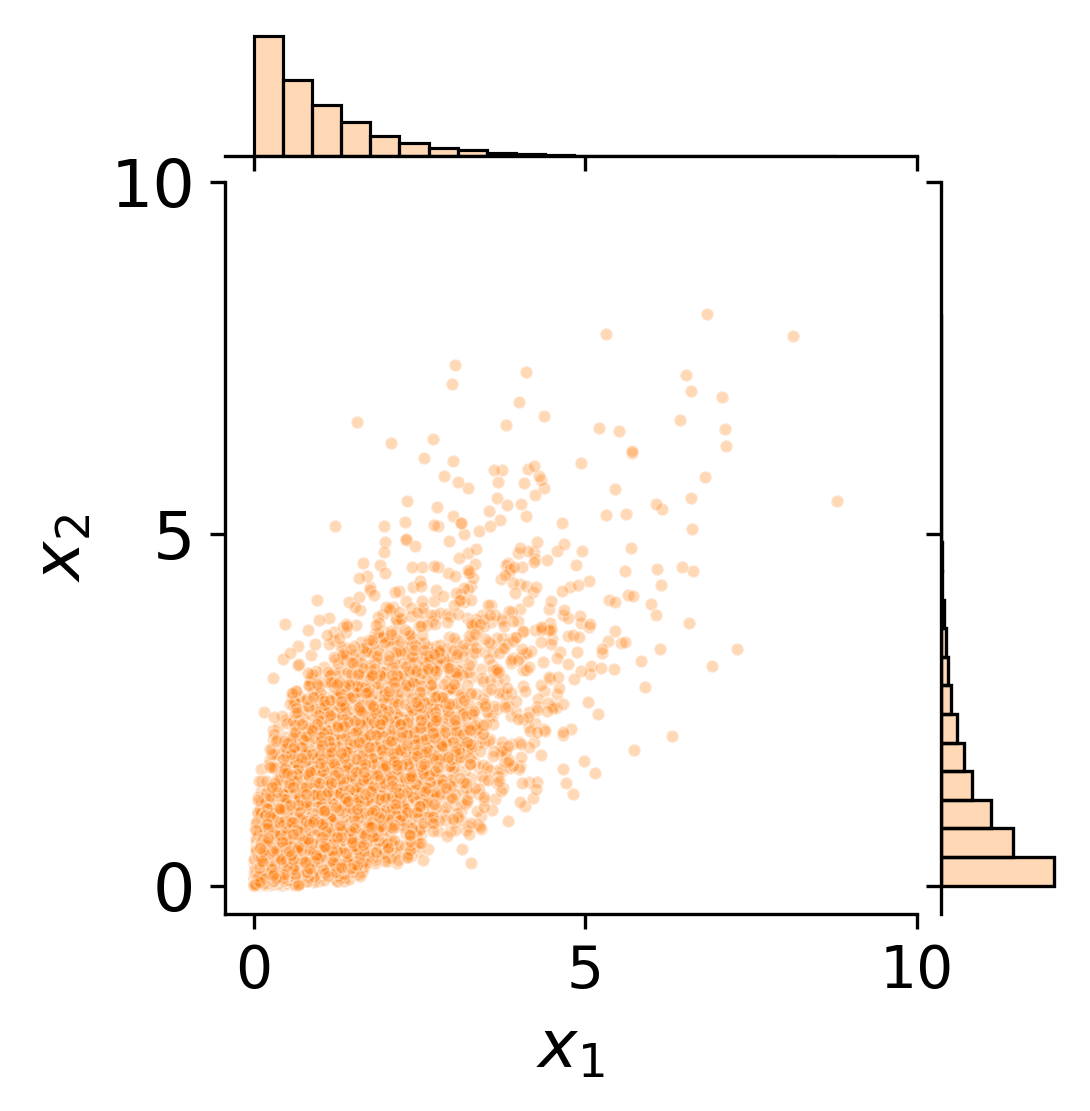
\includegraphics[width=\textwidth]{../numerical_experiments/chapter1/figures/normal_copula.png}
        \caption{Normal copula.}
    \end{subfigure}
    \hfill
    \begin{subfigure}[b]{0.32\textwidth}
        \centering
        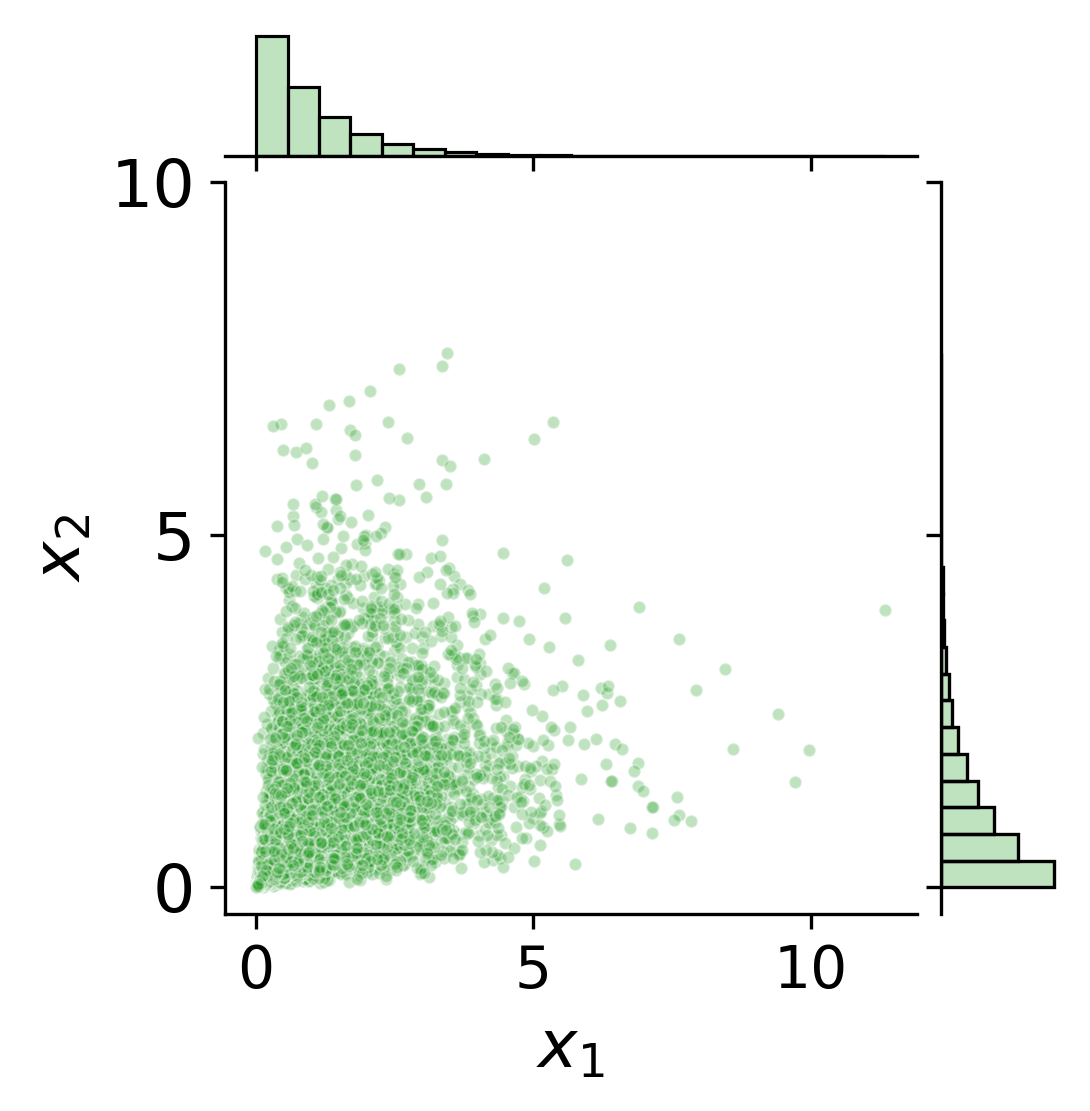
\includegraphics[width=\textwidth]{../numerical_experiments/chapter1/figures/clayton_copula.png}
        \caption{Clayton copula.}
    \end{subfigure}
       \caption{Samples of three joint distributions with identical marginals and different dependence structures.}
       \label{fig:joint_dist_samples}
\end{figure}

An empirical way of isolating the dependence structures from this example is to transform the samples in the ranked space. 
Let us consider an $n$-sized sample $\bX_n = \left\{\bx^{(1)}, \dots, \bx^{(n)}\right\} \in \iD_{\bx}^{n}$. 
The corresponding ranked sample is defined as: $\bR_n = \left\{\br^{(1)}, \dots, \br^{(n)}\right\}$, 
where\footnote{The \textit{indicator function} is defined such that $\1_{\left\{\mathcal{F}\right\}}(x) = 1$ if $x \in \mathcal{F}$ and is equal to zero otherwise.} 
$r^{(i)}_j = \sum_{l=1}^n \1_{\left\{x^{(l)}_j \leq x^{(i)}_j\right\}},$ $\forall j \in \{1, \dots d\}, i \in \{1, \dots n\}$. 
Ranking a multivariate dataset allows us to isolate the dependence structure witnessed empirically \citep{saporta_2006}. 
\fig{fig:ranked_joint_dist_samples} shows the same three samples from \fig{fig:joint_dist_samples} in the ranked space. 
One can first notice that the marginals are uniform since each rank is uniformly distributed. 
Then, the scatter plot from the distribution with independent copula (left plot) is uniform over the whole space while the others present dependence patterns. 
\begin{figure}
    \centering
    \begin{subfigure}[b]{0.32\textwidth}
        \centering
        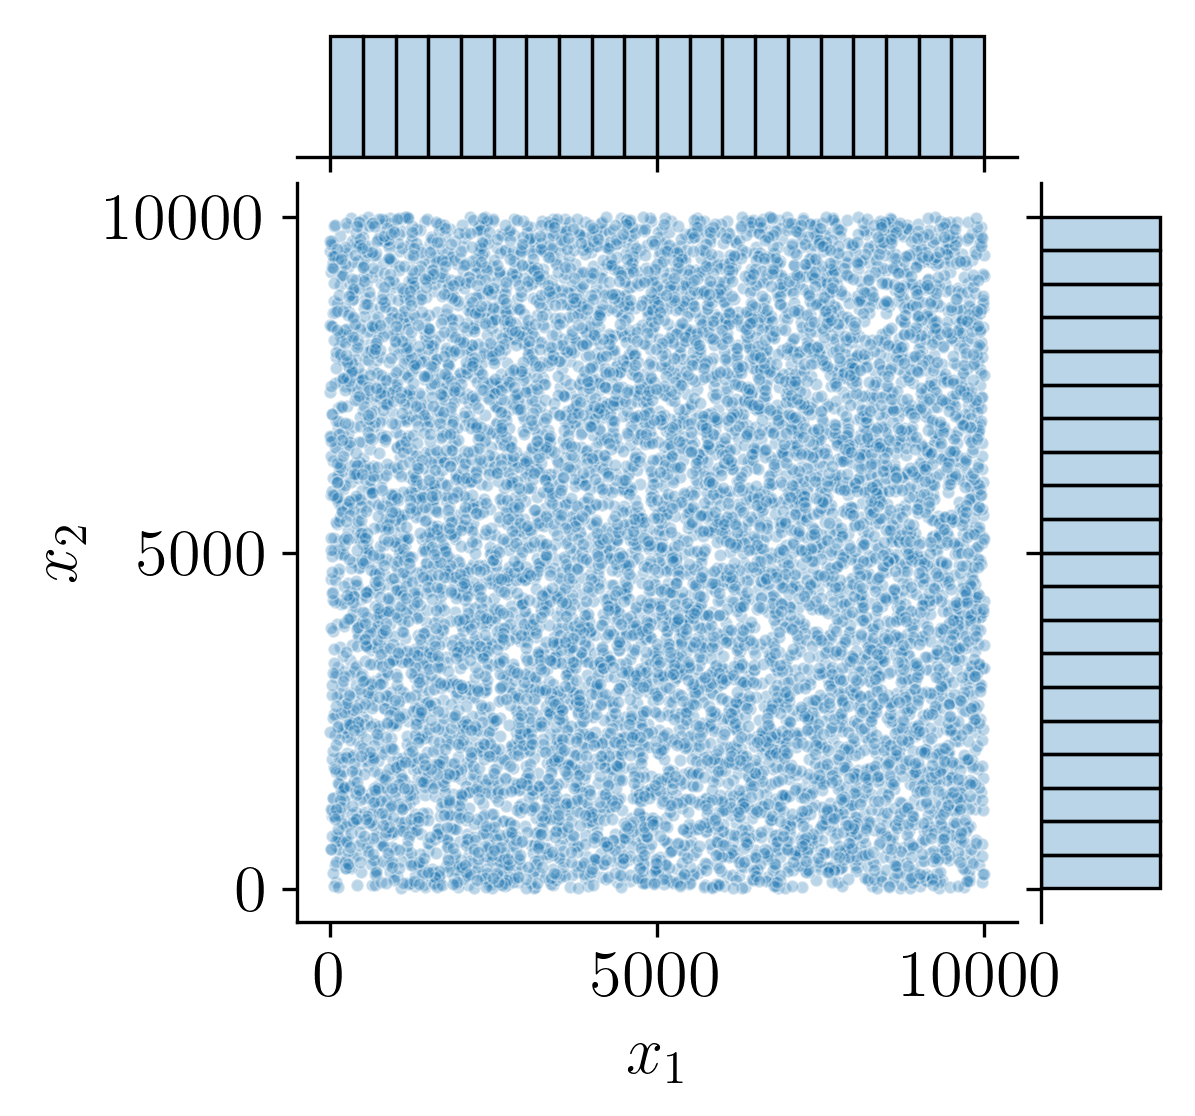
\includegraphics[width=\textwidth]{../numerical_experiments/chapter1/figures/independent_copula_ranked.png}
        \caption{Independent copula.}
    \end{subfigure}
    \hfill
    \begin{subfigure}[b]{0.32\textwidth}
        \centering
        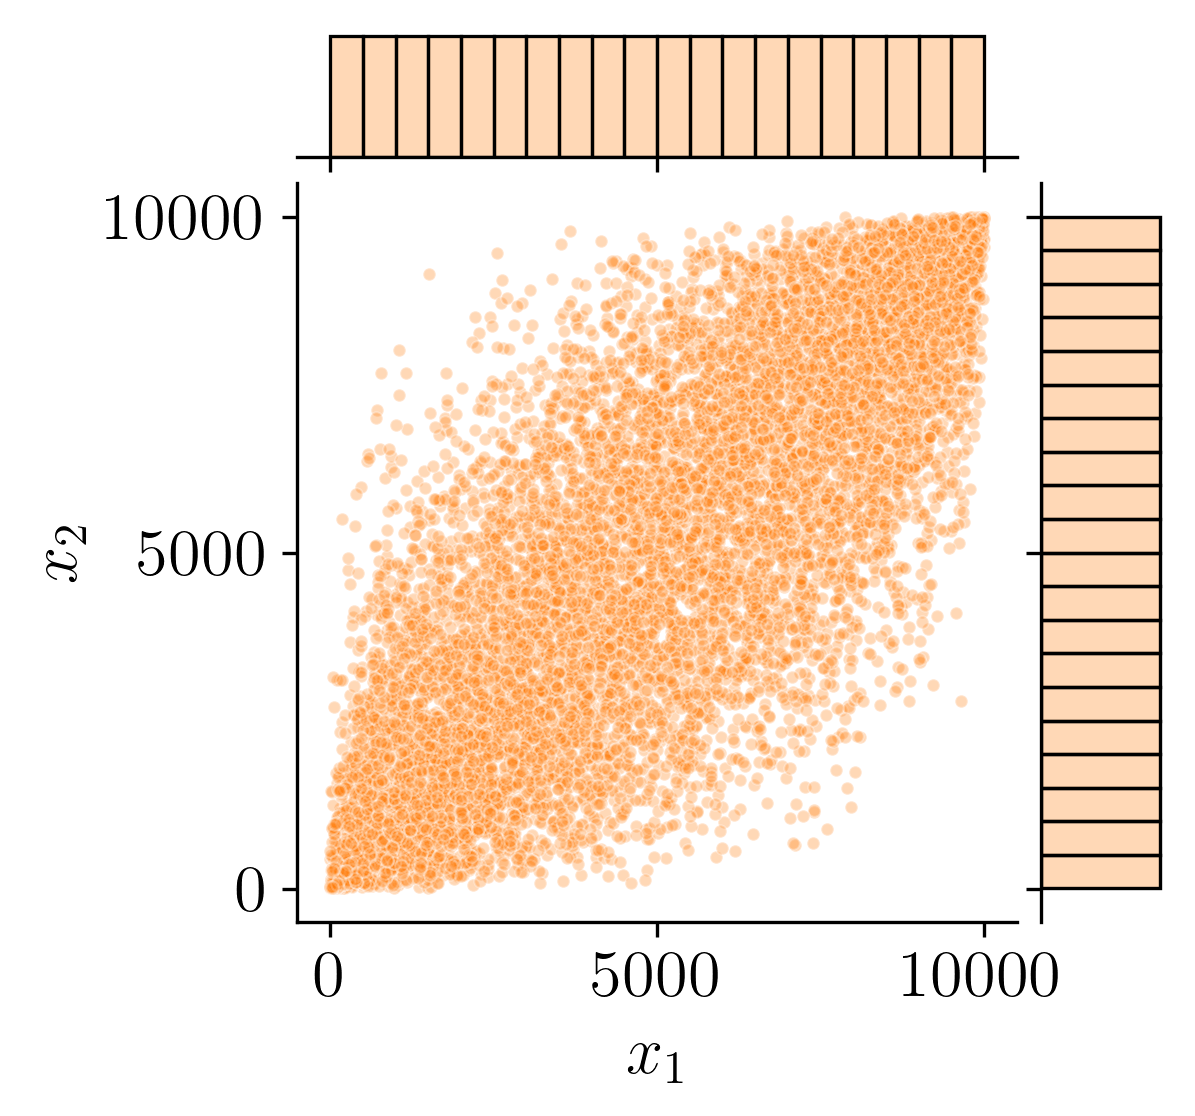
\includegraphics[width=\textwidth]{../numerical_experiments/chapter1/figures/normal_copula_ranked.png}
        \caption{Normal copula.}
    \end{subfigure}
    \hfill
    \begin{subfigure}[b]{0.32\textwidth}
        \centering
        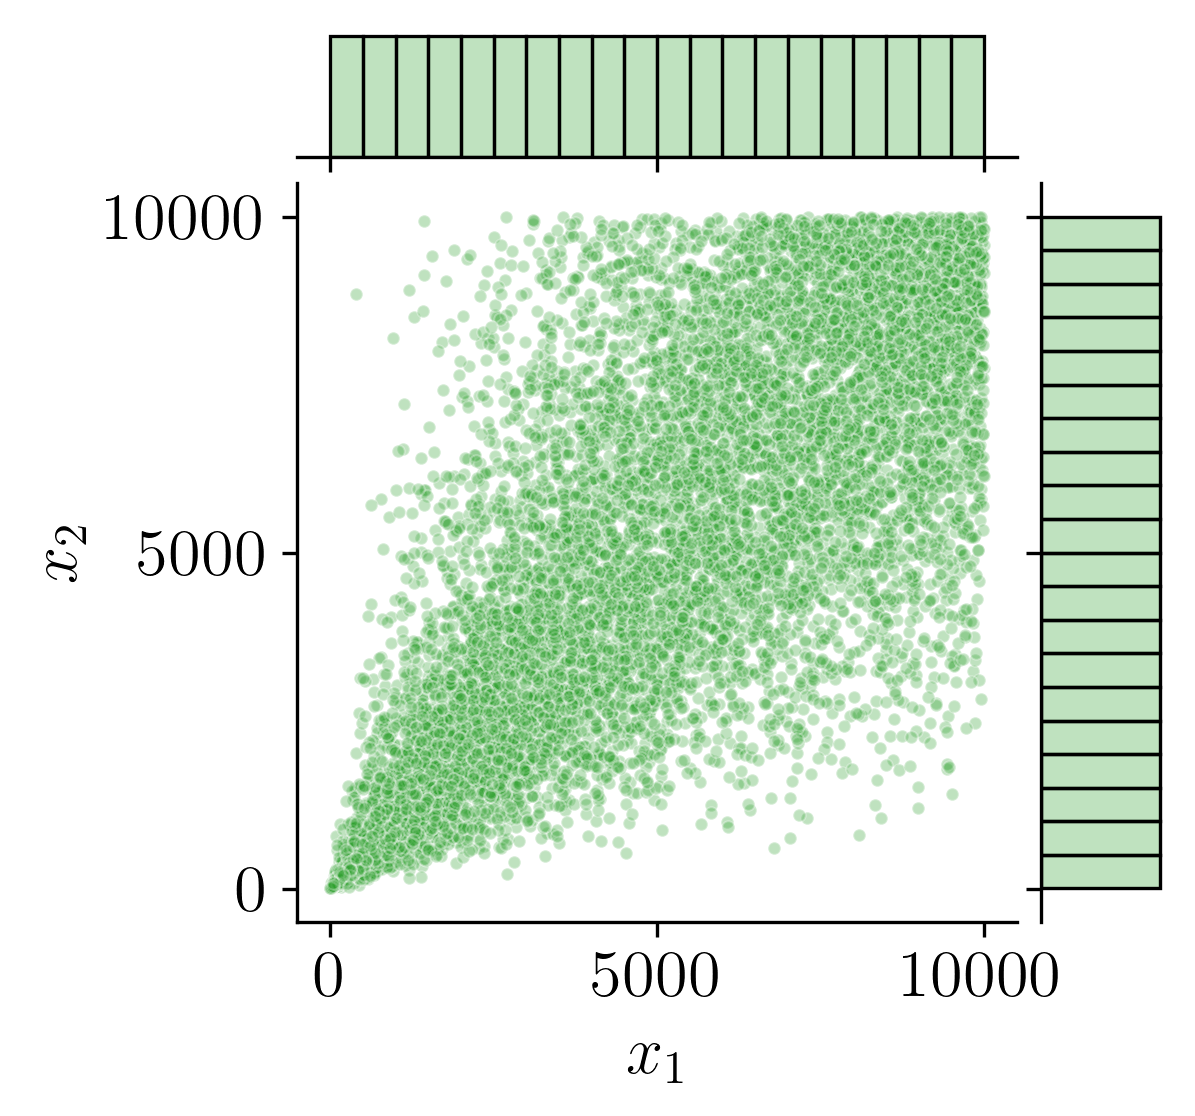
\includegraphics[width=\textwidth]{../numerical_experiments/chapter1/figures/clayton_copula_ranked.png}
        \caption{Clayton copula.}
    \end{subfigure}
       \caption{Samples in the ranked space represented in the \fig{fig:joint_dist_samples}.}
       \label{fig:ranked_joint_dist_samples}
\end{figure}

Sklar's theorem \citep{sklar_1959} states that the multivariate distribution of any random vector can be broken down into two objects. 
First, a set of univariate marginal distributions describing the behavior of each variable; 
second, a function describing the dependence structure between all variables: this function is called \textit{copula}. 

\begin{theorem}[Sklar's theorem, \citealp{sklar_1959}]
    Let $\mathbf{X} \in \R^d$ be a random vector and its joint CDF $F_{\bX}$ with marginals $\{F_{X_j}\}_{j=1}^d$. There exists a funtion $C: [0, 1]^d \rightarrow [0, 1]$, such that:
    \begin{equation}
        F_{\bX}(x_1, \dots, x_d) = \P\left(X_1\leq x_1,\dots ,X_d\leq x_d\right) = C\left(F_{X_1}(x_1), \dots, F_{X_d}(x_d)\right)\,, 
    \end{equation}
    called the ``copula''. 
    If the marginals $F_{X_i}$ are continuous, then this copula is unique. 
    If the multivariate distribution admits a PDF $f_{\bX}$, it can also be expressed as follows:
    \begin{equation}
        f_{\bX}(x_1, \dots, x_d) = c\left(F_{X_1}(x_1), \dots, F_{X_d}(x_d)\right) \times f_{X_1}(x_1) \times \dots \times f_{X_d}(x_d) \,,
    \end{equation}
    where $c$ is the density of the copula, sometimes also called ``copula'' by abuse of terminology. 
    \label{thm:sklar}
\end{theorem}

The reader might refer to \citet[Chap. 2]{durante_2015_copula} for three different mathematical proofs of this result. 
Theorem \ref{thm:sklar} expresses the joint CDF by combining marginal CDFs and a copula, which is practical for sampling joint distributions. 
Conversely, the copula can be defined by using the joint CDF and the marginal CDFs: 
\begin{equation}
    C(u_1, \dots, u_d) = F_{\bX}\left(F^{-1}_{X_1}(u_1), \dots, F^{-1}_{X_d}(u_d)\right) \,.
\end{equation}
This equation allows us to extract a copula from a joint distribution by knowing its marginals.
Additionally, copulas are invariant under increasing transformations. 
This property is essential to understand the use of rank transformation to display the copula without the marginal effects.     

Identically to the univariate continuous distributions, a large catalog of families of parametric copulas exists (independent, Normal, Clayton, Frank, Gumbel copula, etc.). 
Note that the independent copula $\Pi$ implies that the distribution is defined as the product of its marginals $\Pi = \prod_{j=1}^d u_j$. 
In an inference context, this theorem divides the fitting problem into two independent problems: fitting the marginals and fitting the copula. 
Provided a dataset, this framework allows the potential combination of a parametric (or nonparametric) fit of marginals with a parametric (or nonparametric) fit of the copula. 

To infer a joint distribution over a dataset, the analyst should determine a fitting strategy. 
Appropriate data visualization helps to choose the fitting methods susceptible to be relevant to the problem. 
In practice, the following points can be asked at this early stage:
\begin{itemize}
    \item Is the distribution unimodal? If not, mixture methods or nonparametric models might be required;
    \item Is the support restrictive? If so, specific families of parametric distributions with restrictive support can be chosen or truncation can be applied;
    \item Is there a dependence structure among the input variables? Does it concern all the variables together or only some groups of variables? 
    \item Is the dependence structure complex (e.g., stronger dependence in the tail of the distribution)? Transforming the dataset in the ranked space gives an empirical description of the dependence. 
\end{itemize} 

Techniques designed to estimate marginal distributions are available in Appendix~\ref{apx:A}. 
In addition, a nonparametric method is introduced in Chapter \ref{chpt:3} to infer a copula: the ``empirical Bernstein copula''. 
The adequation between a fitted probabilistic model and a dataset should be validated, therefore Appendix~\ref{apx:A} lists visual and quantitative tools for univariate goodness-if-fit evaluation.


%%%%%%%%%%%%%%%%%%%%%%%%%%%%%%%%%%%%%%%%%%%%%%%%%%%%%%%%%%%%%%
\begin{otexample}[\href{https://github.com/efekhari27/thesis/blob/main/numerical_experiments/chapter1/copulas.ipynb}{Bivariate distribution}]
    A minimal working example in Python is available in Appendix~\ref{apx:D}. 
    Figures illustrating the present section may be reproduced, using the \ots scripts available on the GitHub repository\footnotemark. 
\end{otexample}
%%%%%%%%%%%%%%%%%%%%%%%%%%%%%%%%%%%%%%%%%%%%%%%%%%%%%%%%%%%%%%
\footnotetext{\url{https://github.com/efekhari27/thesis/blob/main/numerical_experiments/chapter1/copulas.ipynb}}

%============================================================%
%============================================================%
\section{Uncertainty propagation for central tendency study} \label{sec:central_propagation}
%============================================================%
%============================================================%
The previous section aimed at building a probabilistic model of the uncertainties considering the available knowledge. 
This one introduces diverse methods for forward propagation of the input uncertainties through a numerical model. 
In the present section, uncertainty propagation is dedicated to the ``central tendency'' as its goal is to study the mean and variance of the output distribution. 
This approach contrasts with the uncertainty propagation committed to rare event probability estimation, which will be introduced in Section~\ref{sec:reliability} (e.g., used to assess reliability). 

The difficulties related to any uncertainty propagation task mostly arise from the practical properties of the numerical model. 
Its potential high dimension, irregularity and nonlinearity each represent a challenge. 
Such studies rely on a finite number of observations of the numerical model, depending on the computational affordable budget.  
Uncertainty propagation is at the end of the generic UQ approach (step C), however, it is affected by the ``garbage in, garbage out'' concept. 
Meaning that its conclusions depend on the accuracy of the inputs' uncertainty modeling. 

This section introduces the main methods of uncertainty propagation for central tendency estimation, 
outlining the links between numerical integration and the numerical design of experiments. 


%============================================================%
\subsection{Numerical integration}
%============================================================%
Forward uncertainty propagation aims at integrating a measurable function $g: \iD_{\bX} \rightarrow \R$ w.r.t. a probability measure $\P_{\bX}$. 
Numerical integration provides algorithmic tools to help the resolution of this probabilistic integration problem. 
To ease the notations, the numerical model $\iM(\cdot)$ introduced in \eq{eq:numerical_model} is replaced by a generic measurable function $g(\cdot)$.
%Note that the measurable function $g$, in the context of computer experiments, becomes the numerical model $\iM$ introduced in \eq{eq:numerical_model}. 

In practice, this integral is approximated by summing a finite $n$-sized set of realizations $\by_n = \left\{g(\bx^{(1)}), \dots, g(\bx^{(n)})\right\}$ from a set of input samples $\bX_n = \left\{\bx^{(1)}, \dots, \bx^{(n)}\right\}$. 
A \textit{quadrature} selects the input samples $\bX_n$ (also called ``nodes'' in classical numerical integration), and an associated set of weights $\bw_n = \{w_1, \dots, w_n\} \in \R^n$. 
The approximation given by a quadrature rule is defined as a weighted arithmetic mean of the realizations:
\begin{equation}
    I_{\P_{\bX}}(g) = \E[g(\bX)] = \int_{\iD_\bX} g(\bx) \, \dd\P_{\bX}(\bx) \approx \sum_{i=1}^n w_i \, g\left(\bx^{(i)}\right).
    %\label{eq:quadrature_rule}
\end{equation}
For a given sample size $n$, the goal is to find a set of tuples $\left\{\bx^{(i)}, w_i \right\}_{i=1}^n$ (i.e., a quadrature rule), which provide the best approximation of the quantity of interest $I_{\P_{\bX}}(g)$. 
Ideally, the approximation quality should be fulfilled for a wide class of integrands (e.g., regardless of their regularity). 
Most quadrature rules only depend on the probability space $(\Omega, \iA, \P_{\bX})$, regardless of the integrand values. 
In the context of a costly numerical model, defining the quadrature ahead allows the analyst to massively distribute the evaluations of the numerical model. 

%This section aims to present the main multivariate integration techniques. 
%These methods encompass different properties: 
%some are deterministic and some are aleatory; 
%some are sequential (i.e., nested) some are not; 
%some are victims of the curse of dimensionality and some are not. 

%\item Some quadratures define negative weights, which can introduce numerical instabilities when $n$ gets large.
%\item The nature of the probability measure (i.e., presence of dependence) might restrict the use of methods

%------------------------------------------------------------%
\subsubsection{Classical multivariate deterministic quadrature}
%------------------------------------------------------------%

Historically, quadrature methods have been developed for univariate integrals. 
The Gaussian rule and the Fej\'{e}r-Clenshaw-Curtis rule are two univariate deterministic quadratures that will be briefly introduced (see \citealp{sullivan_2015} for further elements). 

%Let us first mention the Newton-Cotes quadratures, generalizing multiple rules (e.g., the trapezoidal rule, Simpson's rule, etc.).
Gaussian quadrature is a powerful univariate quadrature building together a set of irregular nodes and a set of weights. 
The computed weights are positive, which ensures a numerically stable rule even for large sample sizes.
Different variants of Gaussian rules exist, the most common one being the Gauss-Legendre quadrature. 
In this case, the function $g$ to be integrated w.r.t. the uniform measure on $[-1, 1]$ is approximated by Legendre polynomials. 
Considering the Legendre polynomial of order $n$, denoted $l_n$, the quadrature nodes $\{x^{(i)}\}_{i=1}^n$ are given by the polynomial roots, while the respective weights are given by the following formula: 
\begin{equation}
    w_{i}={\frac {2}{\left(1-\left(x^{(i)}\right)^{2}\right)\left(l'_{n}(x^{(i)})\right)^{2}}}.
\end{equation}
Gauss-Legendre quadrature guarantees a very precise approximation provided that the integrand is well-approximated by a polynomial of degree $2n-1$ or less on $[-1, 1]$.
This rule is deterministic but not sequential, meaning that two rules with sizes $n_1$ and $n_2$, $n_1 < n_2$ will not be nested (i.e., its construction is not iterative). 
However, a sequential extension is proposed by the Gauss-Kronrod rule \citep{laurie_1997}, at the expense of a slightly lower accuracy regarding $I_{\P_{\bX}}(g)$. 

To overcome this practical drawback, Fej\'{e}r \citep{fejer_1933} then Clenshaw and Curtis \citep{clenshaw_1960} proposed a nested rule with mostly equivalent accuracy as Gaussian quadratures.
This method is usually presented to integrate a function w.r.t. the uniform measure on $[-1, 1]$ and starts with a change of variables, $x:=\cos(\theta), \, \dd x := \sin(\theta)$:
\begin{equation}
    \int_{-1}^{1} g(x) \, \dd x = \int_{0}^{\pi} g\left(\cos(\theta)\right) \, \sin(\theta) \, \dd \theta. 
\end{equation}
This expression can be written as an expansion of the integrand using trigonometric series. 
Therefore, knowing that cosine series are closely related to the Chebyshev polynomials of the first kind, 
Fej\'{e}r's ``first rule'' \citep{trefethen_2008} uses the Chebyshev polynomials roots as nodes $x^{(i)} = \cos(\theta^{(i+1/2)})$, associated with the following weights:
\begin{equation}
    w_i=\frac{2}{n}\left(1-2\sum_{j=1}^{\lfloor n/2 \rfloor}\frac{1}{4j^2-1}\cos\left(j\theta^{(2i+1)}\right)\right),    
\end{equation}
where $\lfloor \cdot \rfloor$ denotes the floor function. 

These two univariate integration schemes are both very efficient on a wide panel of functions. 
Yet, Fej\'{e}r-Clenshaw-Curtis is sequential and offers easy implementations, benefitting from powerful algorithms such as the fast Fourier transform. 
\fig{fig:univariate_quads} illustrates the nested properties of Fej\'{e}r-Clenshaw-Curtis quadrature by representing the nodes of quadrature rules with increasing size on the y-axis.  
For example, the Fej\'{e}r-Clenshaw-Curtis quadrature with size $n=13$ includes all the nodes from the quadratures with sizes $n=7$ and $n=4$. 

\begin{figure}[ht]
    \centering
    \begin{subfigure}[b]{0.32\textwidth}
        \centering
        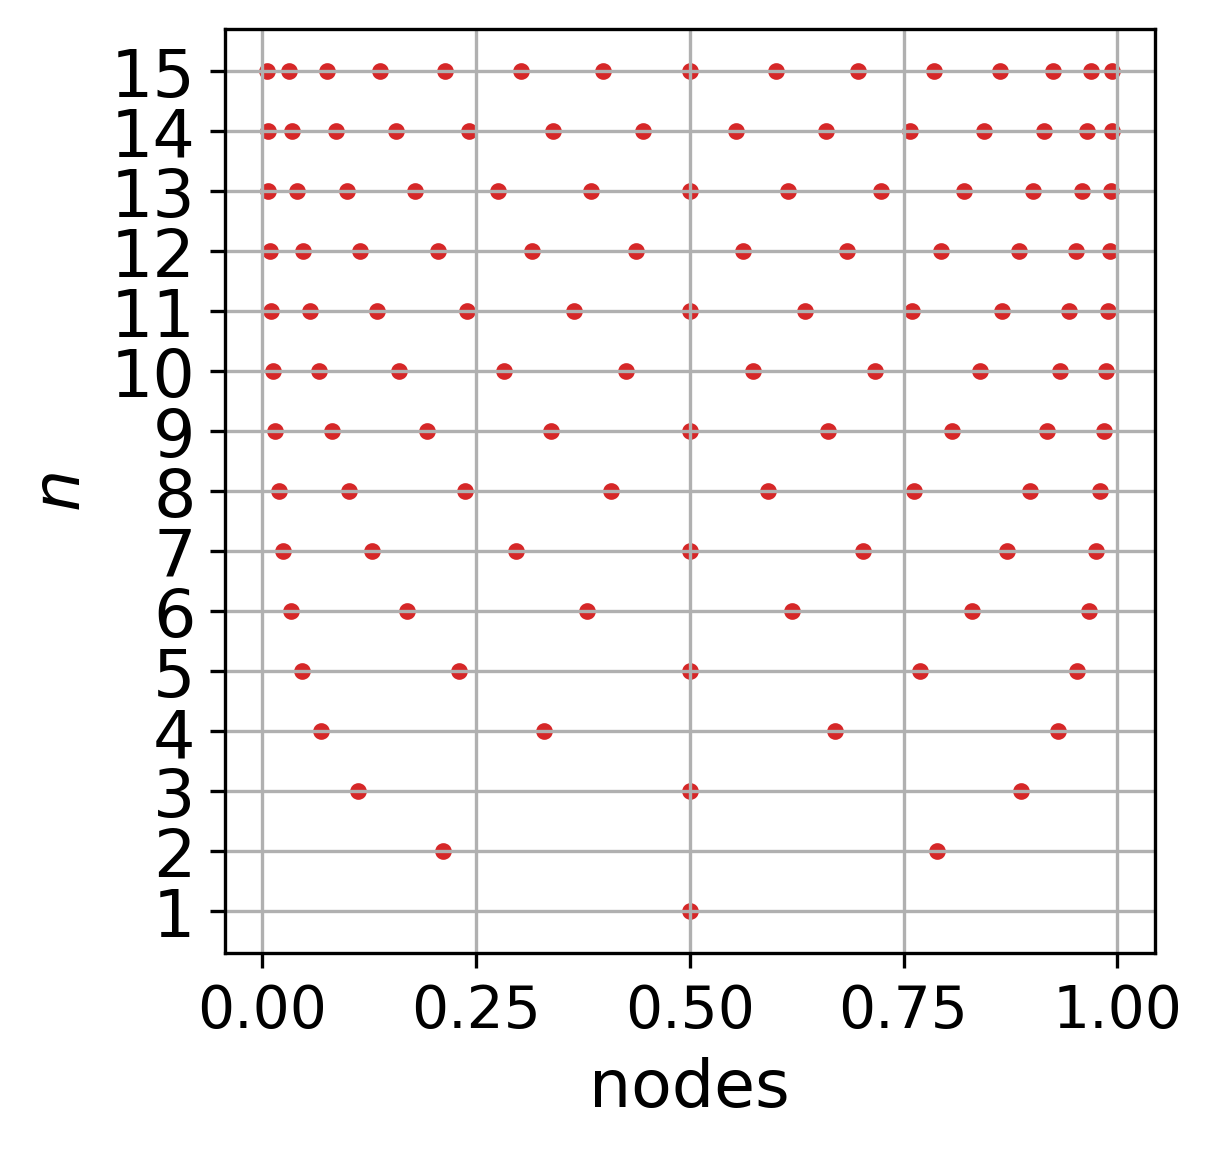
\includegraphics[width=\textwidth]{../numerical_experiments/chapter1/figures/univariate_gauss_legendre.png}
        \caption{Gauss-Legendre.}
    \end{subfigure}
    \quad
    \begin{subfigure}[b]{0.32\textwidth}
        \centering
        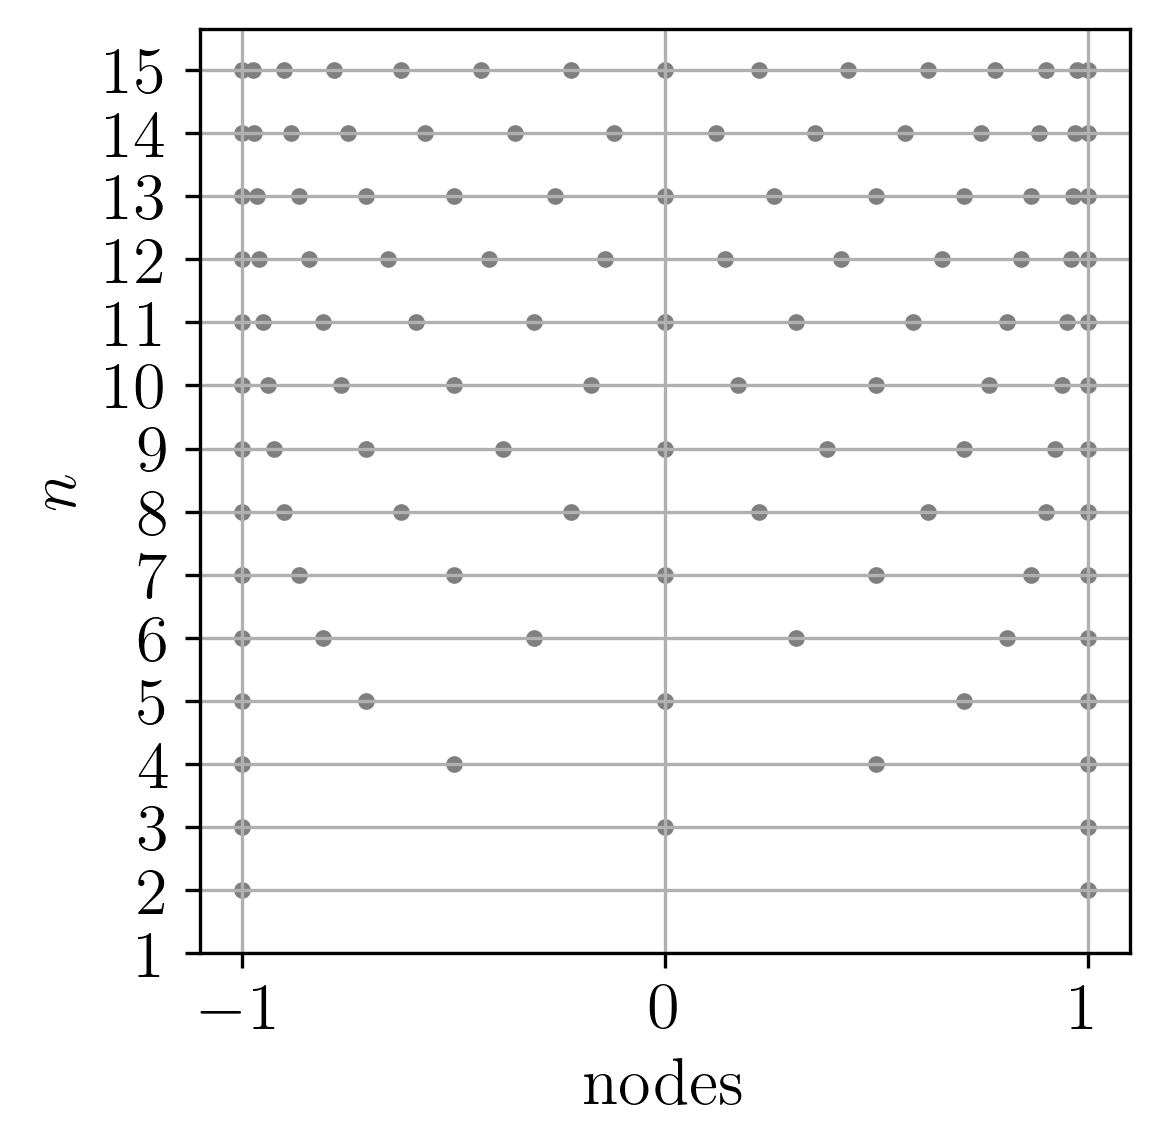
\includegraphics[width=\textwidth]{../numerical_experiments/chapter1/figures/univariate_clenshaw_curtis.png}
        \caption{Clenshaw-Curtis.}
    \end{subfigure}
    \caption{Univariate quadratures nodes for increasing sizes ($1 \leq n \leq 15$).}
    \label{fig:univariate_quads}
\end{figure}


However, in practice, UQ problems are rarely unidimensional, but one can directly extend these univariate rules to multivariate ones by defining the tensor product (also called ``full grids'') of univariate rules. 
This exhaustive approach quickly shows its practical limits as the problem's dimension increases. 
In \fig{fig:bivariate_quads}, the left plot represents a two-dimensional tensor product of identical Gauss-Legendre quadratures. 
Alternatively, sparse multivariate quadratures (i.e., Smolyak sparse grid) explore the joint domain more efficiently. 
Using the Smolyak recurrent formula (see e.g., \citealp{sullivan_2015}), two univariate quadratures can be combined as illustrated on the right of \fig{fig:bivariate_quads}. 
Finally, this technique showed great properties, but other methods offer more flexibility and guarantees.

\begin{figure}[h!]
    \centering
    \begin{subfigure}[b]{0.32\textwidth}
        \centering
        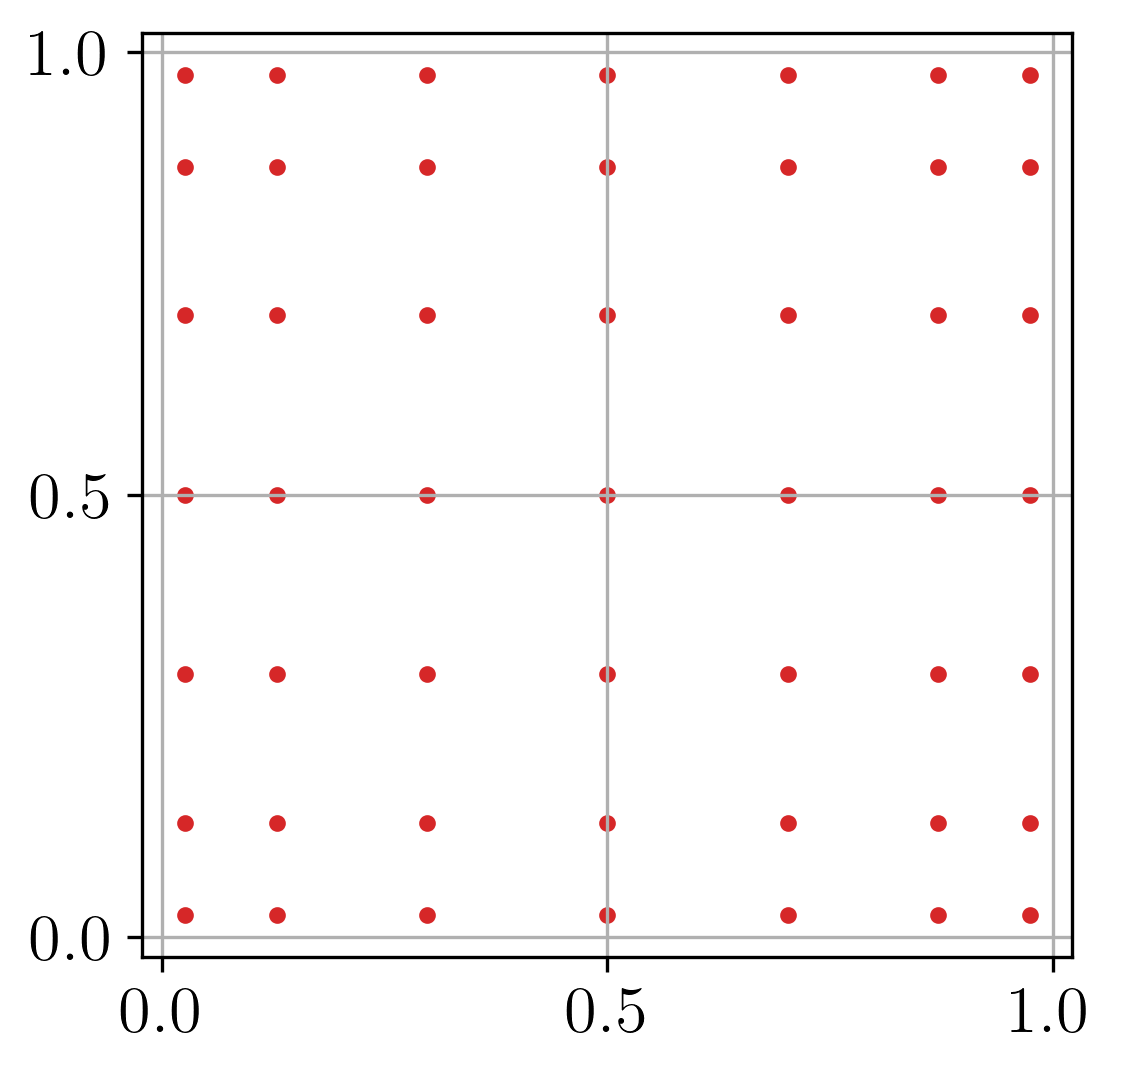
\includegraphics[width=\textwidth]{../numerical_experiments/chapter1/figures/tensorized_gaussian_quadrature.png}
        \caption{Tensor product (n=49).}
    \end{subfigure}
    \quad
    \begin{subfigure}[b]{0.32\textwidth}
        \centering
        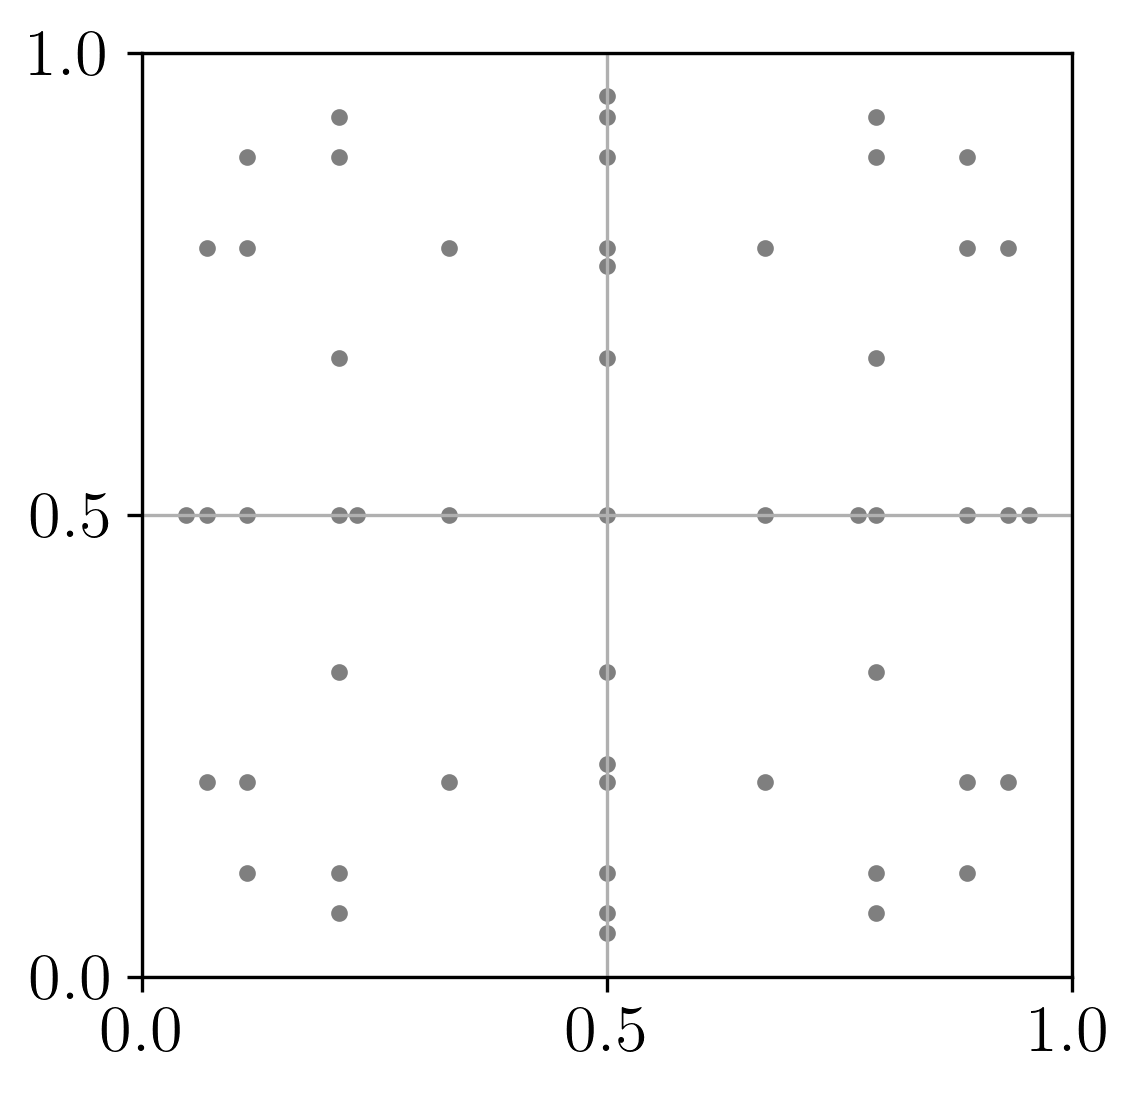
\includegraphics[width=\textwidth]{../numerical_experiments/chapter1/figures/smolyak_gaussian_quadrature.png}
        \caption{Smolyak sparse grid (n=53).}
    \end{subfigure}
    \caption{Two identical univariate Gauss-Legendre quadratures combined as a tensor product (left) and a Smolyak sparse grid (right).}
    \label{fig:bivariate_quads}
\end{figure}


%------------------------------------------------------------%
\subsubsection{Monte Carlo methods}
%------------------------------------------------------------%
Monte Carlo methods were initially developed in the 1940s to solve problems in neutronics.  
Ever since, this technique has been applied to the numerical resolution of integrals. 
To integrate a function $g$ against a measure $\P_{\bX}$, it randomly generates points according to the input measure. 
The integral is estimated by taking the uniform arithmetic mean of the nodes' images obtained. 

This method requires to be able to generate points following a given distribution. 
To do so, the most common approach is to first uniformly generate a sequence of random points on $[0, 1]$. 
These sequences mimic actual randomness but are in fact generated by deterministic algorithms, also called pseudorandom number generators. 
Pseudorandom algorithms generate a sequence of numbers with a very large, but finite length. 
This sequence can be exactly repeated by fixing the same initial point, also called \textit{pseudorandom seed}.
Most programming languages use the Mersenne-Twister pseudorandom generator \citep{matsumoto_1998}, offering a very long period (around $4.3\times10^{6001}$ iterations).

Formally, the ``Vanilla'' Monte Carlo (sometimes called ``crude'' Monte Carlo) method uses a set of i.i.d. samples $\bX_n = \left\{\bx^{(1)}, \dots, \bx^{(n)}\right\} \sim \P_{\bX}$. 
The Monte Carlo estimator of the integral is given by: 
\begin{equation}
    I_{\P_{\bX}}(g) \approx \overline{y}_n^{\textrm{MC}} = \frac1n \sum_{i=1}^{n} g(\bx^{(i)}).
\end{equation}
By construction, the strong law of large numbers makes this estimator unbiased and strongly consistent. 
However, it converges relatively slowly. 
The variance of the Monte Carlo estimator results from a manipulation of the central limit theorem:
\begin{equation}
    \var\left(\overline{y}_n^{\textrm{MC}}\right) = \frac{1}{n} \var\left(Y\right). 
    \label{eq:MC_variance}
\end{equation}
Considering the images of the sample $\bX_n$, one can also express the unbiased empirical variance of the output random variable $\what{\sigma}^2_Y = \frac{1}{n-1} \sum_{i=1}^n \left(g(\bx^{(i)}) - \overline{y}_n^{\textrm{MC}}\right)^2$.
The Monte Carlo estimator also comes with theoretical confidence intervals at $\alpha \%$, given for a known value of $\var(g(\bX))$ by: 
\begin{equation}
    I_{\P_{\bX}}(g) \in \left[\overline{y}_n^{\textrm{MC}}  - q_\alpha \sqrt{\frac{\var\left(g(\bX)\right)}{n}}, \, \overline{y}_n^{\textrm{MC}}  + q_\alpha \sqrt{\frac{\var\left(g(\bX)\right)}{n}} \right],
    \label{eq:MC_IC}
\end{equation}
where $q_\alpha = \Phi(1 - \alpha/2)$, and $\Phi$ is the CDF of the standard normal distribution. 
Monte Carlo presents the advantage of being a universal method, with no bias and strong convergence guarantees. 
Moreover, it is worth noting that its convergence properties do not explicitly depend on the dimension of the input domain. 
Unlike the previous multivariate deterministic quadrature, it does not explicitly suffer from the curse of dimensionality. 
The main limit of crude Monte Carlo is its convergence speed, making it intractable for most practical cases. 
More recent methods aim at keeping the interesting properties of this technique while making it more efficient. 
Among the \textit{variance reduction} methods, let us mention importance sampling, stratified sampling (e.g., Latin hypercube sampling), control variates and multi-level Monte Carlo. 
For further details, the reader may refer to \citet[Chap. 8,9,10]{owen_2013} and \citep{giles_2008}.


%------------------------------------------------------------%
\subsubsection{Quasi-Monte Carlo and Koksma-Hlawka inequality}\label{sec:1qmc}
%------------------------------------------------------------%

Among the methods presented so far, classical deterministic quadratures are subject to the curse of dimensionality while Monte Carlo methods deliver mixed performances. 
Quasi-Monte Carlo (\abv{qmc}) is a deterministic family of numerical integration schemes w.r.t. the uniform measure on $[0, 1]$. 
It offers powerful performances with strong guarantees by choosing nodes according to \textit{low discrepancy} sequences. 
The discrepancy of a set of nodes (or a design) can be seen as a metric of its uniformity. 
The lower the discrepancy of a design is, the ``closest'' it is to uniformity. 

The Koksma-Hlawka inequality given in Theorem~\ref{thm:koksma_inequality} \citep{morokoff_1995,leobacher_2014} is a fundamental result for understanding the role of the discrepancy in numerical integration. 
\begin{theorem}[Koksma-Hlawka inequality]\label{thm:koksma_inequality}
    If $g:[0, 1]^d\rightarrow\R$ has a bounded variation (i.e., its variation is finite), then for any design $\bX_n = \left\{\bx^{(1)}, \dots, \bx^{(n)}\right\} \in [0, 1]^d$:
    \begin{equation}
        \left| \int_{[0, 1]^d} g(\bx) \ddx - \frac1n \sum_{i=1}^n g\left(\bx^{(i)}\right)\right| \leq  V(g) D^*(\bX_n),
    \end{equation}
    where $D^*(\bX_n)$ is the star discrepancy of the design $\bX_n$, while $V(g)$ quantifies the complexity of the integrand, which is related to its variation. 
\end{theorem}

The reader might refer to \citet[Sec. 3.4]{leobacher_2014} for further mathematical proof.
The function's variation $V(g)$ in Theorem~\ref{thm:koksma_inequality} can be formally defined as the Hardy-Klause variation: 
\begin{equation}
    V(g) = \sum_{\mathfrak{u}\subseteq\{1, \dots, p \}} \int_{[0, 1]^\mathfrak{u}} \left| \frac{\partial^{\mathfrak{u}}g}{\partial \bx_{\mathfrak{u}}}(\bx_{\mathfrak{u}}, 1)\right| \dd\bx.
\end{equation}
According to \citealp[p.188]{sullivan_2015}, this variation coincides with the notion of total variation defined in Appendix~\ref{apx:B} for $d=1$.

The star discrepancy $D^*(\bX_n)$ can be defined from a geometric point of view. 
Let us first consider the number of elements from a design $\bX_n$, falling in a subdomain $[\mathbf{0}, \bx)$ as $\#(\bX_n \cap [\mathbf{0}, \bx))$, where $\#$ denotes the cardinal of a set. 
Then, if this empirical quantification is compared with the volume of the rectangle $[\mathbf{0}, \bx)$, denoted by $\mathrm{vol}\left([\mathbf{0}, \bx)\right)$.
Thus, the star discrepancy is expressed as:   
\begin{equation}
    D^*(\bX_n) = \sup_{\bx \in [0, 1]^d} \left| \frac{\#(\bX_n \cap [\mathbf{0}, \bx))}{n} - \mathrm{vol}\left([\mathbf{0}, \bx)\right)\right|.
\end{equation}
The star-discrepancy $D^*(\bX_n)$ is actually a particular case of the \textit{$L_p$ star discrepancy} denoted by $D^*_p(\bX_n)$, for which $p=\infty$. 
In the general case, $D^*_p(\bX_n)$ is defined as the $L_p$-norm of the difference between the empirical CDF of the design $\what{F}_{\bX_n}$ and the CDF of the uniform distribution $F_{\textbf{U}}$:  
\begin{equation}
    D^*_p(\bX_n) = \lVert \what{F}_{\bX_n} - F_{\textbf{U}}\rVert _p = \left(\int_{[0, 1]^d} \left\lvert\what{F}_{\bX_n}(\bx) - F_{\textbf{U}}(\bx)\right\rvert ^p \, \ddx \right)^{1/p}.
\end{equation}
Interestingly, the star discrepancy $D^*(\bX_n)$ is equivalent to the Kolmogorov-Smirnov statistic, verifying whether the design follows a uniform distribution \citep{fang_liu_2018}. 

In Theorem~\ref{thm:koksma_inequality}, one can notice how the Koksma-Hlawka inequality dissociates the quadrature performance into a contribution from the function complexity and one from the repartition of the quadrature nodes. 
Knowing that the complexity of the studied integrand is fixed, this property explains the motivation to generate low-discrepancy sequences for quadrature.  

Note that the design can also be considered as a discrete distribution (uniform sum of Dirac distributions).
The discrepancy can then be expressed as a probabilistic distance between this discrete distribution and the uniform distribution. 
A generalized discrepancy between distributions called the \textit{maximum mean discrepancy} is introduced in Appendix~\ref{apx:D} and used for efficient sampling in Chapter \ref{chpt:4} of this manuscript.

Some famous low-discrepancy sequences (e.g., van der Corput, Halton, Sobol', Faure) can offer a bounded star discrepancy such that $D^*(\bX_n) \leq \frac{C \log(n)^d}{n}$, where the constant $C$ depends on the type of sequence.
Therefore, using these sequences as a quadrature rule with uniform weights provides the following absolute error upper bound: 
\begin{equation}
    \left| \int_{[0, 1]^d} g(\bx) \ddx - \frac1n \sum_{i=1}^n g\left(\bx^{(i)}\right)\right| \leq  \frac{V(g) \log(n)^d}{n}.
\end{equation}

%This bound is qualified as sharp since for any design $\bX_n$, and every $\epsilon > 0$, a function $g$ with variation $V(g)=1$ exists such that:
%\begin{equation}
%    \left| \int_{[0, 1]^d} g(\bx) \ddx - \frac1n \sum_{i=1}^n g\left(\bx^{(i)}\right)\right|  > D^*(\bX_n) - \epsilon.
%\end{equation} 

The generation of such sequences does not necessarily require more effort than pseudorandom sampling. 
In \citet[Chap. 15]{owen_2013}, an extended presentation is offered about the various ways of generating low-discrepancy sequences. 
For example, the van der Corput and Halton sequences rely on congruential generators. 
%Then, scrambling procedures are sometimes implemented to correct pathologies famously observed on Halton sequences. 

Halton sequences in medium dimension, unfortunately, introduce pathological patterns when looking at their subprojections. 
To overcome these limits, other methods such as the famous Sobol' or Faure sequences were developed (later gathered under a generic notion called ``digital nets'' by \citealp{dick_2010_digital_nets}).  
Sobol' sequences are in base two and have the advantage of being extensible in dimension. 
Note that by construction, these sequences offer particularly low discrepancies for specific size values. 
Typically, designs with sizes equal to powers of two or power of prime numbers will be favorable. 
To illustrate the different repartition and properties of the methods, \fig{fig:quasi_monte_carlo_designs} represents the three Monte Carlo and QMC designs (with size $n=2^8=256$). 
Each one is then split into the first $n_1=128$ points (in red) and the following $n_2=128$ points (in black) to show to nested properties of the QMC sequences. 
This illustration clearly shows the way QMC sequences uniformly occupy the domain while Monte Carlo sampling leaves uncovered areas.  

\begin{figure}[ht]
    \centering
    \begin{subfigure}[b]{0.32\textwidth}
        \centering
        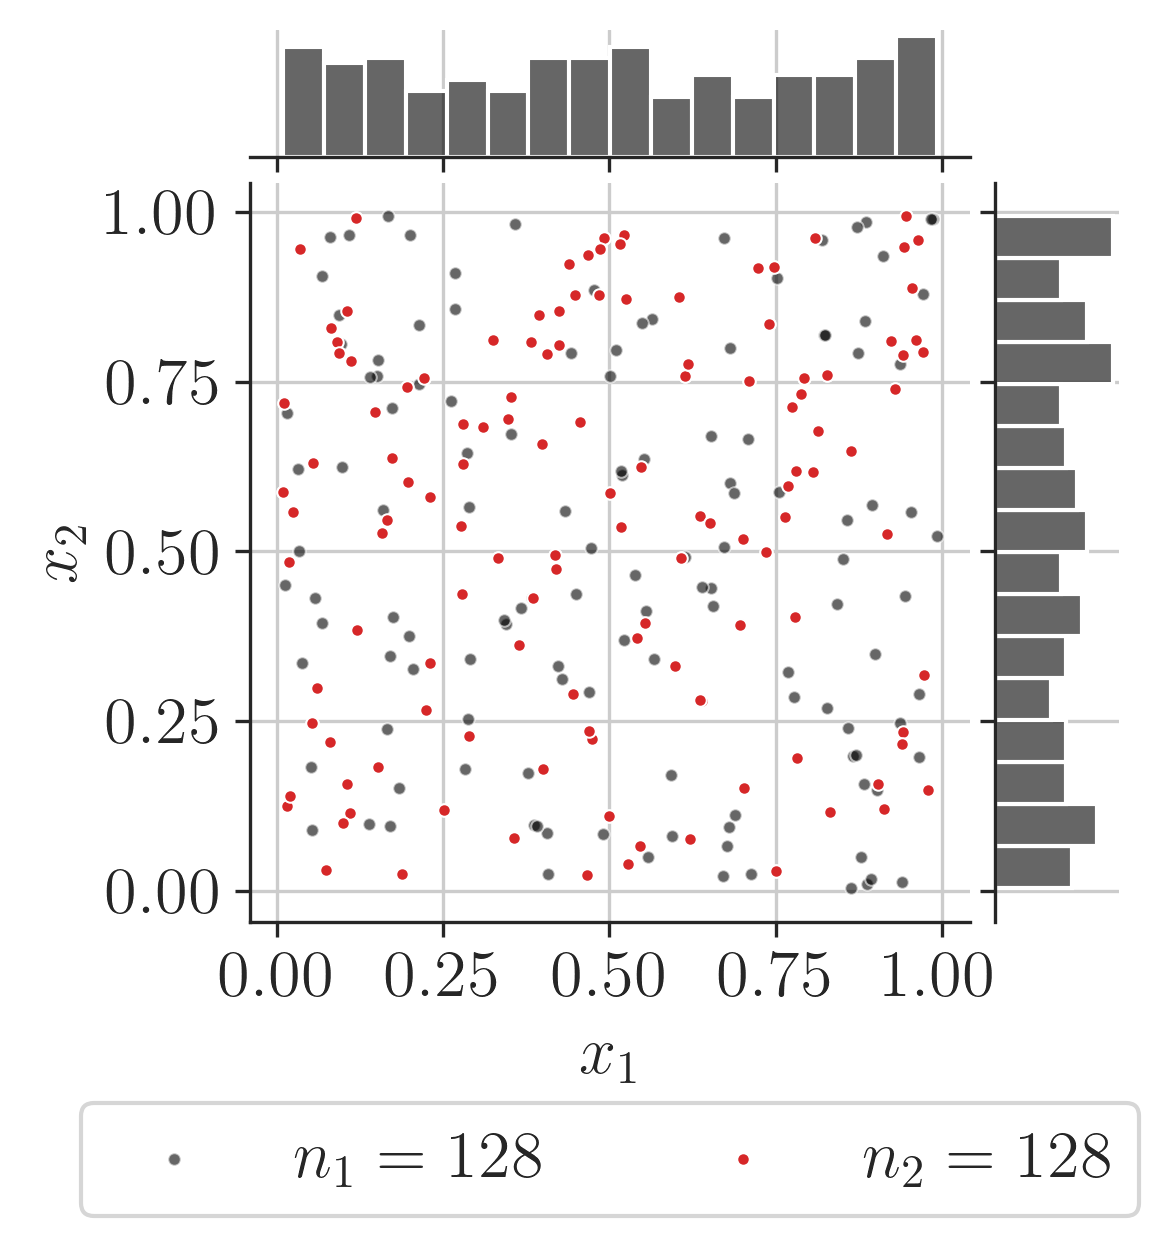
\includegraphics[width=\textwidth]{../numerical_experiments/chapter1/figures/MonteCarlo256.png}
        \caption{Monte Carlo.}
    \end{subfigure}
    \hfill
    \begin{subfigure}[b]{0.32\textwidth}
        \centering
        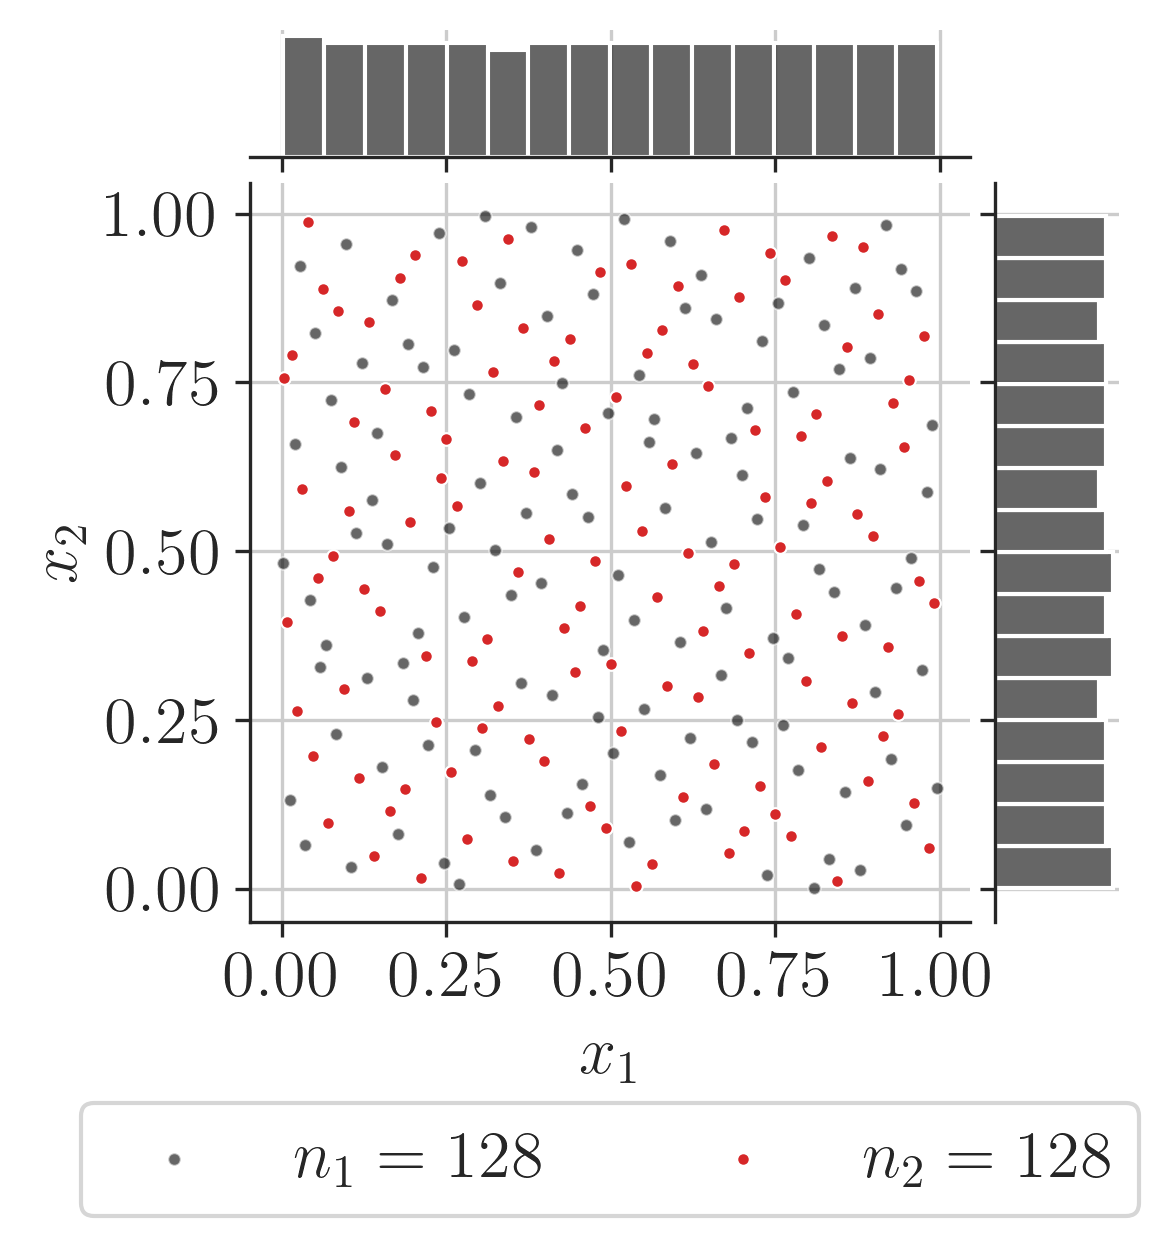
\includegraphics[width=\textwidth]{../numerical_experiments/chapter1/figures/quasi_MonteCarlo_Halton_256.png}
        \caption{Halton sequence.}
    \end{subfigure}
    \hfill
    \begin{subfigure}[b]{0.32\textwidth}
        \centering
        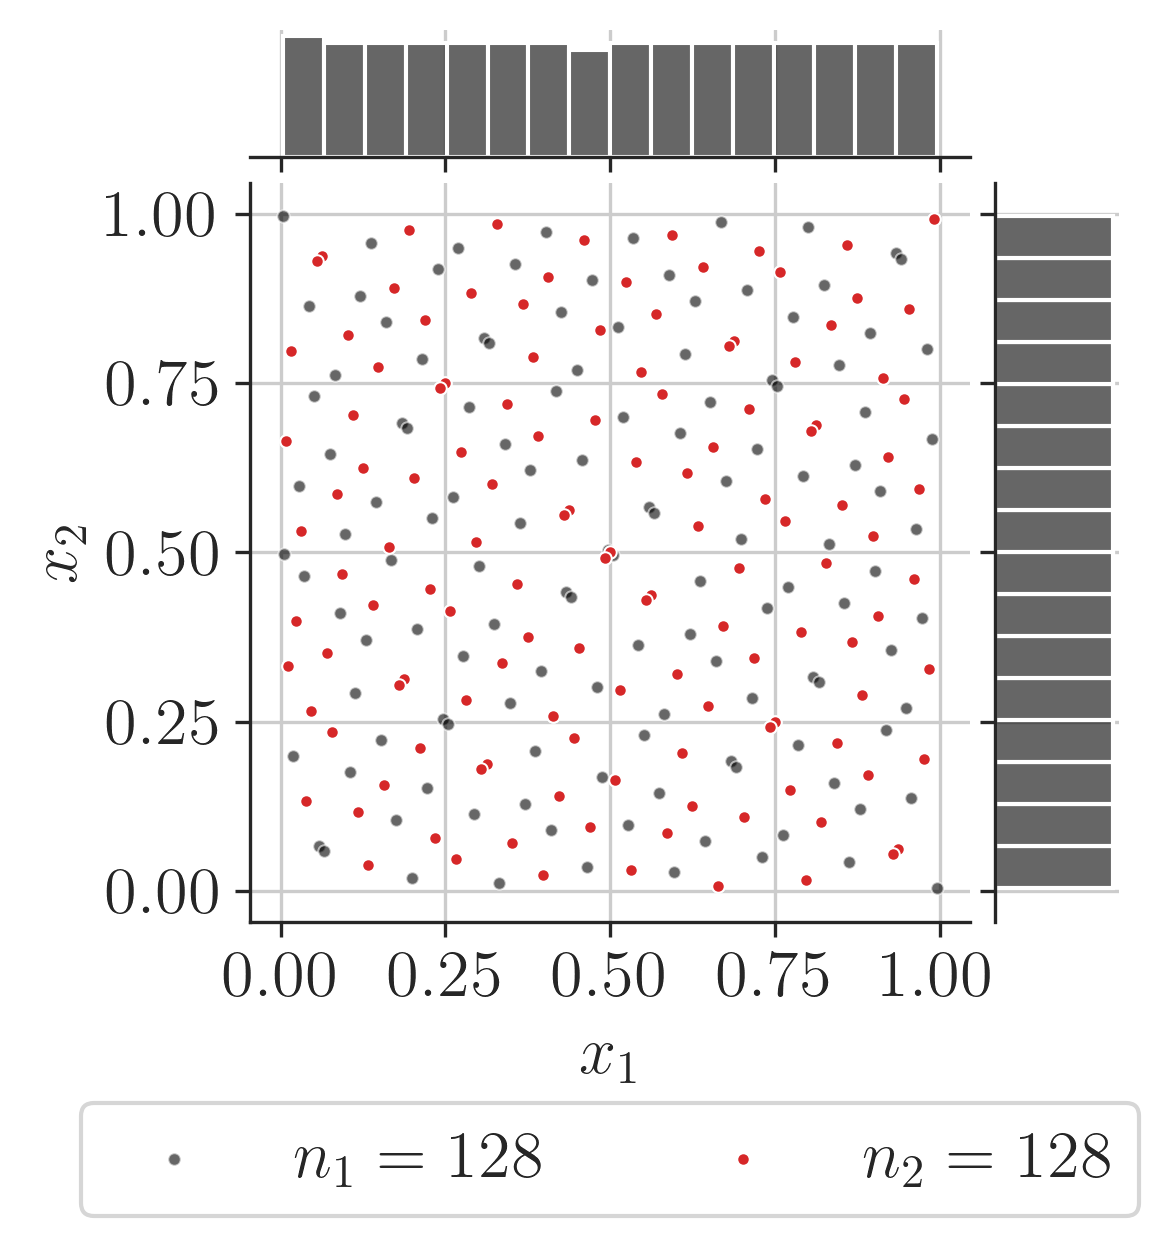
\includegraphics[width=\textwidth]{../numerical_experiments/chapter1/figures/quasi_MonteCarlo_256.png}
        \caption{Sobol' sequence.}
    \end{subfigure}
       \caption{Nested Monte Carlo and quasi-Monte Carlo designs ($n=2^8=256$).}
       \label{fig:quasi_monte_carlo_designs}
\end{figure}

Crude Monte Carlo estimators provide guarantees associated with the estimate. 
This complementary information is essential to deliver an end-to-end UQ, which is missed in deterministic QMC methods.  
\textit{Randomized quasi-Monte Carlo} extends the usual QMC methods by introducing some randomness in order to compute confidence intervals while benefiting from a low variance. 
A specific review of the randomized (also called ``scrambled'') QMC is proposed by \citet{lecuyer_2018}. 
Various authors recommend the use of randomized QMC by default instead of QMC as a good practice (e.g., \citealp{owen_2013}). 
Recent works aim at exploring the use of these methods to estimate different quantities of interest, such as an expected value similar to $I_{\P_{\bX}}(g)$ \citep{gobet_2022} or a quantile \citep{tuffin_2019}. 

Ultimately, QMC methods generate powerful integration schemes. 
The Koksma-Hlawka inequality associates an upper bound and a convergence rate to most integrals. 
A randomization overlay removes the deterministic property of these designs, allowing to compute confidence intervals. 
In the following, sampling techniques are presented from the numerical \textit{design of experiments} point of view. 
Even if the goal might look different from numerical integration, these two topics share many methods and concepts. 


%%%%%%%%%%%%%%%%%%%%%%%%%%%%%%%%%%%%%%%%%%%%%%%%%%%%%%%%%%%%%%
\begin{otexample}[\href{https://github.com/efekhari27/thesis/blob/main/numerical_experiments/chapter1/integration.ipynb}{Numerical integration}]
    A minimal working example in Python is available in Appendix~\ref{apx:D}. 
    Figures illustrating the present section may be reproduced, using the \ots scripts available on the GitHub repository\footnotemark.  
\end{otexample}
%%%%%%%%%%%%%%%%%%%%%%%%%%%%%%%%%%%%%%%%%%%%%%%%%%%%%%%%%%%%%%
\footnotetext{\url{https://github.com/efekhari27/thesis/blob/main/numerical_experiments/chapter1/integration.ipynb}}

%============================================================%
\subsection{Numerical design of experiments} \label{sec:LHS}
%============================================================%
The numerical design of experiments aims at uniformly exploring the input domain, e.g., to build a learning set for a regression model, or to initialize a multi-start optimization strategy. 
A design of experiment (also simply called ``design'') is called \textit{space-filling} when it uniformly covers a domain. 
Such designs can be used to propagate uncertainties for a very limited sample size. 
Therefore, users of designs of experiments consider various properties: 
\begin{itemize}
    \item A first desirable property is the sequentiality of the method, to eventually add new points when their initial computational budget is extended; 
    \item A second quality is the preservation of the methods' properties in any subdomains (i.e., subprojections of the inputs’ domain). 
    This second property can be useful to reduce the problem's dimension by dropping a few unimportant variables (see the following Section~\ref{sec:gsa} on global sensitivity analysis).
\end{itemize}
Different metrics are commonly used to quantify how space-filling a design of experiments is. 
The previously introduced discrepancies are an example of space-filling metrics. 
Other types of space-filling metrics rely on purely geometrical considerations.  

This subsection will first define a few space-filling metrics. 
Secondly, the \textit{Latin hypercube sampling} (\abv{lhs}) will be introduced as a variance-reduction method that became popular in the UQ community. 
Finally, a general discussion on uncertainty propagation w.r.t. non-uniform measures will be presented.

%------------------------------------------------------------%
\subsubsection{Space-filling metrics and properties}
%------------------------------------------------------------%
Space-filling criteria are key to evaluating designs and are often used to optimize their performances. 
In the previous section, the star discrepancy was introduced as a distance of a finite design to uniformity. 
While, the $L_\infty$ star discrepancy is hard to estimate in practice, \citet{warnock_1972} elaborated an explicit expression specific to the $L_2$ star discrepancy: 
\begin{equation}
    D^*_2(\bX_n) = \left(\frac19 - \frac2n \sum_{i=1}^{n} \prod_{l=1}^{d} \frac{(1-x_l^{(i)})}{2} + \frac{1}{n^2}\sum_{i,j=1}^{n} \prod_{l=1}^{d} \left[1 - \max(x_l^{(i)}, x_l^{(j)})\right]\right)^{1/2}.
\end{equation}
One can notice that this expression is similar to the Cram\'{e}r-von Mises test statistic. 
Even if this expression is tractable, \citet{fang_liu_2018} detailed its limits: 
the star $L_2$ discrepancy generates designs that are not robust to projections in sub-spaces; 
it is not invariant by rotation and reflection; 
and finally, by construction, $L_p$ discrepancies give a disproportionate role to the point $\mathbf{0}$ by anchoring the box $[\mathbf{0}, \bx)$.

Two improved criteria were proposed by \citet{hickernell_1998} with the \textit{centered $L_2$ discrepancy} and the \textit{wrap-around $L_2$ discrepancy}. 
Those are widely used in practice since they solve the previous limits while satisfying the Koksma-Hlawka inequality with a modification of the Hardy-Klause variation. 
Let us introduce the explicit formula of the centered $L_2$ discrepancy given by \citet{hickernell_1998}:
\begin{multline} CD^*_2(\bX_n)  = \left(\frac{13}{12}\right)^{d} - \frac{2}{n} \sum_{i=1}^{n} \prod_{l=1}^{d} \left( 1 + \frac{1}{2} |x_l^{(i)} - 0.5| - \frac{1}{2} |x_l^{(i)} - 0.5|^2 \right)\\
    + \frac{1}{n^2} \sum_{i,j=1}^{n} \prod_{l=1}^{d} \left( 1 + \frac{1}{2} |x_l^{(i)} - 0.5| + \frac{1}{2} |x_l^{(j)} - 0.5| - \frac{1}{2} |x_l^{(i)} - x_l^{(j)}| \right).
\end{multline}

As an alternative to discrepancies, many geometrical criteria exist to assess a space-filling design. 
The most common way to do so is to maximize the minimal distance among the pairs of Euclidian distances between the points of a design.  
The criterion to maximize is then simply called the \textit{minimal distance} of a design (denoted by $\phi_{min}$). 
For numerical reasons, the $\phi_p$ criterion is often used instead of the minimal distance. 
The following $\phi_p$ criterion converges towards the minimum distance $\phi_{min}$ as $p\geq1$ tends to infinity:
\begin{equation} 
    \phi_{\min}(\bX_n) = \min_{i \neq j} ||\bx^{(i)} - \bx^{(j)}||_2\, , \qquad
    \phi_p(\bX_n) = \sum_{i=1}^{j} \sum_{j=1}^{n} \left( |x^{(i)} - x^{(j)}|^{-p} \right)^{\frac{1}{p}}\, , \quad i \ne j.
\end{equation}
Further space-filling criteria are reviewed in \citet{abtini_2018} and in \citet[Appendix A]{daveiga_iooss_2021}. 
%Further relationships between some mathematical objects related to space-filling are developed in \citet{pronzato_2012}. 
%These space-filling metrics are widely used to optimize different sampling techniques.


%------------------------------------------------------------%
\subsubsection{Latin hypercube sampling}
%------------------------------------------------------------%
Latin hypercube sampling (LHS) is a method initially introduced in the 1970s as a numerical integration method \citep{mckay_beckman_1979}. 
In a bounded domain, this technique corresponds to a stratified sampling which aims to force the distribution of each sub-projection to be as uniform as possible. 
To do so, for an $n$-sized design, each marginal domain is divided into $n$ identical segments. 
This creates a regular grid of $n^{d}$ squared cells over the domain. 
Then, a latin hypercube design (LHD) does not allow more than one point within a cell. 
That way, new LHDs can be built as a permutation of the marginals of an existing LHD. 
Inside each selected cell from the grid, the point can either be placed at the center of the cell or randomly in the cell.

Various consecutive contributions have explicited the variance, then a central limit theorem to LHS (e.g., \citealp{owen_1992_tcl_lhs}). 
Under monotony hypothesis, the LHS variance can be expressed, when $n\rightarrow\infty$, as:
\begin{equation}
    \var\left(\overline{y}_n^{\textrm{LHS}}\right) = \frac{1}{n} \var\left(g(\bX)\right) - \frac{C}{n} + o\left( \frac1n \right), 
\end{equation}
where $C$ is a positive constant, showing that the LHS usually asymptotically reduces the variance for numerical integration (a proof is proposed in \citealp{stein_1987_lhs}), and $\overline{y}_n^{\textrm{LHS}}$ is the arithmetic mean over the LHS. 
However, because of its stratified structure, LHS can generate poor designs from a space-filling point of view (see e.g., the illustration in \fig{fig:poor_LHS}). 
%Note that LHS was also studied for estimating tail statistics such as quantiles \citep{cannamela_2008_LHS_quantile}.  
The following paragraph presents various methods to optimize LHDs.


%------------------------------------------------------------%
\subsubsection{Optimized Latin hypercube sampling}
%------------------------------------------------------------%
To improve the space-filling property of a LHD, it is common to add an optimization step. 
The goal of this optimization is to improve a space-filling criterion by generating a LHD from permutations of an initial LHD. 
\citet{damblin_couplet_2013} reviewed LHS optimization using different discrepancy criteria and subprojection properties. 
This optimization can be performed by different algorithms, such as the stochastic evolutionary algorithm or simulated annealing. 
The results from this work show that an LHD optimized by the $L_2$ centered or wrap-around discrepancies offers strong robustness to two-dimensional projections. 
It also shows that these designs keep this property for dimensions larger than 10, while scrambled Sobol' sequences may lose it. 
\fig{fig:LHS_designs} illustrates two LHD, optimized by the $L_2$ centered discrepancy and the geometrical $\phi_p$. 
The space-filling difference is not obvious in two-dimensional problems, and they both spread uniformly.    

More recent work developed different ways to optimize LHDs. 
Among them, let us mention the ``maximum projection designs'' (for MaxPro) from \citet{joseph_gul_2015} which rely on the optimization of a geometrical criterion and deliver interesting performances. 
In the same vein, the uniform projection designs from \citet{sun_2019} also optimize LHS, but based on a criterion averaging discrepancies between each pair of marginals.

\begin{figure}[ht]
    \centering
    \begin{subfigure}[b]{0.32\textwidth}
        \centering
        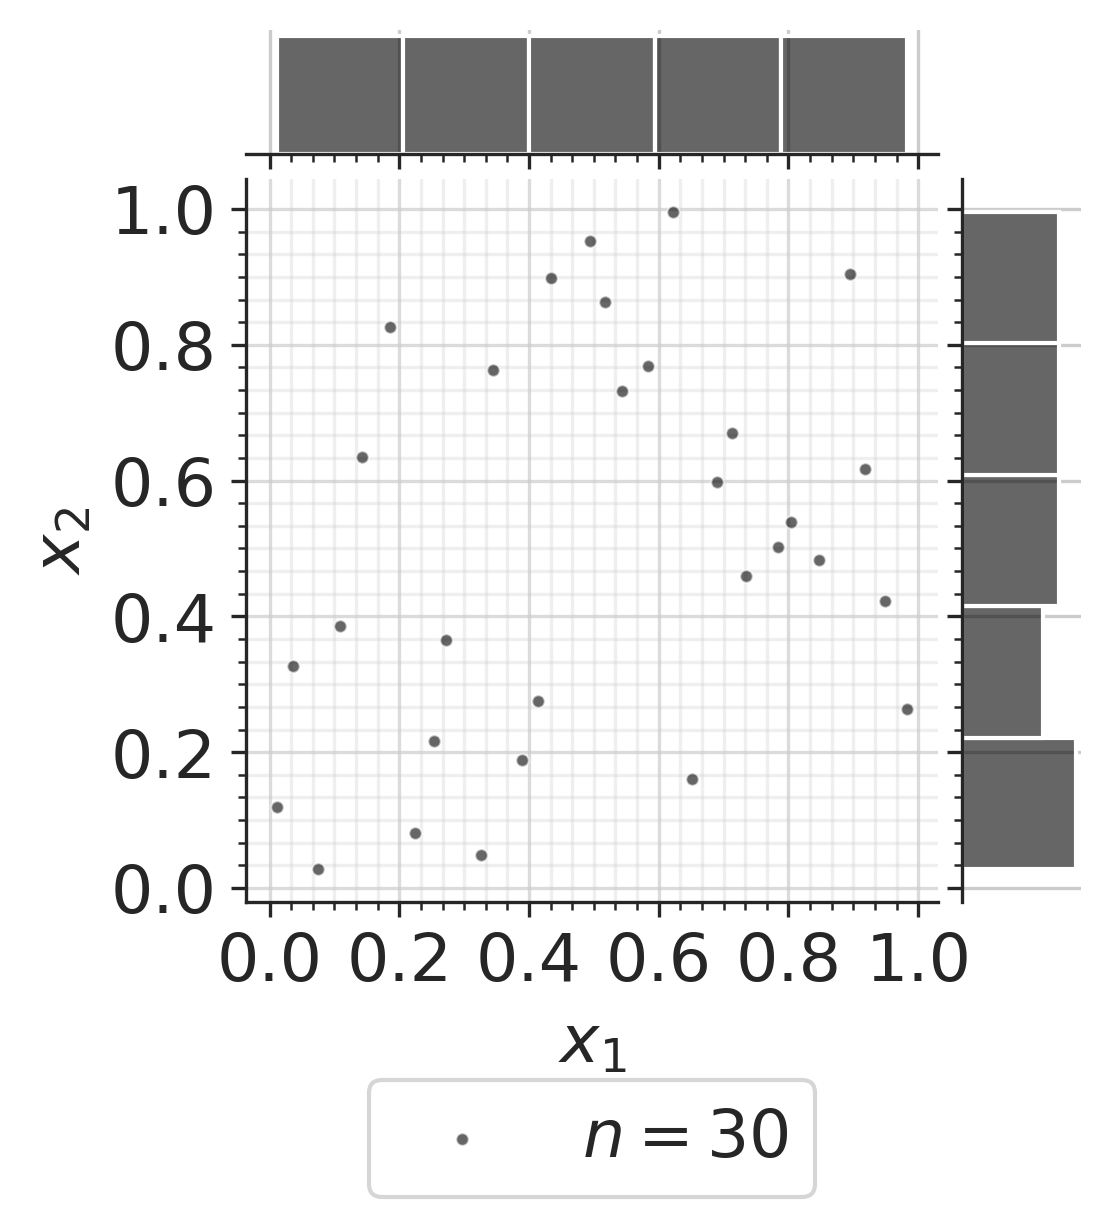
\includegraphics[width=\textwidth]{../numerical_experiments/chapter1/figures/poor_LHS.png}
        \caption{Poorly space-filling LHS.}
        \label{fig:poor_LHS}
    \end{subfigure}
    \hfill
    \begin{subfigure}[b]{0.32\textwidth}
        \centering
        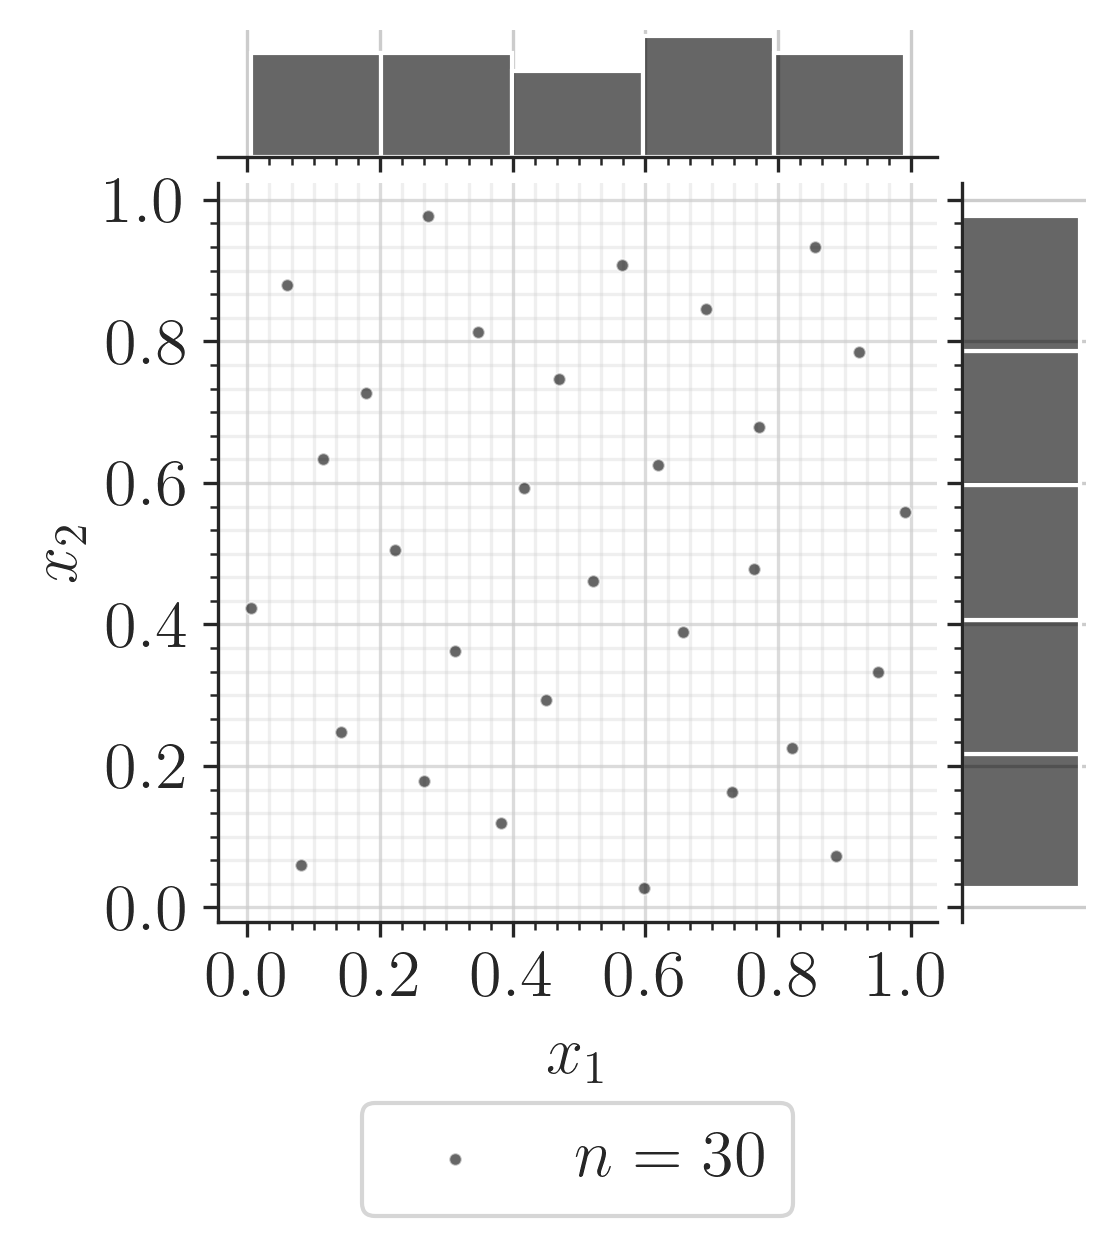
\includegraphics[width=\textwidth]{../numerical_experiments/chapter1/figures/optimized_C2_LHS.png}
        \caption{$L_2$ centered optimized LHS.}
    \end{subfigure}
    \hfill
    \begin{subfigure}[b]{0.32\textwidth}
        \centering
        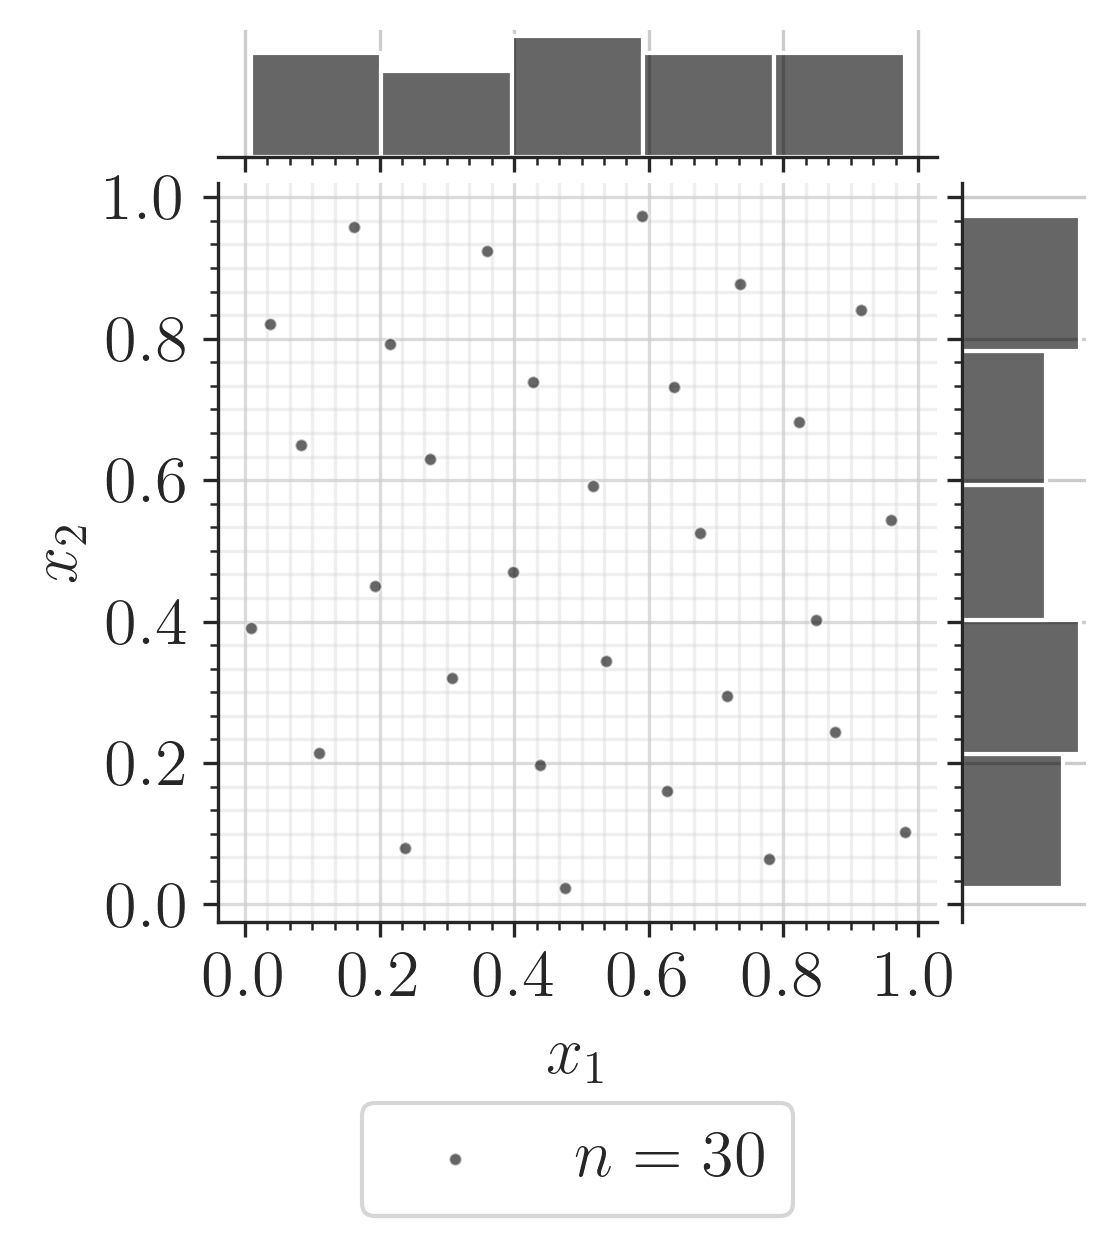
\includegraphics[width=\textwidth]{../numerical_experiments/chapter1/figures/optimized_phip_LHS.png}
        \caption{$\phi_p$ optimized LHS.}
    \end{subfigure}
       \caption{Latin hypercube designs with poor and optimized space-filling properties ($n=30$).}
       \label{fig:LHS_designs}
\end{figure}


%%%%%%%%%%%%%%%%%%%%%%%%%%%%%%%%%%%%%%%%%%%%%%%%%%%%%%%%%%%%%%
\begin{otexample}[\href{https://github.com/efekhari27/thesis/blob/main/numerical_experiments/chapter1/designofexperiments.ipynb}{Design of experiments}]
    A minimal working example in Python is available in Appendix~\ref{apx:D} to build an LHS and 
    an LHS optimized w.r.t. to a space-filling metric (here the L2-centered discrepancy) using the simulated annealing algorithm. 
    Figures illustrating the present section may be reproduced, using the \ots scripts available on the GitHub repository\footnotemark.  
\end{otexample}
%%%%%%%%%%%%%%%%%%%%%%%%%%%%%%%%%%%%%%%%%%%%%%%%%%%%%%%%%%%%%%
\footnotetext{\url{https://github.com/efekhari27/thesis/blob/main/numerical_experiments/chapter1/designofexperiments.ipynb}}

%============================================================%
\subsection{Summary and discussion}
%============================================================%
A wide panel of sampling techniques exists for numerical integration or design of experiments purposes. 
In both cases, the studied domain is bounded and the targeted measure is uniform. 
However, uncertainty propagation is often performed on complex input distributions, with possibly unbounded domains. 
In UQ, this step might be referred to as central tendency estimation (i.e., estimating the output's mean and variance). 
Central tendency estimation can be viewed as a numerical integration w.r.t. an input distribution, sometimes called by authors \textit{probabilistic integration} \citep{briol_oates_2019}, as part of what is called \textit{probabilistic numerics} \citep{oates_sullivan_2019}.  

%To generate i.i.d. samples following any distribution (i.e., non-uniform), one may use \textit{inverse transform} sampling. 
%After generating samples in the unit hypercube, the inverse CDF function (i.e., quantile function) is applied to the marginals. 
%Finally, possible dependence effects may be added using the Sklar theorem \eq{thm:sklar}.

One may wonder if the properties from the uniform design are conserved after this nonlinear transformation. 
\citet{hickernell_2020} explores this question from a discrepancy point of view. 
The authors find correspondences between discrepancies w.r.t. uniformity and discrepancies w.r.t. the target distribution. 
%However, this result shows practical limits, sometimes making the interpretation of the last discrepancy easier. 
This question will be further discussed in Chapter~\ref{chpt:4} and in \citet{fekhari_DCE_2023}, using a more general dissimilarity measure.

%Let us also remark that, depending on the distribution, defining the inverse CDF is not always possible. 
%For example, samples following truncated distributions or mixture distributions might sometimes be generated with a different technique. 
%The \textit{acceptance-rejection} method offers a versatile generation only based on the PDF $f_{\bx}$. 
%Assuming that a well-known proposal PDF $f^*_{\bx}$ exists such that $f_{\bx} \leq c \times f^*_{\bx}, c \in [1, +\infty]$. 
%One may generate a sample according to $c \times f^*_{\bx}$ and only retain from this sample the points under the PDF $f_{\bx}$. 
%%\elias{add illustration with truncated normal and triangular.}
%Note that some sampling methods, such as QMC, are not well suited to acceptance-rejection since their structure gets perturbed. 

In the present section, many methods were presented to propagate input uncertainties against a deterministic function. 
Uncertainty propagation with the three following goals and contexts was introduced: 
\begin{itemize}
    \item building a quadrature rule for numerical integration against a uniform distribution;
    \item creating a space-filling design of experiments to uniformly explore the space, often in a small data context (e.g., to build the learning set of a surrogate model);
    \item generating a design for central tendency estimation, i.e., to perform a numerical integration against a nonuniform density.
\end{itemize} 
%Note that some of these methods can also find use in the context of data compression or quantization.
These three objectives have been explored in different communities, but they actually share similar methods. 
They all have in common the analysis of the central behavior of the output random variable. 
However, some studies require to shift the focus toward specific areas of the output random variables distribution. 
When using uncertainty propagation to perform risk analysis, the events studied are mostly contained in the tails of the output distribution. 
In this case, dedicated uncertainty propagation methods will significantly improve the estimation of the associated statistical quantities.


%============================================================%
%============================================================%
\section{Uncertainty propagation for rare event estimation} \label{sec:reliability}
%============================================================%
%============================================================%

This section aims to present another type of problem often encountered in uncertainty propagation. 
The goal of these problems is to assess the risk or reliability of a critical engineering system. 
Most often, a risk measure associated with a failure mode of the studied system has to be estimated. 

Since most systems studied in risk analysis must be highly reliable, the occurrence of such an event is qualified as rare. 
Only a small amount of input conditions or an unlikely unfavorable combination of inputs leads to the failure of the system. 
Therefore, the equivalent terms \textit{reliability analysis} and \textit{rare event estimation} are used. 
The notion of risk associated with an event is often decomposed as a product of its probability of occurrence and its consequences. 
The failure of a system might be very rare, but its consequences can be severe (e.g., civil engineering structures, nuclear infrastructure, telecommunication networks, electrical grid, railway signaling, etc.).

Different risk measures (i.e., quantities of interest related to the tail of the distributions) can be studied depending on the type of risk analysis. 
Quantiles are a risk measure, widely used for risk analysis. 
The quantile of order $\alpha$, also called $\alpha$-quantile, denoted by $q_\alpha$(Y), of the output random variable $Y$ is defined as:
\begin{equation}
    q_\alpha(Y) = \inf_{y\in\R}{\left\{F_Y(y) \geq \alpha\right\}}, \quad \alpha \in [0, 1].    
\end{equation}
As an alternative, one can define a scalar safety threshold $\yth \in \R$ that should not be exceeded to keep the system safe. 
Then, another risk measure is the probability of crossing this safety threshold, also called \textit{failure probability}, and given by: 
\begin{equation}
    \pf = \P\left(Y \geq \yth\right).
    \label{eq:failure_proba}
\end{equation}
To illustrate this quantity, \fig{fig:1D_reliability} shows the one-dimensional propagation of a normal distribution (represented by the PDF on the left), through a function $\iM(\cdot)$ such that $Y=\iM(X)$.
The probability of crossing a given threshold $\yth$ is represented by the area in red under the output PDF on top.
More information about the use and the interpretation of risk measures including measures from the finance domain such as the \textit{conditional value-at-risk} (also called ``superquantile'') is presented in \citet{rockafellar_2015}. 

\begin{figure}
    \centering
    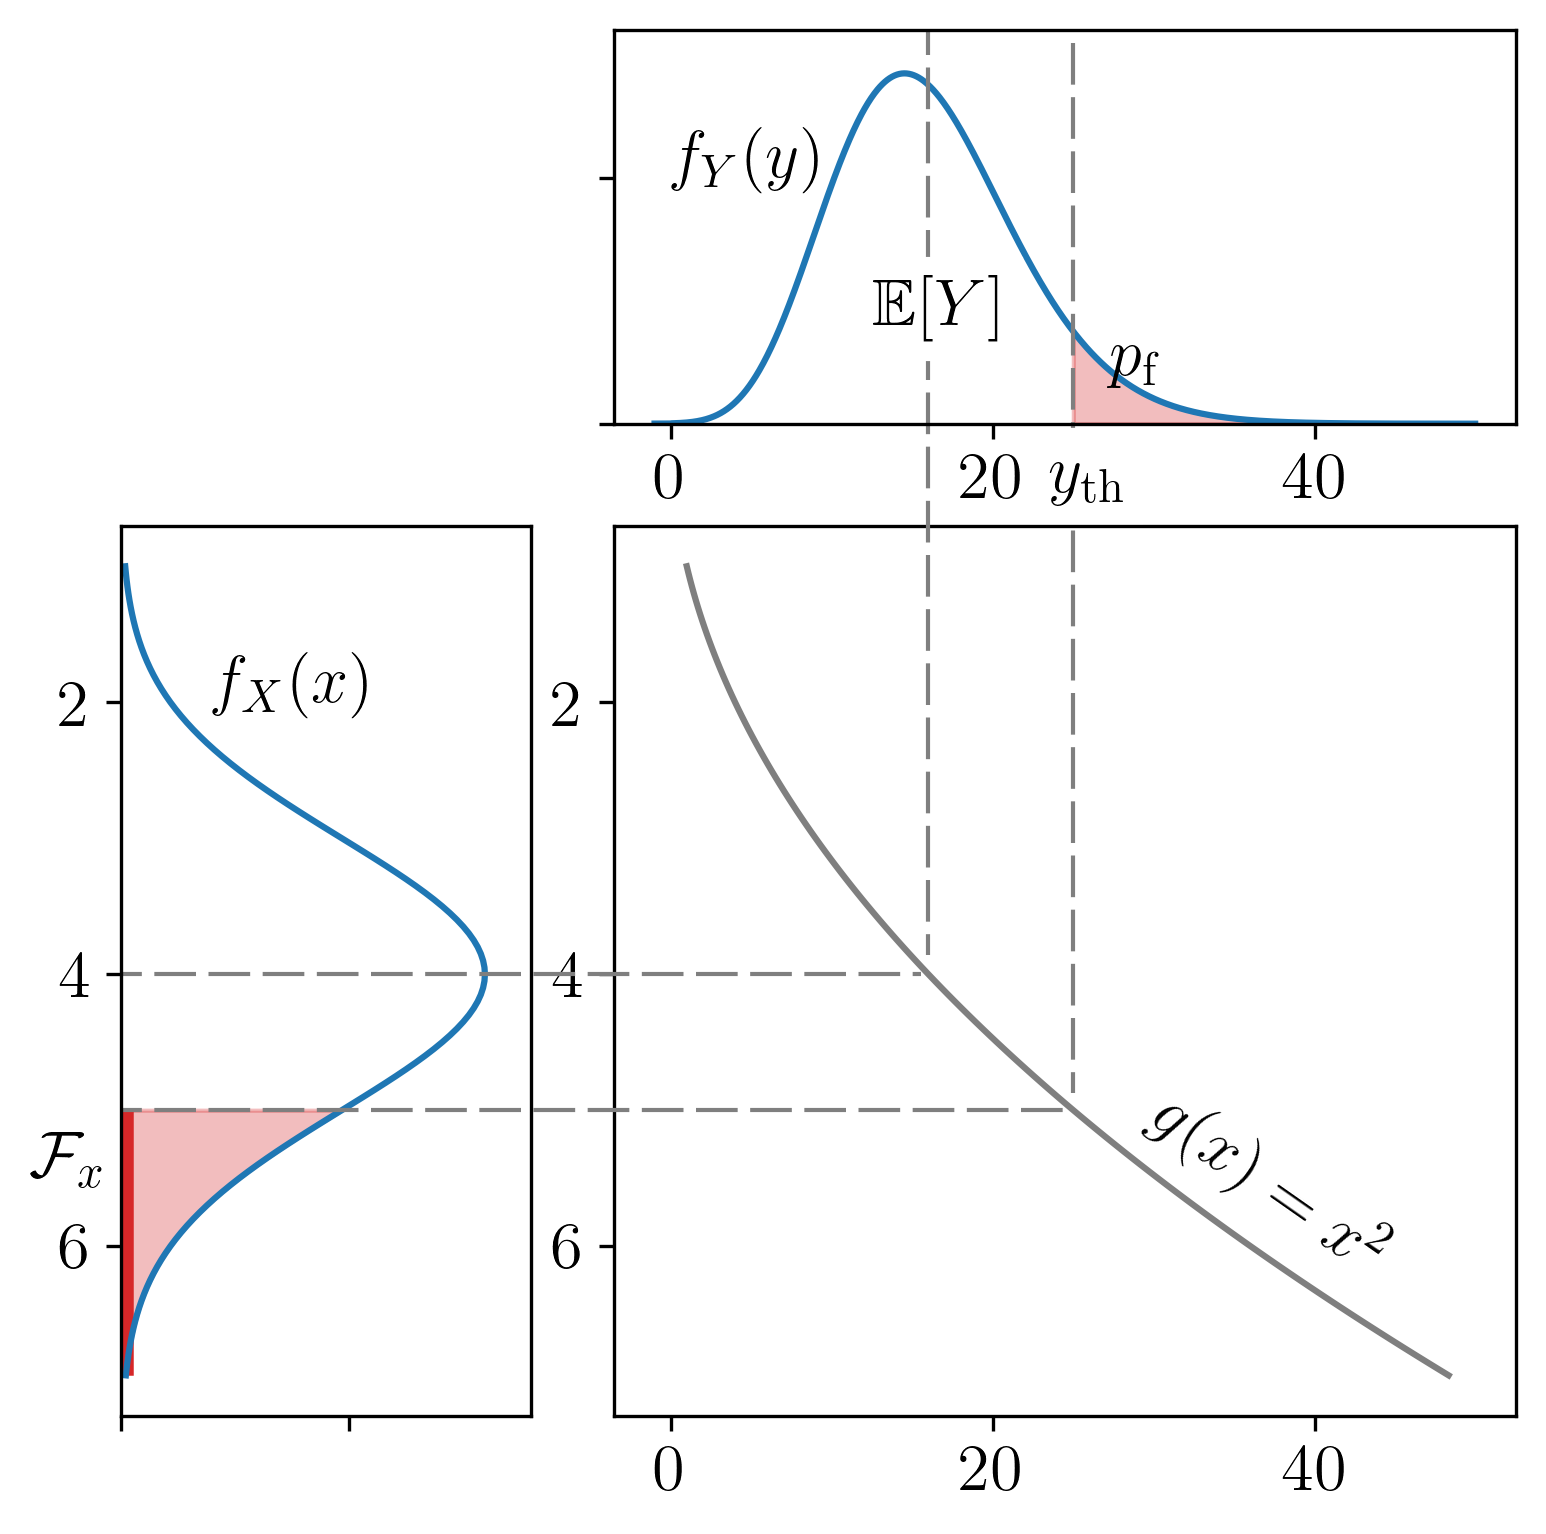
\includegraphics[width=0.5\textwidth]{../numerical_experiments/chapter1/figures/1D_reliability.png}
    \caption{One-dimensional reliability analysis example.}
    \label{fig:1D_reliability}
\end{figure}

In the following section, the formalism for reliability analysis problems will be first presented, 
then the main methods for solving this specific problem will be introduced. 
Note however that the present work will not address the problems of time-dependent reliability analysis tackled in \citet{rackwitz_2001,andrieu_2004_phi2,hawchar_2017}. 

%============================================================%
\subsection{Problem statement}
%============================================================%

Following the UQ methodology, the behavior of the system is modeled by $\iM(\cdot)$. 
Considering the problem of crossing a safety threshold in \eq{eq:failure_proba}, the system's performance is commonly defined as the difference between the model's output and the safety threshold $\yth\in\R$. 
Formally, the \textit{limit-state function} (\abv{lsf}) is a deterministic function $g:\iD_{\bX}\rightarrow\R$ quantifying this performance: 
\begin{equation}
    g(\bx) = \yth - \iM(\bx).
\end{equation}
Depending on the sign of the output realizations of $g(\bx)$, this function splits the input space into two disjoint and complementary domains called  
the \textit{failure domain} $\iF_{\bx}$, and the \textit{safe domain} $\mathcal{S}_\bx$ which are defined as:
\begin{equation}
    \iF_{\bx} = \{\bx \in \iD_\bx \, | \,  g(\bx) \leq 0\}, \qquad 
    \mathcal{S}_\bx = \{\bx \in \iD_\bx \, | \, g(\bx) > 0\}. 
    %\iD_\bx = \iF_{\bx} \cup \mathcal{S}_\bx 
\end{equation}
The border between these two domains is a hypersurface called \textit{limit-state surface}, and defined by $\iF_{\bx}^0 = \{\bx \in \iD_\bx ~|~ g(\bx) = 0\}$. 
Similarly to any UQ study using a numerical model, this problem may require to be resolved using a limited number of calls to a black-box simulator. 
The difficulties in a reliability problem partially come from the properties of the LSF: nonlinear, costly to evaluate or with a multimodal failure domain. 
Additionally, note that the reliability problem can be the composition of multiple reliability problems, often modeled as a system of sequential and parallel problems \citep{lemaire_2009,derkiureghian_2022_book}.

A rare event estimation results from a particular uncertainty propagation through the LSF. 
%Considering the output variable of interest $g(\bX)$, its probability of being negative (i.e., in the failure domain) is a common risk measure. 
%The so-called \textit{failure probability}, denoted by $\pf$, is the quantity of interest for reliability analysis considered in this work. 
\textit{failure probability}, denoted by $\pf$ is formally written:%\footnotemark: 
\begin{equation}
    \begin{split}
        \pf = \P(Y \geq \yth) &= \P(g(\bX) \leq 0) = \int_{\iF_\bx} f_\bX(\bx) \, \dd\bx
        = \int_{\iD_\bx} \1_{\{\iF_\bx\}}(\bx) f_\bX(\bx) \, \dd\bx .
    \end{split}
    \label{eq:pf}
\end{equation}
%\footnotetext{Note that this probabilistic integration is usually written using the PDF $f_\bX(\cdot)$, but it could identically be expressed in terms of probability measure by taking $f_\bX(\bx) \, \dd\bx = \dd \P_{\bX}(\bx), \, \forall \bx \in \iD_\bx$.}
%where the indicator function applied to the failure domain returns $\1_{\left\{\iF_{\bX}\right\}}(x) = 1$ if $x \in \iF_{\bX}$ and $\1_{\left\{\iF_{\bX}\right\}}(x) = 0$ otherwise. 
Rare event estimation implies both contour finding (i.e., characterizing the LSF) and an estimation strategy targeting the failure domain (with the fewest number of simulations). 
Note that failure events can be qualified as rare when their failure probability has an order of magnitude between $10^{-9} \leq \pf \leq 10^{-2}$ (see e.g., \citealp{lemaire_2009}). 

Instead of directly performing a reliability analysis in the physical space (often called ``$\bx$-space''), these problems are usually solved in the \emph{standard normal space} (also called ``$\bu$-space''). 
Working in the standard normal space reduces numerical issues caused by potentially unscaled or asymmetric marginals. 
Moreover, a larger panel of methods can be applied in the standard normal space since the random inputs become independent.   
The bijective mapping between these two spaces is called an ``iso-probabilistic transformation'', 
denoted by $T: \iD_{\bx} \rightarrow \R^d$, with $\bx \mapsto T(\bx) = \bu = \left(u_1, \dots, u_d\right)\TT$. 
When considering any random vector $\bX = \left(X_1, \dots, X_d\right)\TT$ and the independent standard Gaussian vector $\bU = \left(U_1, \dots, U_d\right)\TT$, the following equivalence holds:
\begin{equation}
    \bU = T(\bX) \Leftrightarrow \bX = T^{-1}(\bU).
\end{equation} 

Thus, a reliability problem can be expressed in the standard normal space. 
In the following, the transformed LSF $\check{g}$ defined as: 
\begin{equation}
    \cg : \bigg|
    \begin{array}{rcl}
        \R^d & \longrightarrow & \R\\
        \bu & \longmapsto & \check{g}(\bu) = \left(g \circ T^{-1}\right)(\bu).
    \end{array}
\end{equation}

Since this transformation is a diffeomorphism\footnote{Considering two manifolds $A$ and $B$, a transformation $T: A \rightarrow B$ is called a diffeomorphism if it is a differentiable bijection with a differentiable inverse $T^{-1}: B \rightarrow A$.}, 
one can apply the change of variable $\bx = T(\bu)$ to express the reliability problem from \eq{eq:pf} in the standard normal space: 
\begin{equation}
    \pf = \P(\cg(\bU) \leq 0) 
        = \int_{\iF_\bu} \varphi_d(\bu) \, \dd\bu 
        = \int_{\R^d} \1_{\{\iF_\bu\}}(\bu) \varphi_d(\bu) \, \dd\bu \,,
\end{equation}
with the transformed failure domain denoted by $\iF_\bu = \{\bu \in \R^d \, | \, \cg(\bu) \leq 0\}$, 
and the $d$-dimensional standard Gaussian PDF $\varphi_d(\bu) = \frac{1}{(2\pi)^{d/2}} \exp\left(-\frac{\lVert\bu\rVert^2_2}{2}\right)$. 
The fact that the failure probability is invariant by this transformation allows the analyst to estimate this quantity in both spaces.  

Different types of transformations exist, such as the Rosenblatt or the generalized Nataf transformation introduced by \citet{lebrun_2013_these}. 
In practice, the transformation choice depends on the properties of the input distribution studied. 
For example in \ot, depending on the three following cases, different types of transformations are applied:
\begin{itemize}
    \item for elliptical distributions, a linear Nataf transformation is applied;
    \item for distributions with an elliptical copula, the generalized Nataf transformation is used \citep{lebrun_2009};
    \item otherwise, the Rosenblatt transformation is used \citep{lebrun_2009_dotheydiff}.
\end{itemize} 



%============================================================%
\subsection{Rare event estimation methods}\label{sec:rare_event}
%============================================================%
%\elias{Why are the previous sampling methods not suited for rare events?}
%\elias{Surrogate based methods can help the contour finding step.}

The main risk measure chosen for rare event estimation in this work is the previously introduced failure probability. 
%Therefore, let us recall that the goal is to build an efficient estimation (or approximation) of the following $d$-dimensional integral: 
%\begin{equation}
%    \pf = \int_{\iD_\bx} \1_{\{\iF_\bx\}}(\bx) f_\bX(\bx) \, \dd\bx.
%\end{equation}
In the computer experiments context, the simulation budget is often limited to $n$ runs with $\pf \ll \frac1n$. 
This explains the need for specific methods offering approximations or simulations targeting the unknown failure domain. 
Two types of rare event estimation methods are classically presented: first, using approximation approaches, and second, using sampling techniques. 
This section introduces the commonly used rare event methods, see \cite{MorioBalesdent2015} for a more exhaustive review.


%------------------------------------------------------------%
\subsubsection{First and second-order reliability methods (FORM/SORM)}
%------------------------------------------------------------%

The well-known first and second-order reliability methods (\abv{form} and SORM) both rely on a geometric approximation to estimate a failure probability \citep{lemaire_2009}. 
They extrapolate a local approximation of the LSF built in the vicinity of a \textit{most-probable-failure-point} (\abv{mpfp}), also called \textit{design point}.

Working in the standard normal space, the methods first look for this MPFP, denoted by $P^*$, with coordinates $\bu^*$. 
To find it, one can solve the following quadratic optimization problem: 
\begin{equation}
    \bu^* = \argmax_{\bu \in \R^d} \left(\1_{\{\iF_\bu\}}(\bu) \varphi_d(\bu)\right).
\end{equation}
Using the properties of the standard normal space allows us to rewrite it as: 
\begin{align}
    \bu^* &= \argmax_{\bu \in \R^d} \, \frac{1}{(2\pi)^{d/2}} \exp\left(-\frac{\bu\TT \bu }{2} \right) \qquad \mathrm{s.t.} \quad \bu \in \iF_{\bu}\\
          &= \argmin_{\bu \in \R^d} \, \bu\TT \bu \qquad \mathrm{s.t.} \quad \cg(\bu) \leq 0.
\end{align}
Such a quadratic optimization under nonlinear constraint is classically solved by gradient descent algorithms (e.g., Abdo-Rackwitz algorithm from \citealp{abdo_rack_1991}) but also by gradient-free techniques (e.g., Cobyla algorithm, see \citealp{powell_1994}). 
The design point corresponds to the smallest Euclidian distance between the limit-state surface and the origin of the standard normal space. 
To understand its role in the reliability problem, let us recall that the density of the standard normal presents an exponential decay in its radial and tangential directions. 
Then, $P^*$ is the failure point with the largest probability density (see the illustration in \fig{fig:FORM_SORM_approx}). 

This distance between the origin and $P^*$ is another risk measure, defined as the \textit{Hasofer-Lind reliability index} \citep{lemaire_2009}, $\beta \in \R$ such that:
\begin{equation}
    \beta = \Vert \bu^* \Vert_2 = \balpha \TT \bu^*, \qquad \mathrm{s.t.} \quad
        \balpha = \frac{\nabla_{\bu} \,  \cg(\bu)}{\Vert \nabla_{\bu} \,  \cg(\bu) \Vert_2}.      
    %= \min_{\cg(\bu)=0} \left(sqrt{\bu\TT\bu}\right)
\end{equation}
The vector $\balpha$ is the unit vector pointing at $P^*$ from the origin point. 

FORM aims at approximating the LSF $\cg(\cdot)$ by its first-order Taylor expansion around the MPFP, denoted by $\cg_1(\bu^*)$: 
\begin{equation}
    \begin{split}
        \cg(\bu) &= \cg_1(\bu^*) + o\left(\Vert \bu - \bu^* \Vert_2^2\right)\\
                 &= \cancel{\cg(\bu^*)} + \nabla_{\bu} \,  \cg(\bu^*)\TT \left(\bu -\bu^* \right) + o\left(\Vert \bu - \bu^* \Vert_2^2\right)\\
                 &= \Vert \nabla_{\bu} \, \cg(\bu) \Vert_2 \left(\balpha\TT \bu^* - \balpha\TT \bu \right) + o\left(\Vert \bu - \bu^* \Vert_2^2\right).
    \end{split}    
\end{equation}
 
Using $\cg_1(\cdot)$ as an approximation of the LSF, the failure probability can be approximated as: 
\begin{equation}
    \pf \approx \pf^{\mathrm{FORM}} = \P\left(- \balpha\TT \bu \leq -\beta\right) = \Phi(-\beta)\, ,
\end{equation} 
with $\Phi(\cdot)$ the CDF of the standard Gaussian. 
Depending on the properties of the LFS, this approximation will be more or less accurate. 
Note that for a purely linear LFS, $\pf = \pf^{\mathrm{FORM}}$. 
When the function is nonlinear, adding a quadratic term to the Taylor expansion can help the approximation. 
The approximation method is then called SORM for \textit{second order reliability method}. 
However, this added complexity implies the computation of Hessian matrices, which can be complicated (see Chapter 1 from \citealp{bourinet_2018} for their estimation).


\begin{figure}[ht]
    \centering
    \begin{subfigure}[b]{0.48\textwidth}
        \centering
        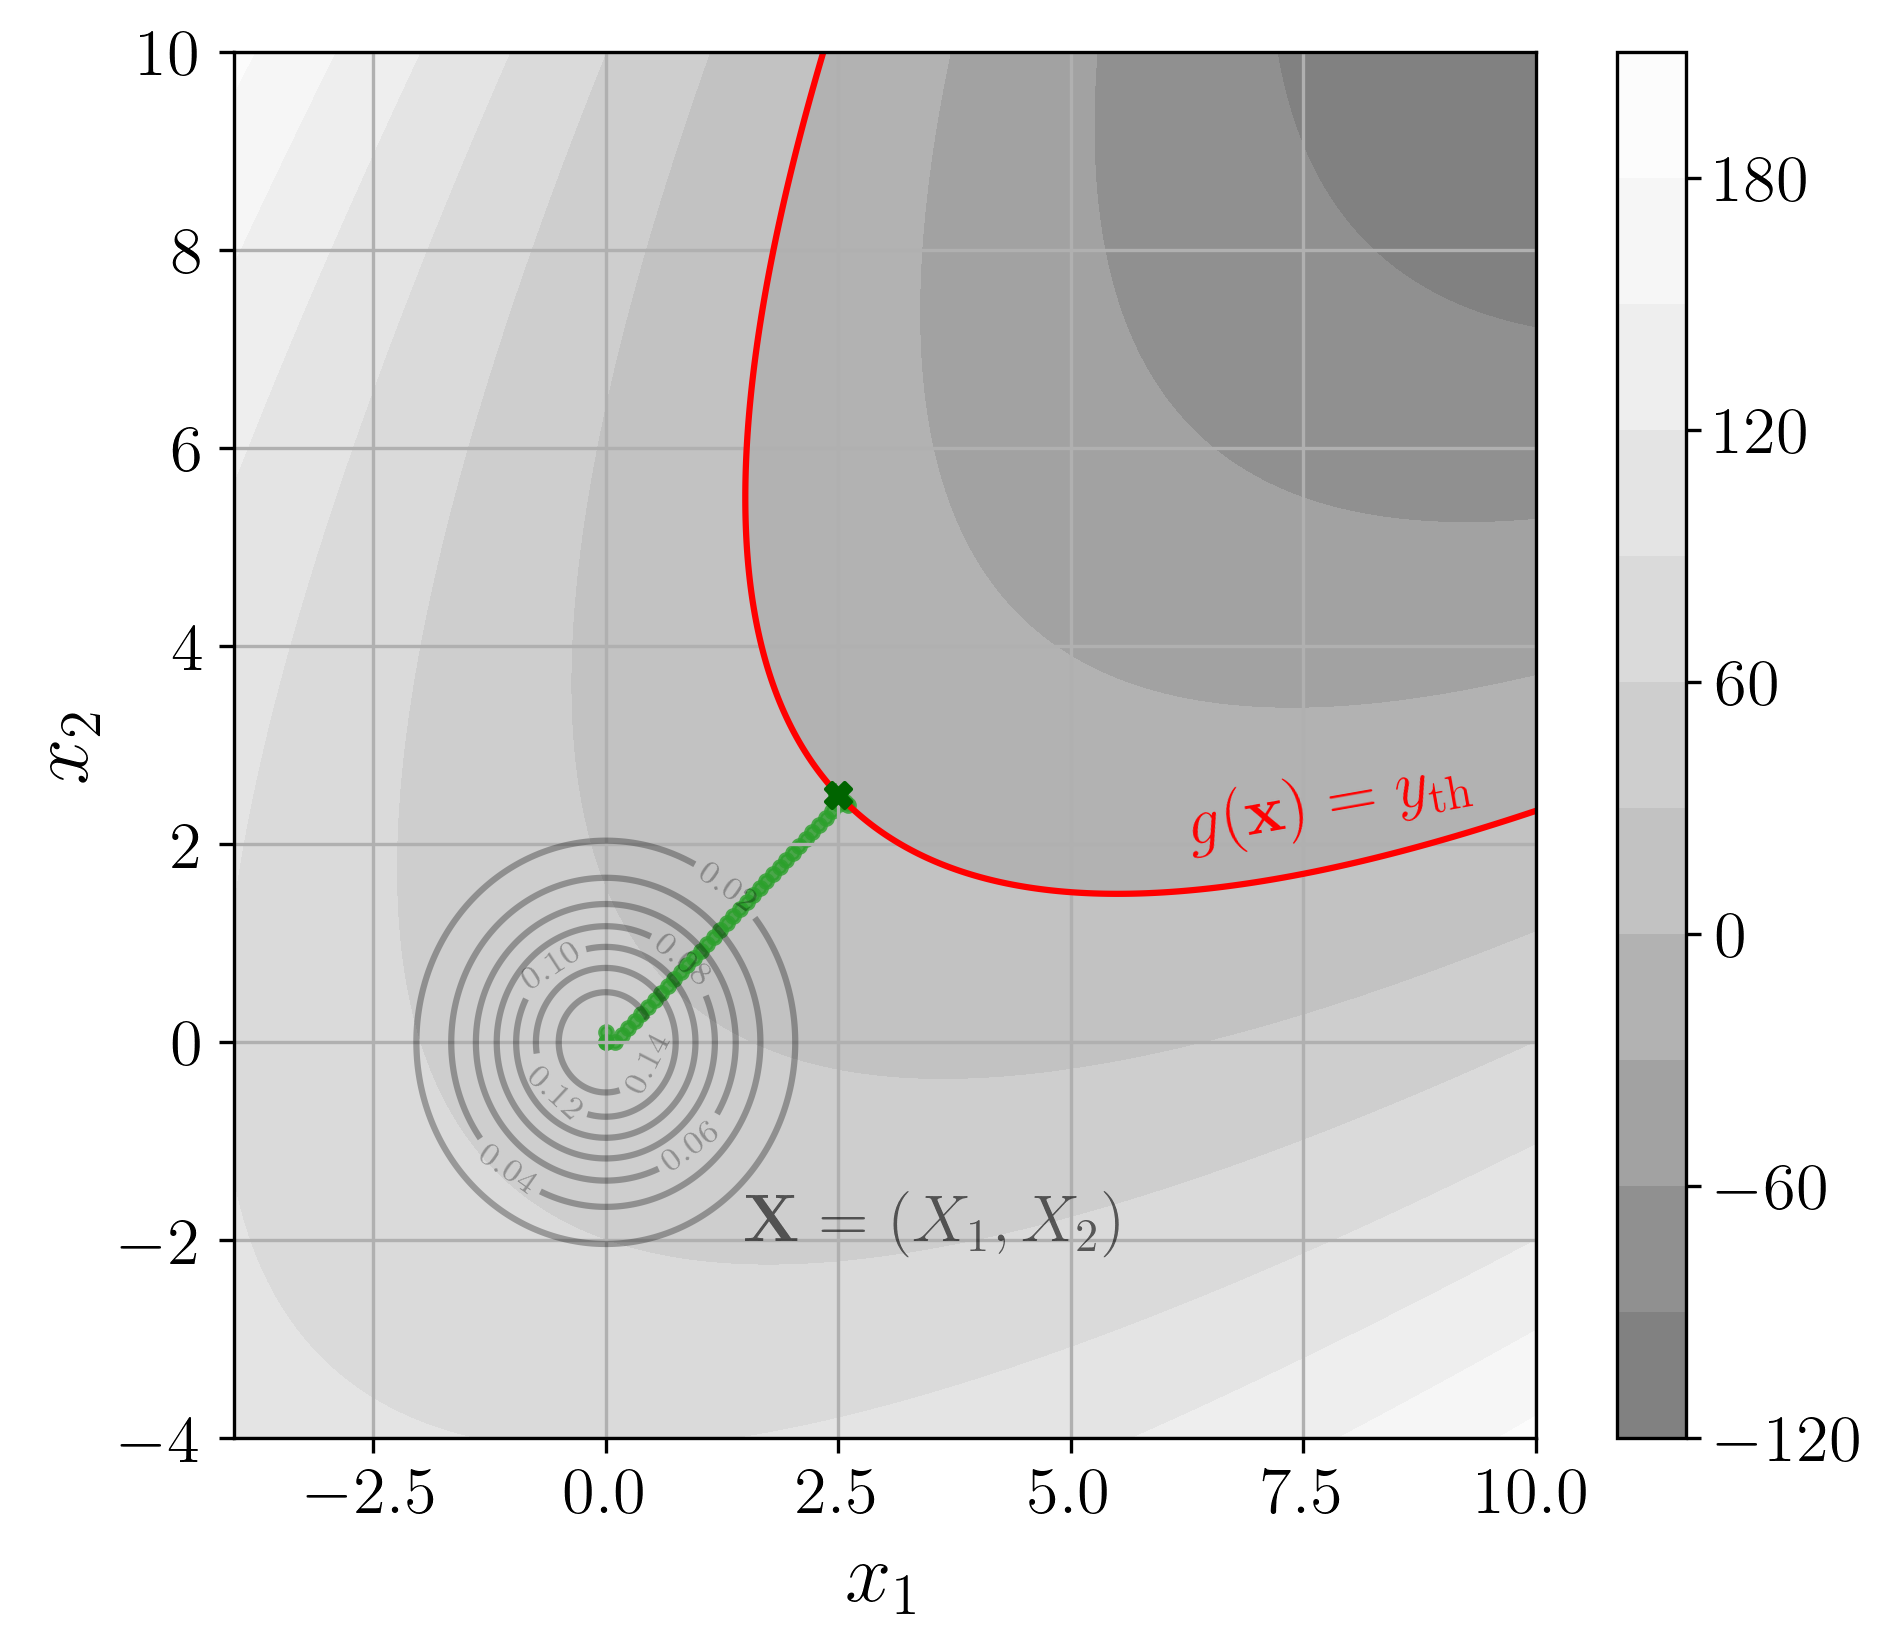
\includegraphics[width=\textwidth]{../numerical_experiments/chapter1/figures/reliability_FORM_illustration.png}
        \caption{FORM approximation.}
    \end{subfigure}
    \quad
    \begin{subfigure}[b]{0.48\textwidth}
        \centering
        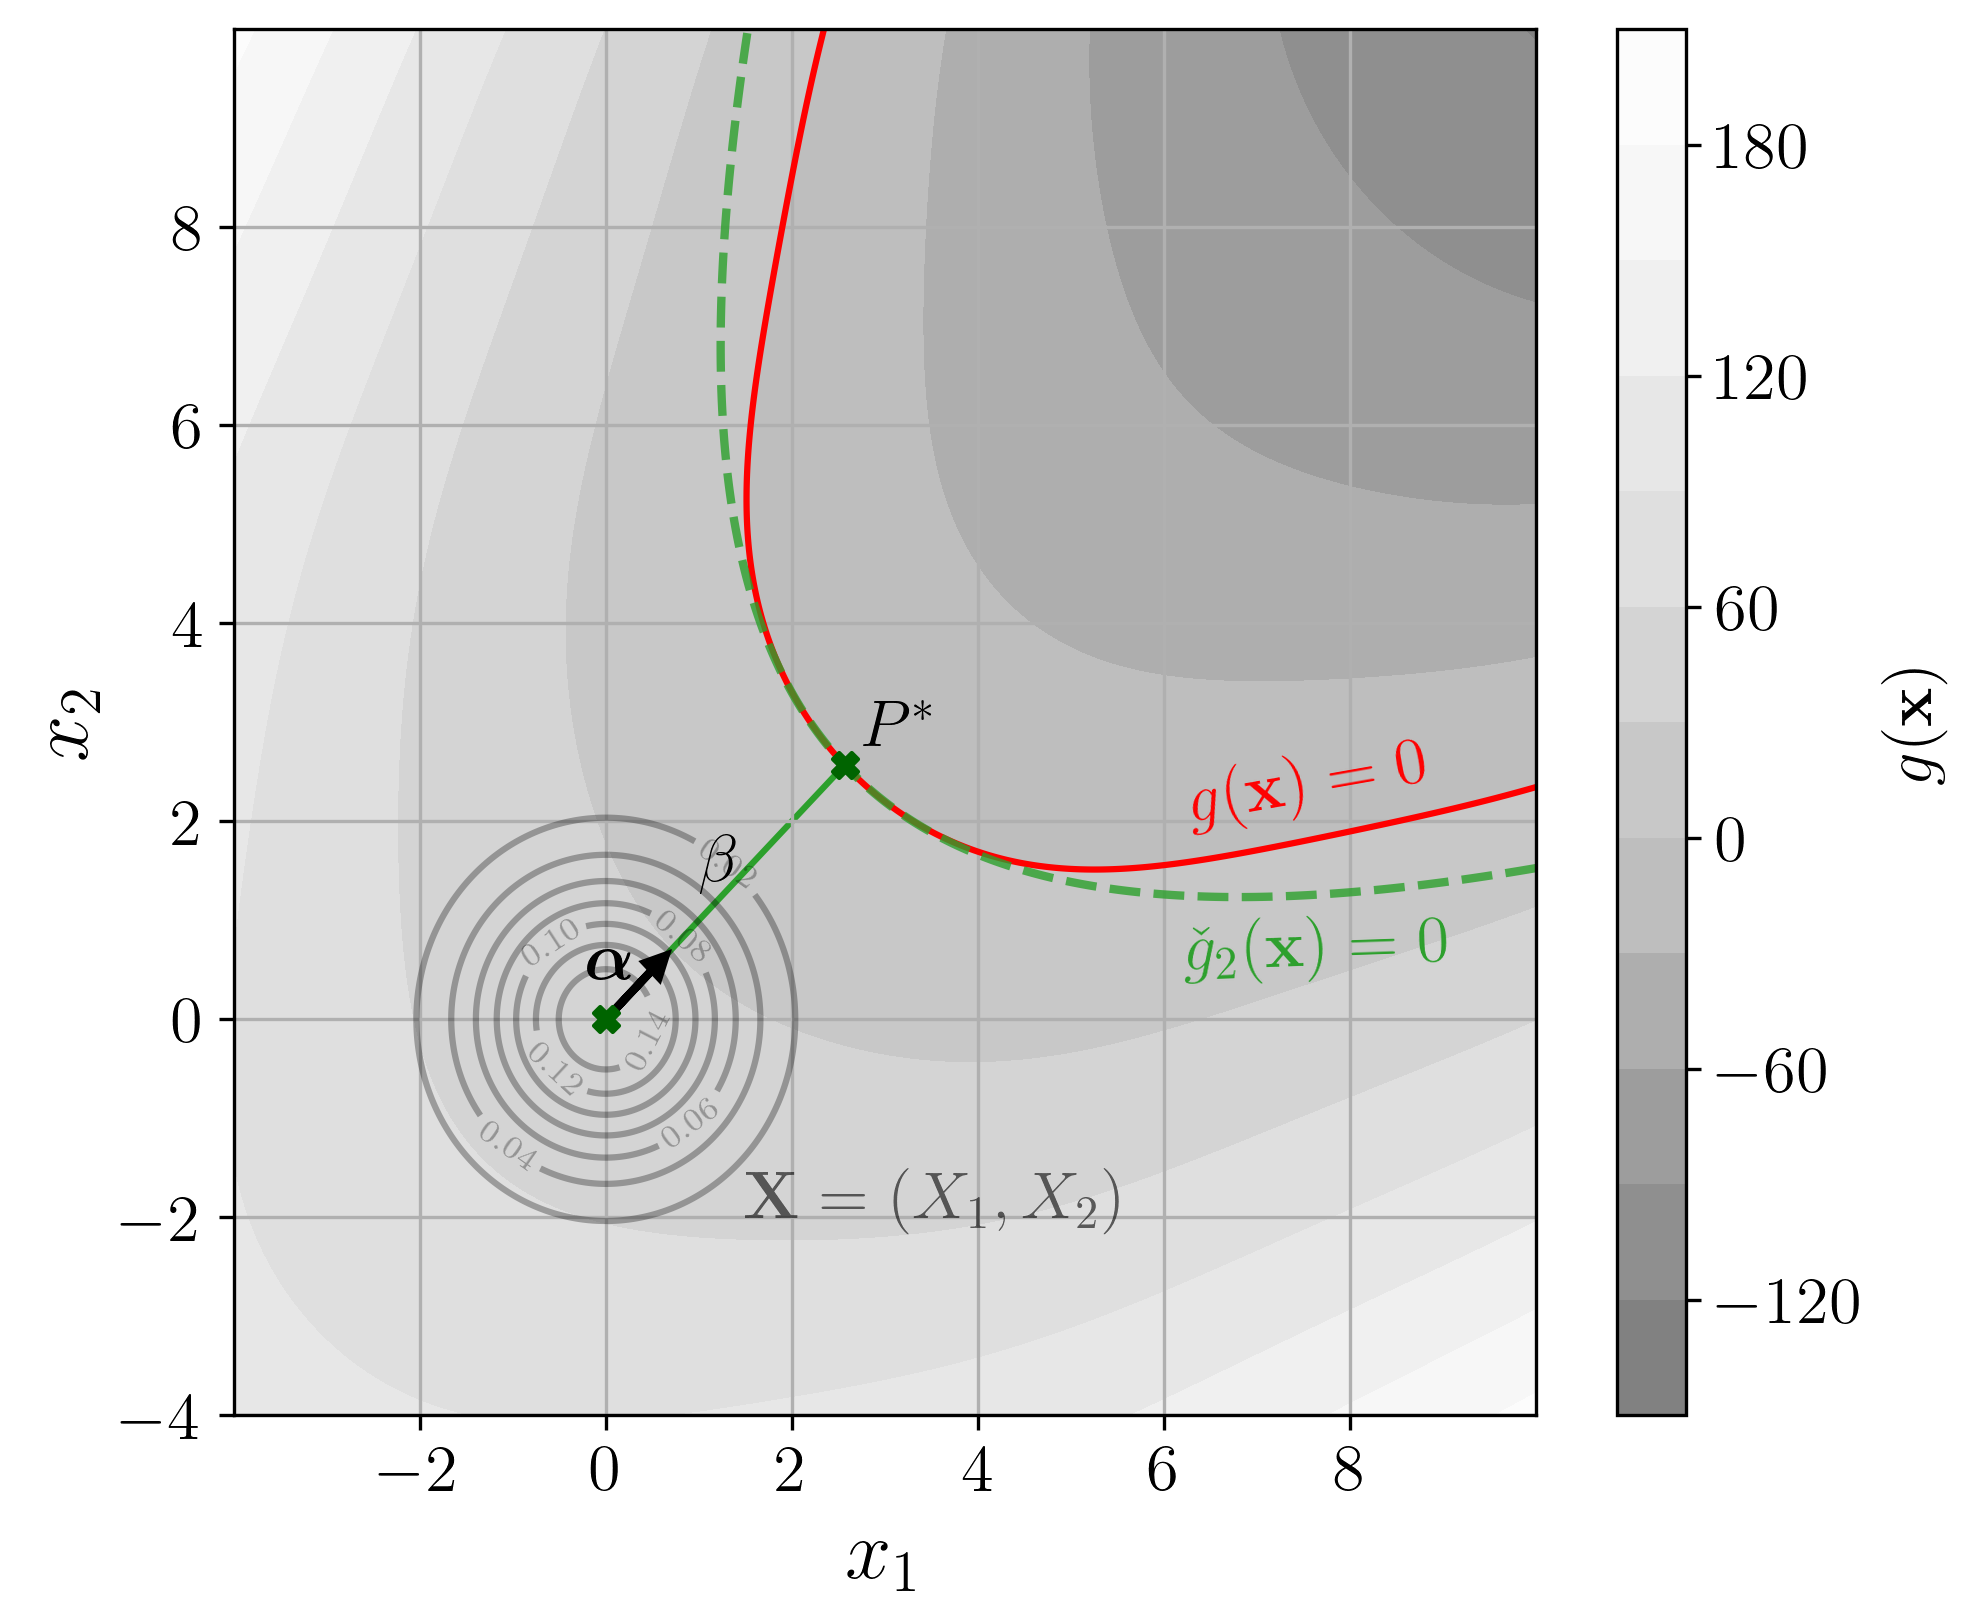
\includegraphics[width=\textwidth]{../numerical_experiments/chapter1/figures/reliability_SORM_illustration.png}
        \caption{SORM approximation.}
    \end{subfigure}
       \caption{FORM and SORM approximation applied to a two-dimensional problem where $g(x_1, x_2)=(x_1 - x_2) ^ 2 - 8 \, (x_1 + x_2 - 5) + \sin(x_1) + \sin(x_2)$.}
       \label{fig:FORM_SORM_approx}
\end{figure}

When the MPFP is not unique, the application of these methods might lead to large errors. 
From a geometrical point of view, having more than one MPFP means that more than one failure zone is at the same Euclidean distance of the origin. 
Applying a FORM or SORM resolution in this particular case leads to the estimation of only one of the failure areas. 
The \textit{muti-FORM} algorithm (see \citet{derkiureghian_1998}) prevents this situation by applying successive FORM. 
Once the first MPFP $P^{*^{(1)}}$ is found, the limit-state surface is modified by removing a nudge to find to following MPFP $P^{*^{(2)}}$, positioned at a similar distance but in a different direction. 

\begin{figure}[ht]
    \centering
    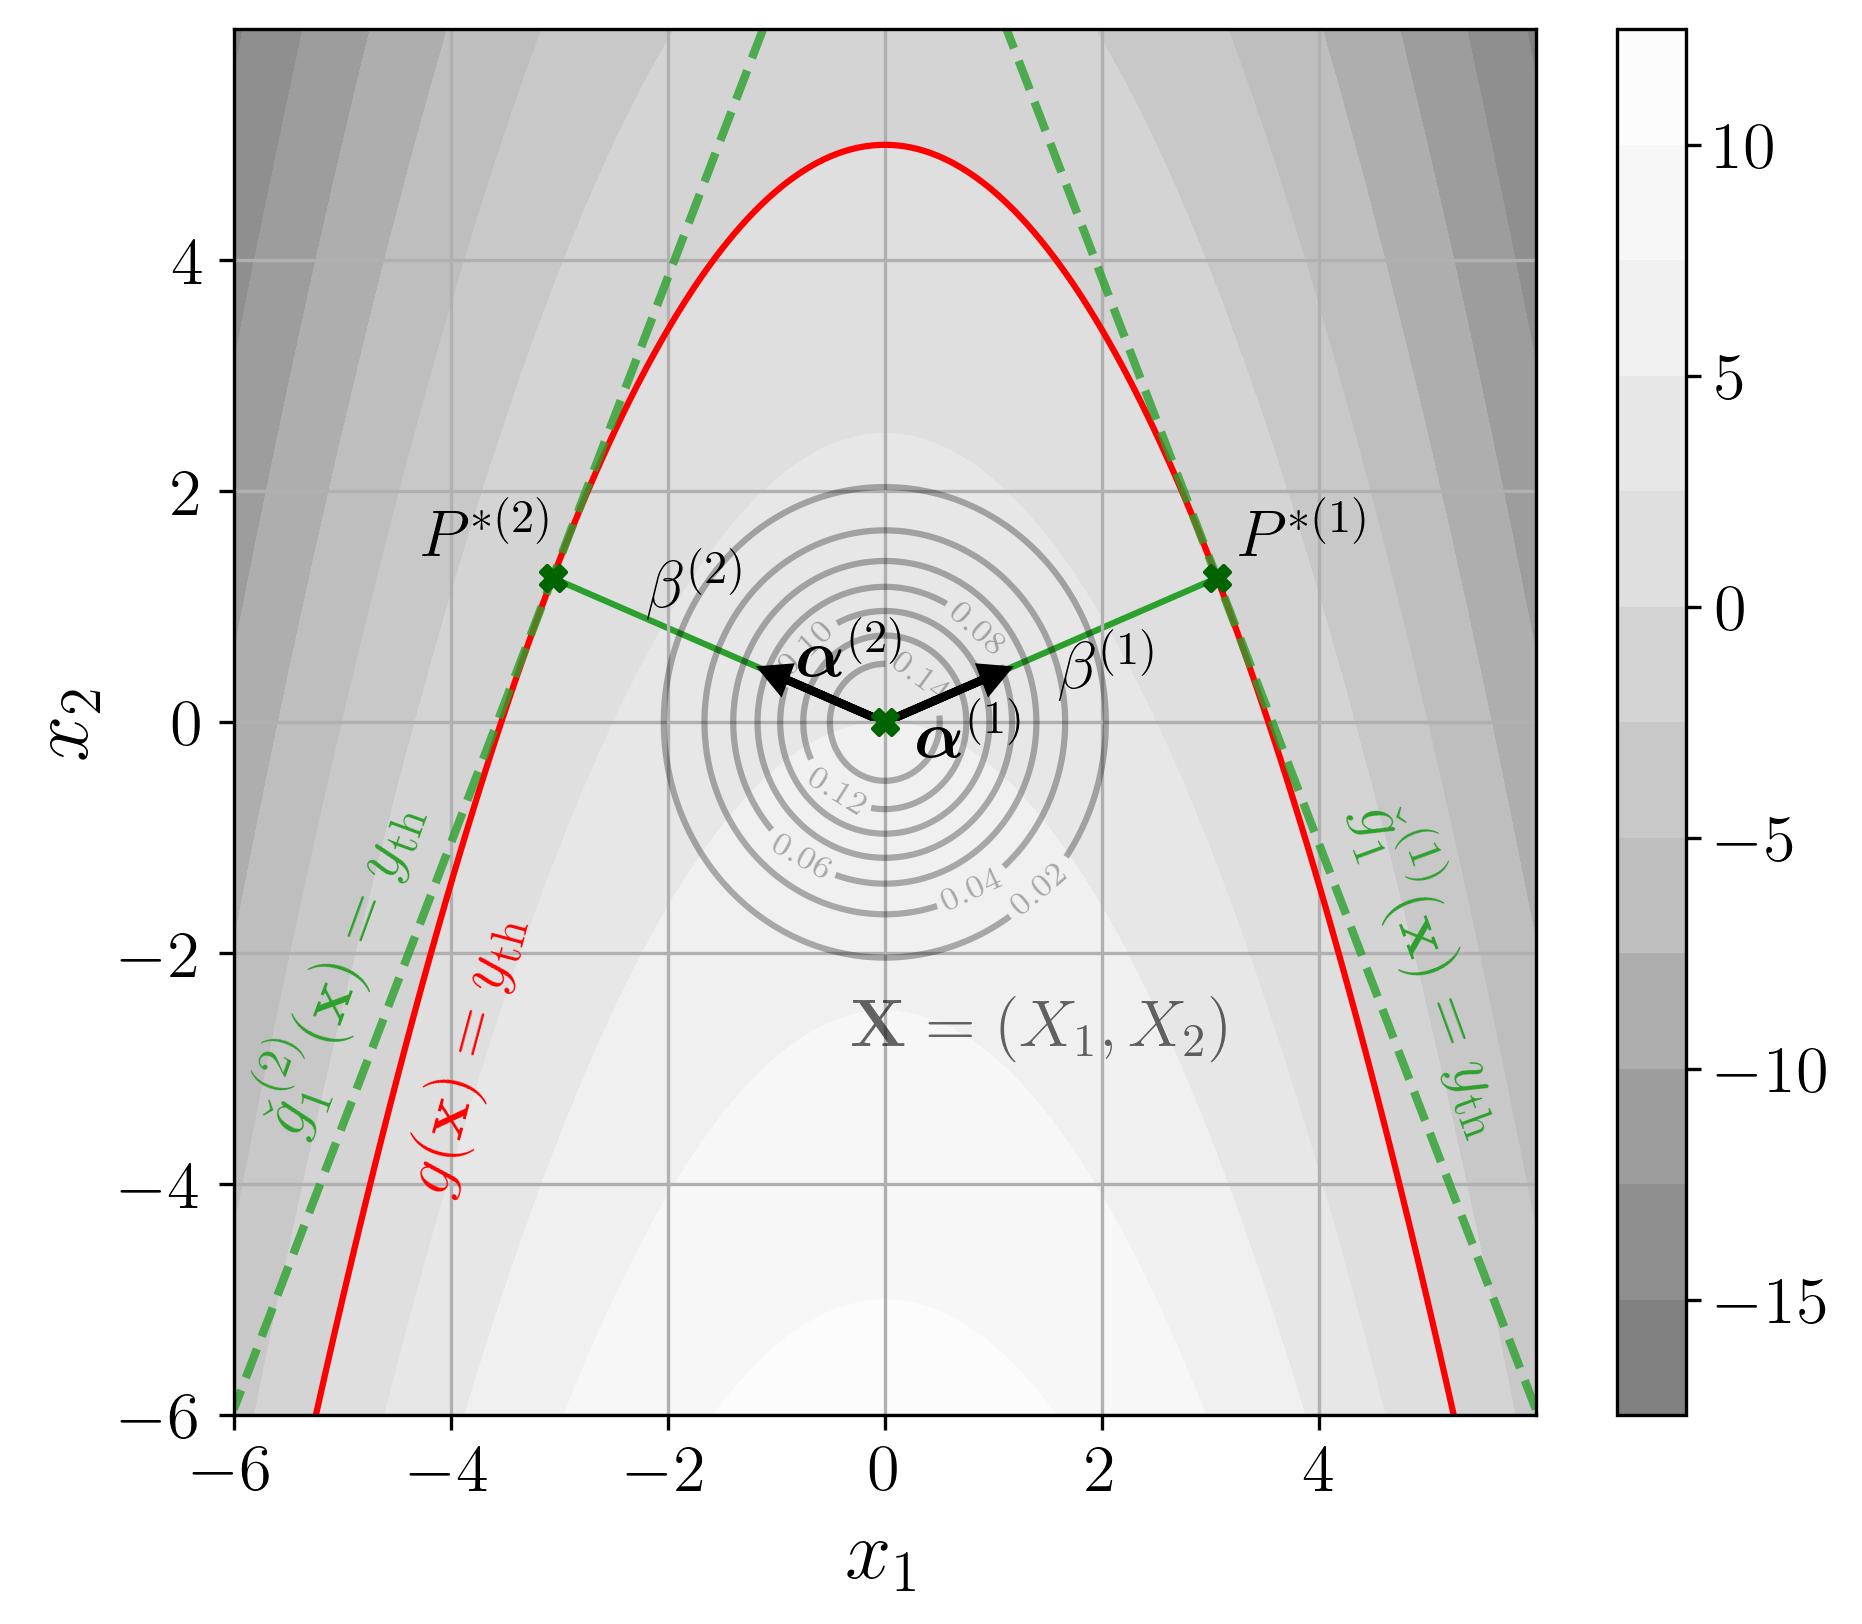
\includegraphics[width=0.48\textwidth]{../numerical_experiments/chapter1/figures/reliability_multiform.png}
    \caption{Multi-FORM approximation on an example with two MPFPs.}
    \label{fig:multi_FORM}
\end{figure}

%FORM/SORM first looks for an appropriate approximation of the limit state surface by a simple hypersurface. 
%Then, working in the standard normal space allows direct calculation of the failure probability considering the approximated limit state-function.

Overall, FORM and SORM methods deliver a very efficient approximation of small probabilities for relatively simple problems (in terms of linearity and dimension). 
For this reason, they have been widely used in the practical context of limited simulation budgets. 
\citet{straub_2014_fatigue_form} illustrates the efficiency of FORM approaches on industrial cases such as probabilistic fatigue damage. 
However, these methods present serious limits as the dimension increases (see the discussion in Chapter 1 from \citealp{chabridon_2018_thesis}). 
Additionally, their main drawback is the lack of complementary information concerning the confidence of the results. 
The textbook example illustrated in \fig{fig:multi_FORM} shows that the method might miss some significant areas of the failure domain, leading to poor estimations. 
As an alternative to approximation methods, simulation-based methods often provide the analyst with an assessment of the estimation's confidence. 


%------------------------------------------------------------%
\subsubsection{Crude Monte Carlo sampling}
%------------------------------------------------------------%
Crude Monte Carlo sampling is a universal and empirical method for uncertainty propagation. 
As introduced earlier, it relies on the pseudorandom generation of i.i.d. samples $\left\{\bx^{(i)}\right\}_{i=1}^n \simiid f_\bX$.   
The estimator is written using the indicator function applied to the LSF: 
\begin{equation}
    \pf \approx \what{\pf}^{\textrm{MC}} = \frac1n \sum_{i=1}^{n} \1_{\{\iF_\bx\}}(\bx^{(i)}).
\end{equation} 

This unbiased estimator converges towards the failure probability almost surely according to the law of large numbers. 
Once again, Monte Carlo offers an unbiased estimator, regardless of the input dimension or the regularity of the function $g(\cdot)$.   
Additionally, the variance of this estimator is given by:
\begin{equation}
    \var\left(\what{\pf}^{\textrm{MC}}\right) = \frac1n \pf \, (1 - \pf).
\end{equation} 
This variance can be used to build a confidence interval according to the central limit theorem (similarly to the ones from \eq{eq:MC_IC}). 
Because of the small scale of the quantities manipulated in rare event estimation, the estimator's coefficient of variation is also widely used: 
\begin{equation}
    \delta_{\what{\pf}^{\textrm{MC}}} = \frac{\sqrt{\var\left(\what{\pf}^{\textrm{MC}}\right)}}{\pf}
                                      = \sqrt{\frac{1 - \pf}{n \pf}}.
\end{equation}

In theory, the Monte Carlo technique presents multiple advantages for rare event estimation. 
First, this method can be applied directly in the physical space, without transformation (which is practical for complex input distributions). 
Second, it is qualified as an embarrassingly parallel method since all the numerical simulations are mutually independent. 
Finally, it offers strong convergence guarantees and complementary information on the quality of this estimation. 
These properties often make Monte Carlo sampling the reference technique in rare event estimation benchmarks. 

However, the advantages of this estimator are overshadowed by its slow convergence. 
To estimate a target failure probability $\pf=10^{-\alpha}$, 
a Monte Carlo estimation with a convergence level $\delta_{\what{\pf}^{\textrm{MC}}} = 10\%$ famously requires $n=10^{\alpha + 2}$ simulations. 
Thus, in the context of rare event estimation, Monte Carlo needs many simulations, which is often prohibitive in practice. 
This excessive simulation budget comes from the fact that the vast majority of the samples drawn from the input distribution are too far from the failure domain.


%------------------------------------------------------------%
\subsubsection{Importance sampling}
%------------------------------------------------------------%

Importance sampling (\abv{is}) is a variance reduction method, aiming at improving the performances of crude Monte Carlo sampling. 
In the context of rare event estimation, the main idea is to deliberately introduce a bias in the sampled density, shifting it towards a region of interest (here the failure domain). 
Doing so allows drawing more points in the failure domain, leading to a better estimate of the quantity.

The challenge in IS is to pick a relevant \textit{instrumental} distribution $h_\bX$ (also called \textit{auxiliary} distribution) to replace the initial distribution $f_\bX$. 
Then, by introducing the \textit{likelihood ratio} $w_\bX(\bx) = \frac{f_\bX(\bx)}{h_\bX(\bx)}$, one can rewrite $f_\bX(\bx) = w_\bX(\bx) \, h_\bX(\bx)$ and inject it in the failure probability expression: 
\begin{equation}
    \pf = \int_{\iD_\bx} \1_{\{\iF_\bx\}}(\bx) \, f_\bX(\bx) \, \dd\bx
        = \int_{\iD_\bx} \1_{\{\iF_\bx\}}(\bx) \, w_\bX(\bx) \, h_\bX(\bx) \, \dd\bx.
\end{equation}
This simple writing trick allows to integrate against the auxiliary distribution. 
With a Monte Carlo method, this task should be easier than integrating directly against the initial distribution.

The IS estimator of the failure probability is defined for a sample drawn from the auxiliary distribution such that $\left\{\bx^{(i)}\right\}_{i=1}^n \simiid h_\bX$: 
\begin{equation}
    \what{\pf}^{\mathrm{IS}} = \frac1n \sum_{i=1}^{n} \1_{\{\iF_\bx\}}(\bx^{(i)}) \, w_\bX(\bx^{(i)}).
    \label{eq:pf_IS}
\end{equation}
Similarly to Monte Carlo, this estimator is unbiased, however, its variance is defined as: 
\begin{equation}
    \var\left( \what{\pf}^{\mathrm{IS}}\right) = \frac1n \left( \E_{h_\bX}\left[\left(\1_{\{\iF_\bx\}}(\bX) \, \frac{f_\bX(\bX)}{h_\bX(\bX)}\right)^2\right] - \pf^2\right).
    \label{eq:IS_variance}
\end{equation}
The quality of the variance reduction associated with this technique fully depends on the choice of the instrumental distribution. 
In fact, IS can lead to higher variance than crude Monte Carlo when the instrumental distribution is poorly chosen \citep{owen_zhou_2000_is}. 
However, an optimal instrumental distribution $h_{\mathrm{opt}}$ theoretically gives the smallest variance by setting it equal to zero in \eq{eq:IS_variance}: 
\begin{equation}
    h_{\mathrm{opt}}(\bx) = \frac{\1_{\{\iF_\bx\}}(\bx) f_\bX(\bx)}{\pf}. 
\end{equation}
The optimal expression above is unfortunately not usable in practice since it includes the targeted quantity $\pf$. 
Considering this framework, various techniques intend to define instrumental distributions as close as possible to this theoretical result. 
An important review of the use of IS in the context of reliability analysis was proposed by \citet{tabandeh_2022_IS_review}. 

The most immediate solution is to combine the information provided by the results of FORM with IS, simply called ``FORM-IS'' \citep{melchers_1989_formis}. 
In practice, the instrumental distribution is defined as the initial distribution centered on the design point resulting from FORM. 
\fig{fig:IS_reliability} illustrates in the same two-dimensional case, the estimation by Monte Carlo and IS centered on the design point. 
On the left, it can be noticed that only a few points in red reached the failure domain. 
Such a number their number is insufficient to estimate the failure probability by Monte Carlo.  
Note that comparing the results from FORM and FORM-IS allows us to assess the nonlinearity of the LSF in the vicinity of the design point.  
This strategy is simple to implement, but it inherits the main drawbacks of FORM, such as the limits related to multiple failure areas (see the example illustrated in \fig{fig:multi_FORM}). 
Finally, other IS schemes integrate adaptive mechanisms, progressively leading the sampling towards the failure domain \citep{bugallo_2017_AIS_review}.  



\begin{figure}[ht]
    \centering
    \begin{subfigure}[b]{0.48\textwidth}
        \centering
        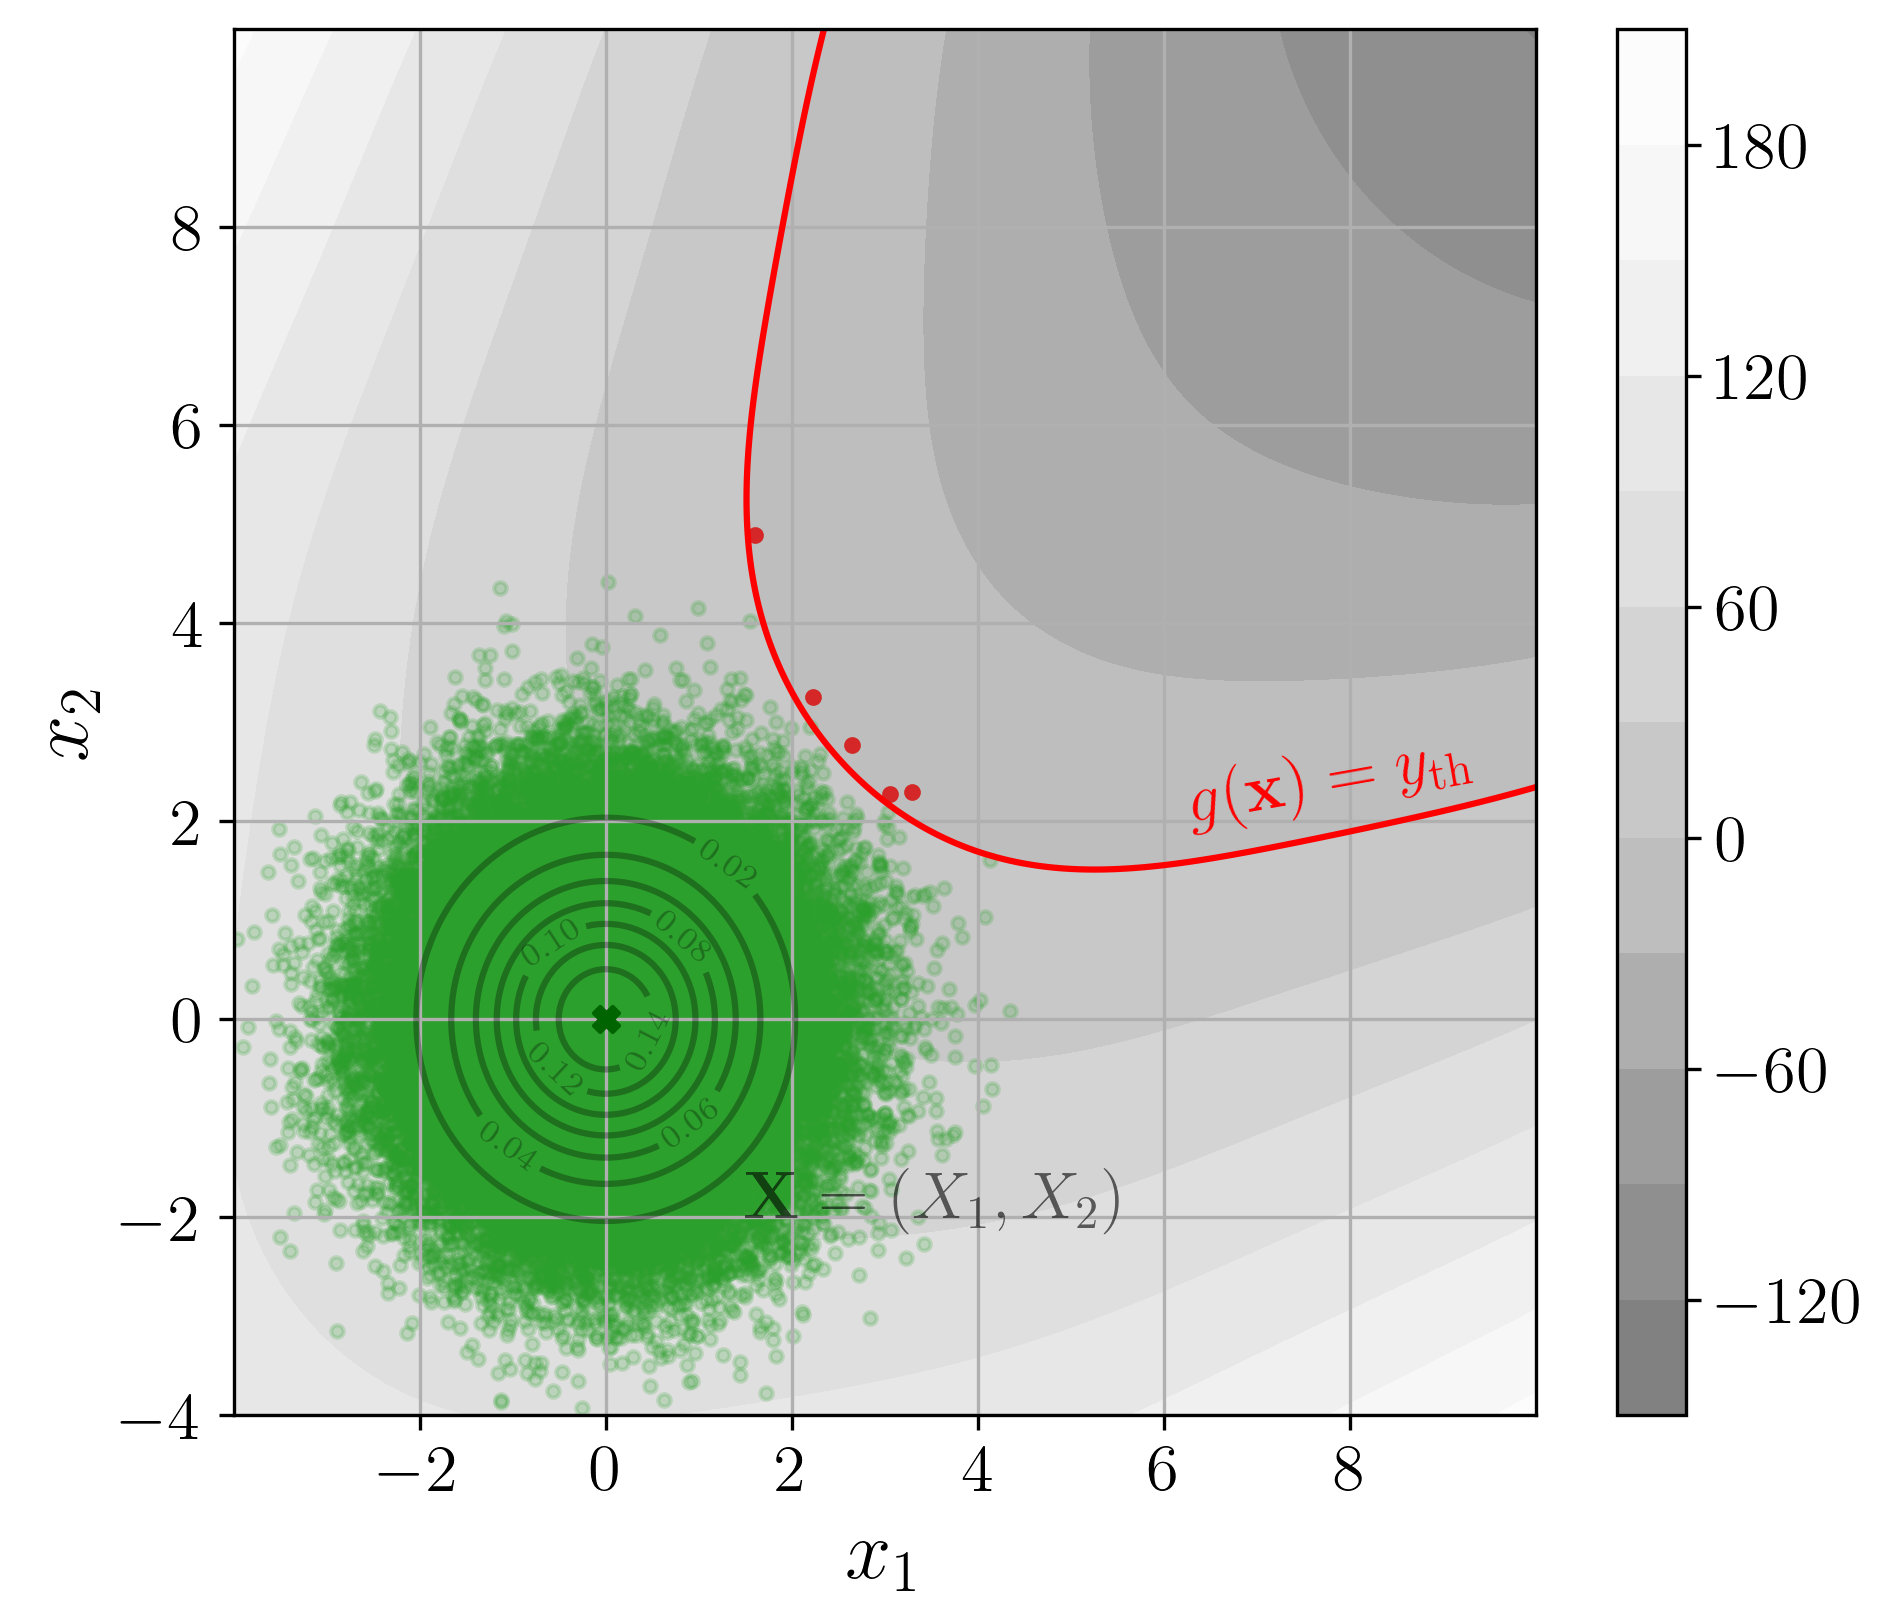
\includegraphics[width=\textwidth]{../numerical_experiments/chapter1/figures/reliability_MC_illustration.png}
        \caption{Monte Carlo ($n=10^5$).}
    \end{subfigure}
    \hfill
    \begin{subfigure}[b]{0.48\textwidth}
        \centering
        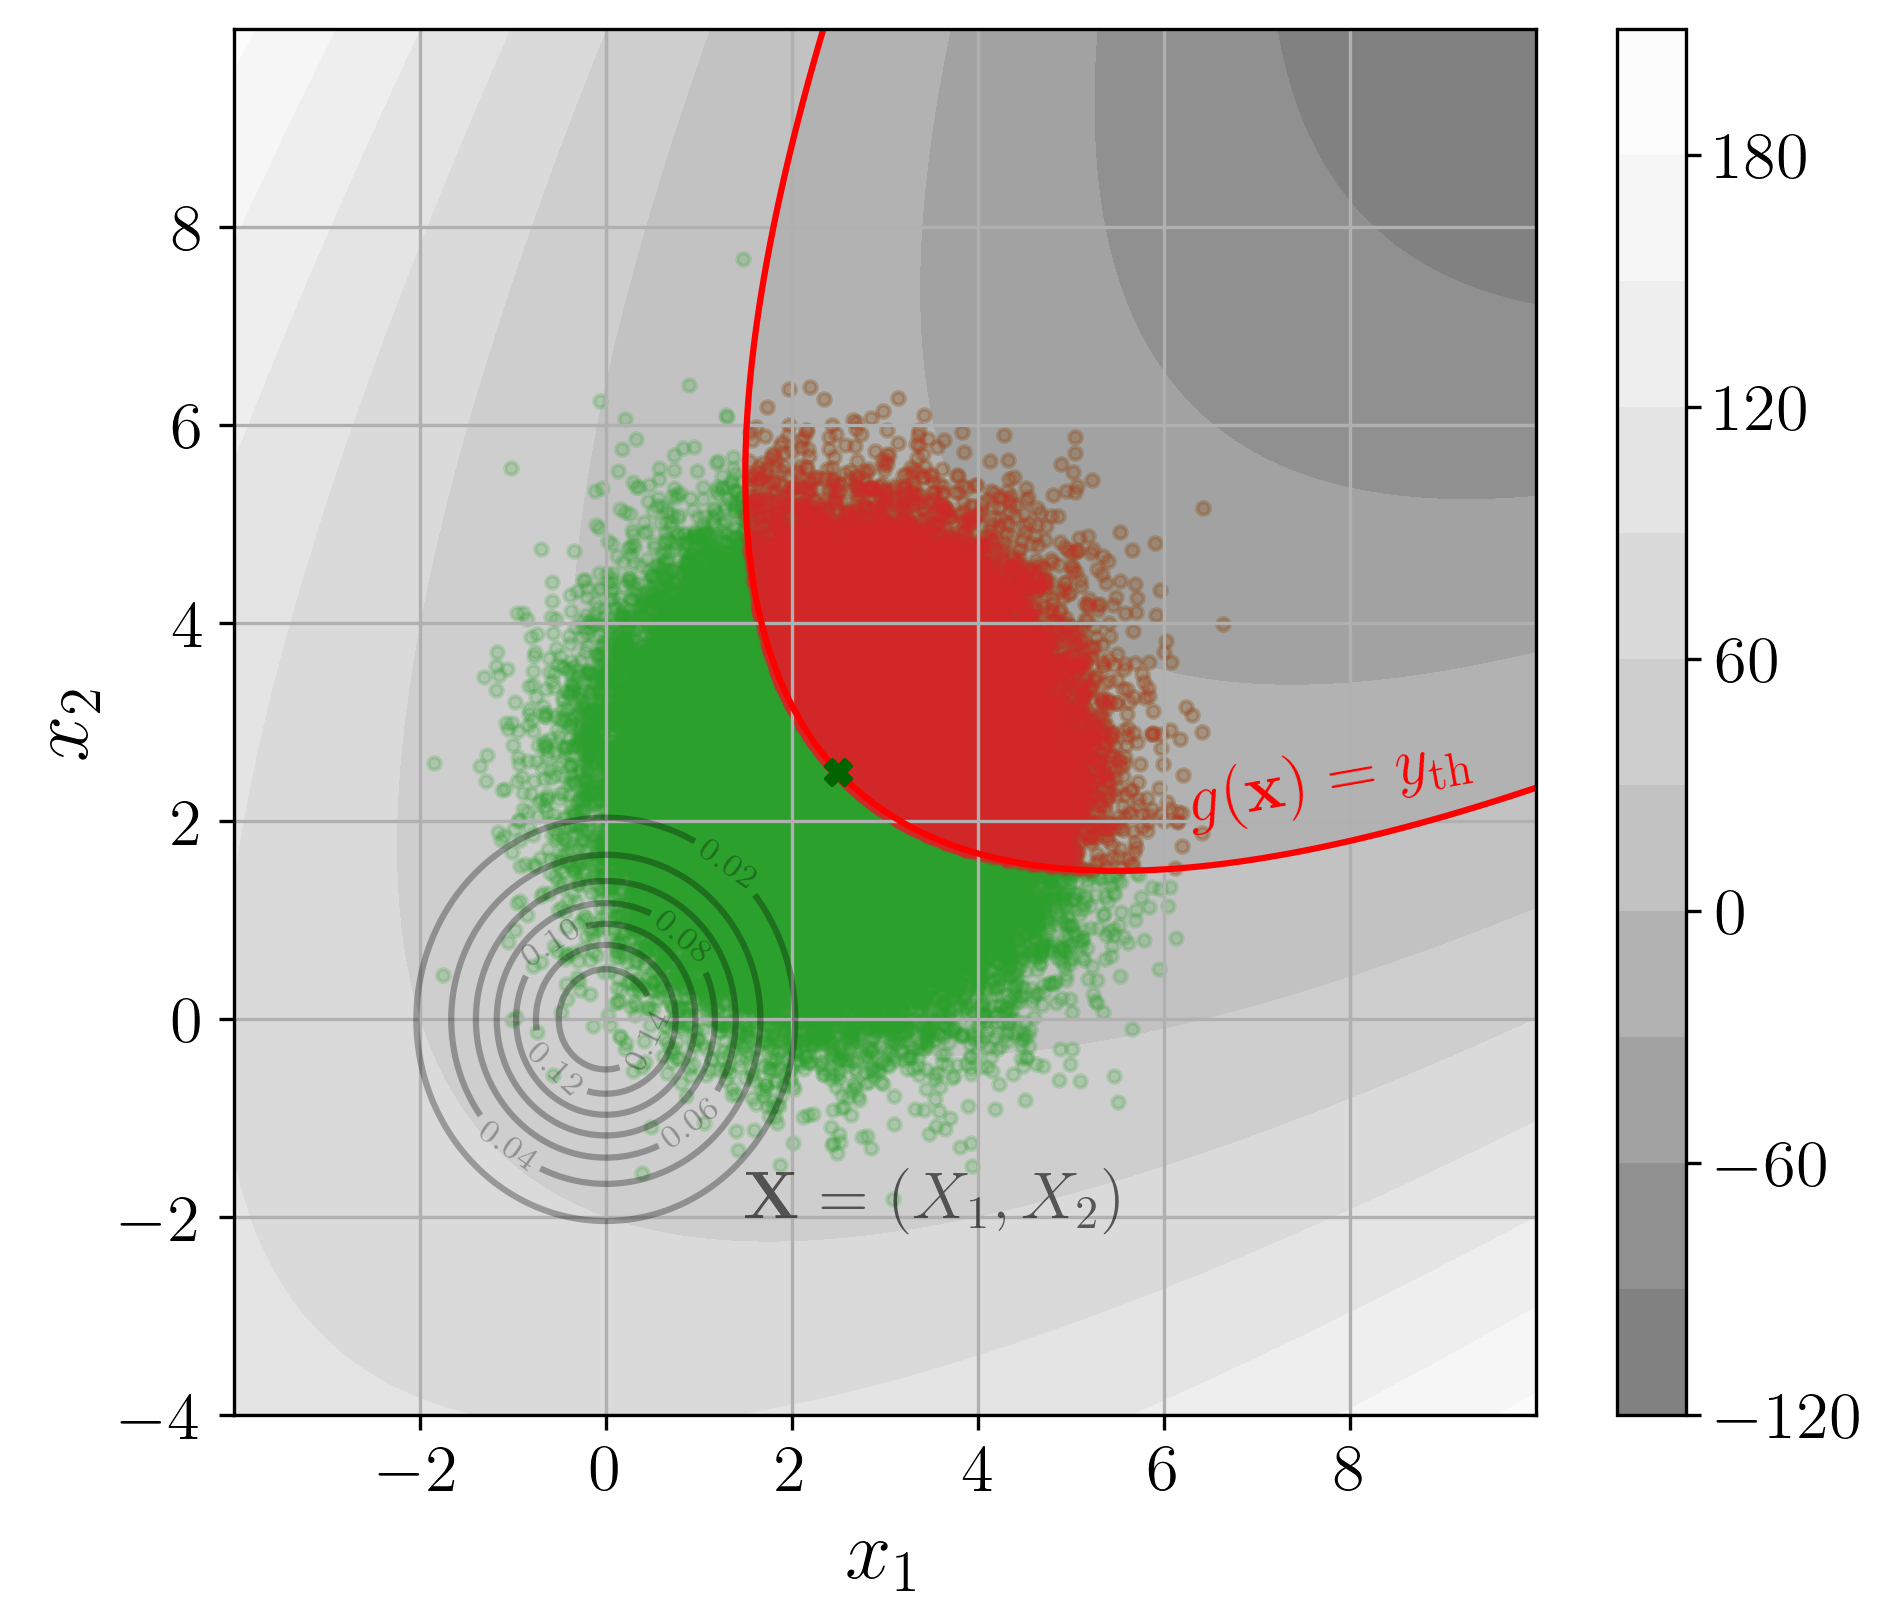
\includegraphics[width=\textwidth]{../numerical_experiments/chapter1/figures/reliability_IS_illustration.png}
        \caption{Importance sampling ($n=10^5$).}
    \end{subfigure}
    \caption{Reliability assessment by Monte Carlo and importance sampling applied to a two-dimensional problem where $g(x_1, x_2)=(x_1 - x_2) ^ 2 - 8 \, (x_1 + x_2 - 5) + \sin(x_1) + \sin(x_2)$.}
    \label{fig:IS_reliability}
\end{figure}

%------------------------------------------------------------%
\subsubsection{Adaptive importance sampling by cross-entropy}
%------------------------------------------------------------%

The \textit{cross-entropy-based adaptive importance sampling} (\abv{ceais}) is an adaptive strategy, optimizing the IS variance reduction by searching for the best instrumental distribution within a parametric family. 
Let us consider the distribution $h_{\blambda}$, belonging to the parametric family $\iH_\blambda$, defined for a set of parameters $\blambda$ in a parameter space $\iD_{\blambda} \subseteq \R^p$ as: 
\begin{equation}
    \iH_\blambda = \left\{h_\bX(\bx | \blambda) = h_{\blambda}(\bx), \, \blambda = (\lambda_1, \dots, \lambda_p) \in \iD_\blambda \subseteq \R^p\right\}.
\end{equation} 
The early work of \citet{bucher_1988_AIS} only included normal distributions to minimize the IS variance w.r.t. the parameter $\blambda$.
Using \eq{eq:IS_variance} the optimization simplifies as:
\begin{equation}
    \blambda^* = \argmin_{\blambda \in \iD_\blambda} \, \E_{h_\blambda}\left[ \1_{\{\iF_\bx\}}(\bX) \, \left(\frac{f_\bX(\bx)}{h_\blambda(\bx)}\right)^2 \right]. 
\end{equation}
However, this optimization strategy requires sampling w.r.t. the instrumental distribution at each optimization iteration, which can be avoided by using a different approach. 

The ``cross-entropy'' (CE) method \citep{rubinstein_2004_CE} uses Kullback-Leibler (\abv{kl}) divergence (introduced in Appendix~\ref{apx:B}) to optimize IS. 
The KL divergence is a dissimilarity measure between distributions, expressed between the optimal distribution $h_{\mathrm{opt}}$ and the parametric instrumental distribution $h_\blambda$: 
\begin{subequations}
    \begin{align}
        D_{\mathrm{KL}}\left(h_{\mathrm{opt}} || h_\blambda\right) &= \int_{\iD_\bx} \log \left(\frac{h_{\mathrm{opt}}(\bx)}{h_\blambda(\bx)}\right) \, h_{\mathrm{opt}}(\bx) \, \dd \bx\\
            &= \int_{\iD_\bx} \log\left(h_{\mathrm{opt}}(\bx)\right) \, h_{\mathrm{opt}}(\bx) \, \dd \bx \, - \int_{\iD_\bx} \log\left(h_\blambda(\bx)\right) \, h_{\mathrm{opt}}(\bx) \, \dd \bx.
    \label{eq:KL}
    \end{align}
\end{subequations}
\citet{rubinstein_2004_CE} simplify the expression of the optimization problem minimizing the KL divergence, which is most often convex and differentiable w.r.t. $\blambda$:  
\begin{equation}
    \blambda^* = \argmin_{\blambda \in \iD_\blambda} D_{\mathrm{KL}}\left(h_{\mathrm{opt}} || h_\blambda\right). 
\end{equation}
By injecting the expression in \eq{eq:KL}, the optimization problem simply becomes a function of an expected value over the initial density $f_\bX$:
\begin{equation}
    \blambda^* = \argmax_{\blambda \in \iD_\blambda} \int_{\iD_\bx} \log\left(h_\blambda(\bx)\right) \, h_{\mathrm{opt}}(\bx) \, \dd \bx
                = \argmax_{\blambda \in \iD_\blambda} \, \E_{f_\bX}\left[\1_{\{\iF_\bx\}}(\bX) \, \log\left(h_\blambda(\bX)\right) \right].
    \label{eq:empirical_KL}
\end{equation}
To directly estimate this expected value, the failure probability $\pf$ should not be too rare, which allows to use an empirical estimator of the expected value:
\begin{equation}
        \blambda^* = \argmax_{\blambda \in \iD_\blambda} \sum_{i=1}^{n} \1_{\{\iF_\bx\}}\left(\bx^{(i)}\right) \, \log\left(h_\blambda\left(\bx^{(i)}\right)\right) \, , \qquad
        \left\{ \bx^{(i)} \right\}_{i=1}^n \simiid f_\bX.
\end{equation}
This optimization can be solved by canceling the gradient: 
\begin{equation}
    \sum_{i=1}^{n} \1_{\{\iF_\bx\}}\left(\bx^{(i)}\right) \, \left[\nabla \log\left(h_{\blambda^*}\right)\right]\left(\bx^{(i)}\right) = \mathbf{0}.
\end{equation}
According to \citet{rubinstein_2004_CE}, this system of equations has a unique analytical solution when assuming that the instrumental distribution belongs to the ``natural exponential family''. 

However, when dealing with rare probabilities, the empirical estimation does not draw enough points in the failure domain to get an accurate estimate. 
The adaptive version of this technique, called \textit{multilevel cross-entropy}, gradually builds a set of intermediate levels, decreasing towards the failure level (equal to zero). 
By working on a set of individually less rare events, the empirical estimation in \eq{eq:empirical_KL} is made possible. 

The algorithm starts by generating and evaluating an initial sample $\left\{g\left(\bX_{[1]}^{(i)}\right)\right\}_{i=1}^n$, on which a threshold level $q_{[1]}^{\, p_0}$ is computed as the empirical $p_0$-quantile. 
Using the samples below the first threshold $q_{[1]}^{\, p_0}$, a first instrumental distribution $h_{\blambda^*_{[1]}}$ is optimized.  
At the next steps $k\in \{1, \dots, k_\# \}$, the sample $\left\{\bX_{[k]}^{(i)}\right\}_{i=1}^n$ is generated from the density $h_{\blambda^*_{[k-1]}}$ and the rest of the process repeats until the estimated threshold level becomes negative, $q_{[k_\#]}^{\, p_0} \leq 0$. 

The final instrumental density $h_{\blambda^*_{[k_{\#}]}}$ is then used for IS as defined in \eq{eq:pf_IS}: 
\begin{equation}
    \what{\pf}^{\mathrm{CE-AIS}} = \frac1n \sum_{i=1}^{n} \1_{\{g(\bx) \leq 0\}} \,
                                                 \frac{f_\bX\left(\bx^{(i)}_{[k_{\#}]}\right)}{ h_{\blambda^*_{[k_{\#}]}}\left(\bx^{(i)}_{[k_{\#}]}\right)}\, , \qquad
                                                 \left\{\bX_{[k_{\#}]}^{(i)}\right\}_{i=1}^n \simiid h_{\blambda^*_{[k_{\#}]}}.
\end{equation}

The CE-AIS algorithm is widely used in rare event estimation, as it is based on an adaptive technique while conserving the explicit IS variance given in \eq{eq:IS_variance}.  
According to \citet{rubinstein_2004_CE}, the successive instrumental distributions $h_{\blambda^*_{[k]}}$ converge towards $h_{\mathrm{opt}}$ under a few hypotheses. 
The most important one is that the optimal density must belong to the parametric family considered, which should offer enough flexibility to describe a wide range of distributions. 

When the failure domain is composed of multiple regions, different improvements of the CE-AIS have been proposed. 
\citet{kurtz_song_2013_aisce} proposed to optimize $h_{\blambda^*}$ among a mixture of Gaussian distributions. 
This method was further studied by \citet{wang_2016_aisce} and \citet{papaioannou_2019_aisce} using advanced mixtures in the standard normal space.
However, when using mixtures, the optimization problem does not have an analytical expression anymore \citep{geyer_2019_aisce}.   
In the parametric framework, the family choice leads to a complicated trade-off between optimization complexity and flexibility allowed by the family. 
%A similar mechanism is used by other IS methods, inferring the optimal instrumental density by applying kernel density estimation to the points in the failure domain. 

%------------------------------------------------------------%
\subsubsection{Nonparametric adaptive importance sampling}
%------------------------------------------------------------%
The use of multivariate kernel density estimation (\abv{kde}) to infer the IS optimal density $h_{\mathrm{opt}}$ was introduced in the context of structural reliability by \cite{ang_1992_nis}, later followed by \citet{zhang_1996_NIS}.  
Let us first present the nonparametric importance sampling from \cite{zhang_1996_NIS}, considering the instrumental density $h_{[0]}$ (for now, $h_{[0]} \neq f_\bX$), 
on which a sample $\left\{\bX_{[1]}^{(i)}\right\}_{i=1}^n$ is generated. 
A first failure probability can be roughly estimated, assuming that enough samples reach the failure domain: 
\begin{equation}
    \what{\pf}_{[1]} = \frac1n \sum_{i=1}^{n} \1_{\{g(\bx \leq 0)\}}\left(\bx^{(i)}_{[1]}\right) \frac{f_\bX\left(\bx^{(i)}_{[1]}\right)}{h_{[0]}\left(\bx^{(i)}_{[1]}\right)}
    = \frac1n \sum_{i=1}^{n} \1_{\{g(\bx) \leq 0\}}\left(\bx^{(i)}_{[1]}\right) w^{(i)}_{[1]}. 
\end{equation}
On this biased sample, another density can be fitted using KDE, using the previously defined $\what{\pf}_{[1]}$ as a normalization term: 
\begin{equation}
    \what{h}_{[1]}(\bx) = \frac{\mathrm{det}(\bH_{[1]})^{-1/2}}{n \, \what{\pf}_{[1]}} \sum_{i=1}^{n} 
            \1_{\{g(\bx) \leq 0\}}\left(\bx^{(i)}_{[1]}\right) w^{(i)}_{[1]} \, K\left(\bH_{[1]}^{-1/2} \left(\bx - \bx^{(i)}_{[1]}\right)\right)\, , 
\end{equation}
where the kernel $K$ is commonly taken as the multivariate standard Gaussian kernel with the covariance matrix $\bH$. 
The tuning of $\bH$ is usually done by minimizing an asymptotic mean integrated squared error (\abv{amise}) criterion \citep{glad_2007_kde_amise}. 
In the previous expression, the normalization constant ensures building a probability density while the weights $w^{(i)}_{[1]}$, defined above, reflect the contribution of each point to $\what{\pf}_{[1]}$.  
After performing this KDE, the estimated density can be used as instrumental density in \eq{eq:pf_IS}.

As for the CE-IS methods, the risk is that barely any points sampled from the instrumental density $h_{[0]}$ hit the failure domain, leading to poor estimates. 
\citet{zhang_1996_NIS} proposed to couple an adaptive mechanism with a nonparametric inference of the optimal density. 
This method is further referred to as \abv{nais} for \textit{nonparametric adaptive importance sampling}. 
Later, the NAIS method was adapted by \cite{Morio_RESS_2011} to the reliability analysis problem, using a similar mechanism to the CE-AIS method. 

In this framework, a series of intermediate thresholds are computed as empirical $p_0$-quantiles $q_{[1]}^{\, p_0} > \dots > q_{[k_\#]}^{\, p_0}$ of the successive importance sampling steps. 
This algorithm is initiated by setting $h_{[0]} = f_\bX$ and stops at the step $k_\#$, when  $q_{[k_\#]}^{\, p_0} < 0$.
At the step $k$, the intermediate failure probability is written as: 
\begin{equation}
    \what{\pf}_{[k]} = \frac{1}{k n} \sum_{j=1}^{k} \sum_{i=1}^{n} \1_{\{g(\bx) \leq q_{[j]}^{\, p_0}\}}\left(\bx^{(i)}_{[j]}\right) \frac{f_\bX\left(\bx^{(i)}_{[j]}\right)}{\what{h}_{[j-1]}\left(\bx^{(i)}_{[j]}\right)}
    = \frac{1}{k n} \sum_{j=1}^{k} \sum_{i=1}^{n} \1_{\{g(\bx) \leq q_{[j]}^{\, p_0}\}}\left(\bx^{(i)}_{[j]}\right) w^{(i)}_{[j]} \, , 
\end{equation}
with $\left\{\bX_{[j]}^{(i)}\right\}_{i=1}^n \simiid h_{[j-1]}$. 
Then, an intermediate instrumental density is inferred by KDE on the samples crossing the threshold $q_{[k]}^{\, p_0}$ such that:
\begin{equation}
    \what{h}_{[k+1]}(\bx) = \frac{\mathrm{det}(\bH_{[k]})^{-1/2}}{k n \, \what{\pf}_{[k]}} \sum_{j=1}^{k} \sum_{i=1}^{n} 
            \1_{\{g(\bx) \leq q_{[j]}^{\, p_0}\}}\left(\bx^{(i)}_{[j]}\right) w^{(i)}_{[j]} \, K\left(\bH_{[k]}^{-1/2} \left(\bx - \bx^{(i)}_{[j]}\right)\right).
\end{equation} 
The last instrumental density $\what{h}_{[k_{\#}]}$ is finally considered as an approximation of the optimal density for IS introduced in \eq{eq:pf_IS}: 
\begin{equation}\label{eq:pf_NAIS}
    \what{\pf}^{\mathrm{NAIS}} = \frac1n \sum_{i=1}^{n} \1_{\{g(\bx) \leq 0\}} \,
                                                 \frac{f_\bX\left(\bx^{(i)}_{[k_{\#}]}\right)}{\what{h}_{[k_{\#}]}\left(\bx^{(i)}_{[k_{\#}]}\right)} \, , \qquad
                                                 \left\{\bX_{[k_{\#}]}^{(i)}\right\}_{i=1}^n \simiid h_{k_{\#}}.
\end{equation}

Overall, NAIS offers more flexibility to infer the optimal IS density. 
This property might suit problems presenting a highly nonlinear LSF. 
Then, relying on IS still provides an expression of the estimator's variance, by adapting \eq{eq:IS_variance} to the recurrent mechanism in NAIS. 
Because this approach depends on KDE, it inherits its drawbacks. 
As discussed in \citet{Morio_RESS_2011}, tuning the KDE can create numerical issues and KDE famously suffers from the curse of dimensionality. 
In practice, the performances of NAIS significantly decrease for problems in dimensions larger than ten. 

%An algorithmic presentation of the two previous adaptive importance sampling techniques is given in Appendix D of \citet{chabridon_2018_thesis}. 


%------------------------------------------------------------%
\subsubsection{Subset simulation}
%------------------------------------------------------------%
Although the concept of ``splitting'' already existed \citep{kahn_1951_splitting}, the name of \textit{subset simulation} (\abv{ss}) was first introduced by \citet{AuBeck2001} in the structural reliability community. 
This concept was generalized as a sequential Monte Carlo method under the name of ``adaptive multilevel splitting'', as reviewed by \citet{cerou_2019_sequentialMC}. 

Subset simulation splits the failure event $\iF_{\bx}$ into an intersection of $k_\#$ intermediary events $\iF_{\bx} = \cap_{k=1}^{k_\#} \iF_{[k]}$. 
Each are nested such that $\iF_{[1]} \supset \dots \supset \iF_{[k_\#]} = \iF_{\bx}$.
The failure probability is then expressed as a product of conditional probabilities:
\begin{equation}
    \pf = \P(\iF_{\bx}) = \P(\cap_{k=1}^{k_\#} \iF_{[k]}) = \prod_{k=1}^{k_\#} \P(\iF_{[k]} | \iF_{[k-1]}).
\end{equation}

From a practical point of view, the analyst tunes the algorithm\footnotemark~by setting the intermediary probabilities $\P(\iF_{[k]} | \iF_{[k-1]}) = p_0, \forall k \in \{1, \dots, k_\# \}$. 
Then, the corresponding quantiles $q_{[1]}^{\, p_0} > \dots > q_{[k_\#]}^{\, p_0}$ are estimated for each conditional subset samples $\bX_{[k], N}$ of size $N$. 
Note that the initial quantile is estimated by crude Monte Carlo sampling on the input PDF $f_{\bX}$. 
Following conditional subset samples are generated by a \textit{Monte Carlo Markov Chain} (\abv{mcmc}) sampling technique of 
$f_{\bX}(\bx |\iF_{[k-1]})$, using as initialization points the $n= N p_0$ samples given by $\mathbf{A}_{[k], n}=\left\{\bX_{[k-1]}^{(i)} \subset \bX_{[k-1], N}| g(\bX_{[k-1]}^{(i)}) > \widehat{q}_{[k-1]}^{\, p_0} \right\}_{i=1}^n$. 
This process is repeated until an intermediary quantile becomes negative: $\widehat{q}_{[k_\#]}^{\, p_0} < 0$. 
Finally, the failure probability is estimated by:
\begin{equation}
    \widehat{\pf}^{\mathrm{SS}} = p_0^{k_\# -1} \frac1N \sum_{i=1}^n \1_{\{g(\bx) \leq 0\}} \left(\bX_{[k_\#],N}^{(i)}\right).
    \label{eq:pf_SS}
\end{equation}

\footnotetext{An algorithmic presentation of the generic subset simulation method is given in Appendix \ref{apx:C}.}

In practice, the subset sample size should be large enough to properly estimate intermediary quantiles, leading to the usual recommendation of $p_0=0.1$ \citep{AuBeck2001}. 
\fig{fig:SS_reliability} illustrates the consecutive subset samples moving towards the failure domain. 
At each step of the algorithm (corresponding to a color), a subset is generated and an intermediate quantile is estimated.   

\cite{AuBeck2001} also provide bounds to the coefficient of variation of $\widehat{\pf}^{\mathrm{SS}}$. 
The first one results from a first-order Taylor expansion of \eq{eq:pf_SS} and is often considered as an upper bound. 
The second one assumes the estimations of the conditional probabilities to be independent and tends to underestimate the coefficient of variation. 

As discussed in \citet{Papaioannou_PEM_2015}, the efficiency of the SS method often depends on the choice and tuning of the MCMC algorithm. 
The ``component-wise'' Metropolis–Hastings algorithm (or ``modified Metropolis–Hastings'') is widely used in the standard normal space for SS. 
More recently, alternative MCMC methods including physical system dynamics (e.g., Hamiltonian MCMC) showed promising results in high-dimension reliability problems \citep{papakonstantinou_2023_HMCMC}. 

The SS is a versatile method, presenting consistent performances even for rare probabilities. 
Its flexibility allows it to deal with highly nonlinear LSFs, but its drawbacks arise from the use of MCMC sampling. 
For example, the convergence of MCMC is complex to control and depends on its tuning \citep{roy_2020_mcmc_convergence}. %, in addition, the MCMC samples are dependent. 

\begin{figure}
    \centering
    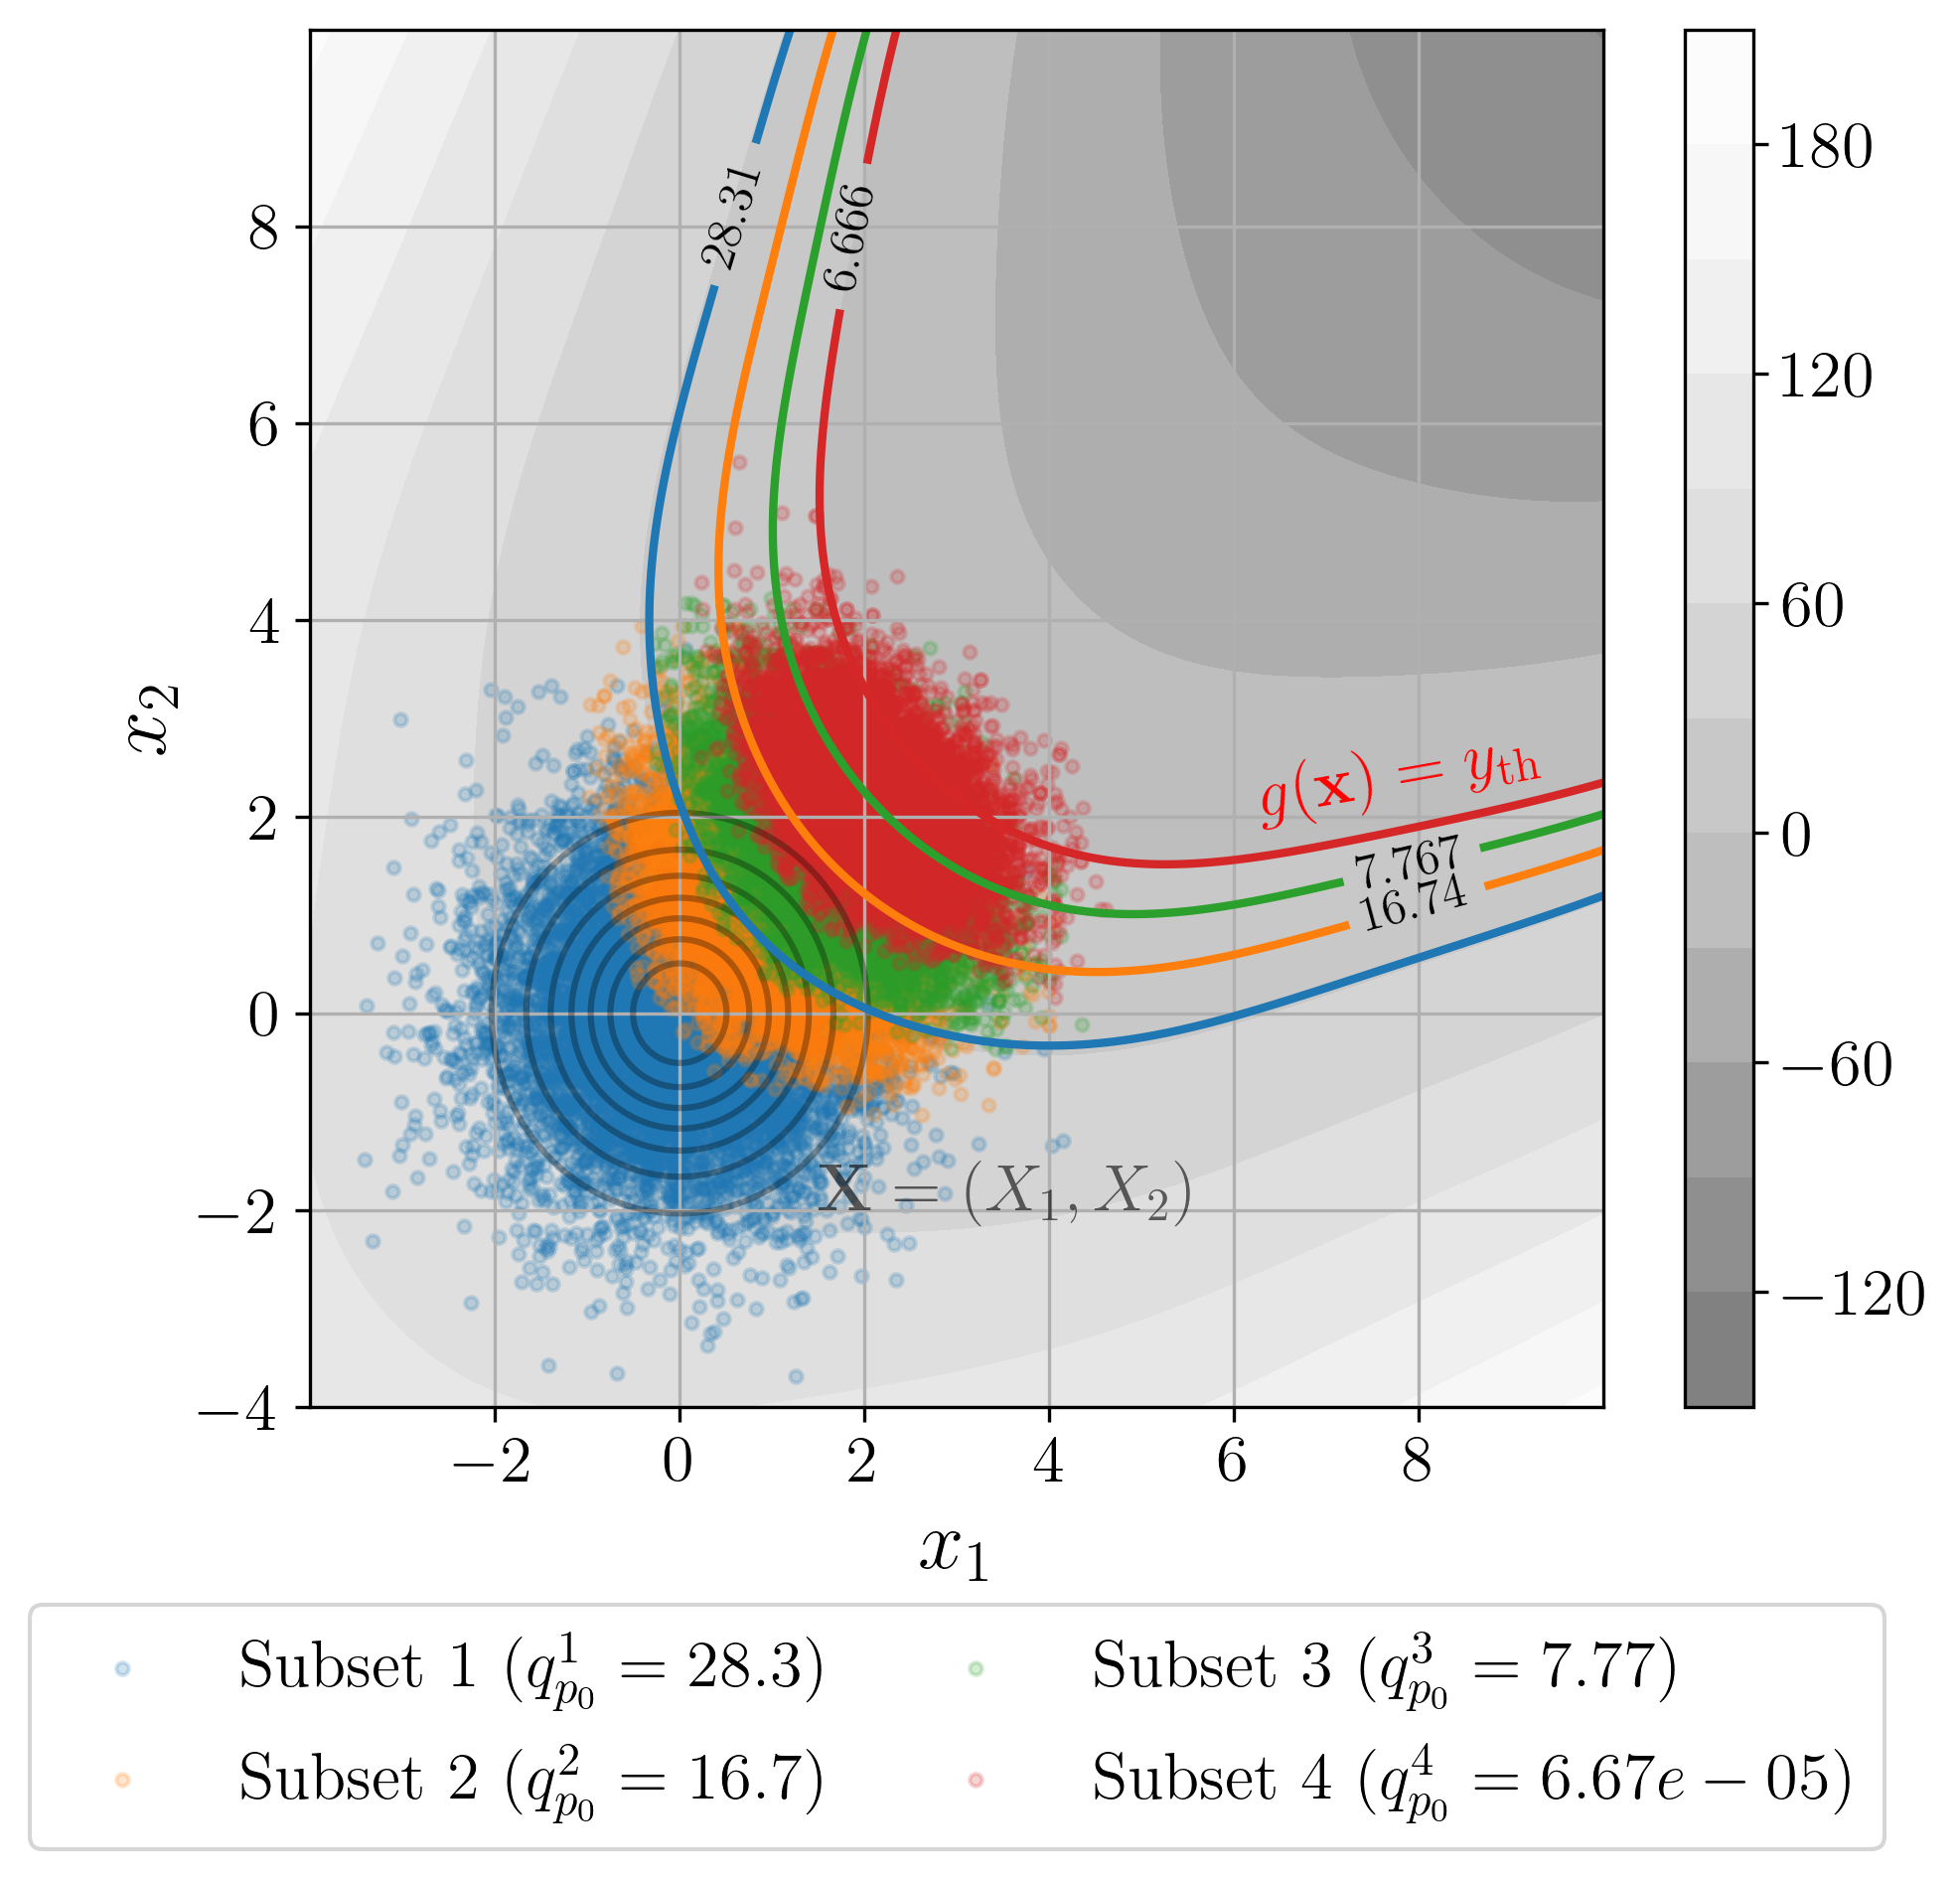
\includegraphics[width=0.5\textwidth]{../numerical_experiments/chapter1/figures/reliability_SS_illustration.png}
    \caption{Reliability assessment by subset simulation ($n=4\cdot10^4, p_0 = 0.1$) applied to a two-dimensional problem where $g(x_1, x_2)=(x_1 - x_2) ^ 2 - 8 \, (x_1 + x_2 - 5) + \sin(x_1) + \sin(x_2)$.}
    \label{fig:SS_reliability}
\end{figure}


%============================================================%
\subsection{Summary and discussion}
%============================================================%

This section introduces a generic formulation and various methods for rare event estimation. 
%Even if the problem is generic rare event estimation requires tailored solutions. 
%Depending on the properties of the problem tackled some methods might outperform others. 
However, several other methods from the field of reliability analysis are worth mentioning, such as \textit{directional sampling} \citet{bjerager_1988_directional_sampling}, \textit{line sampling} \citep{koutsourelakis_2004_line_sampling}, or more recently \textit{moving particles} \citep{walter_2015_moving_particles}. 
To go further on this topic the reader might refer to \citet{MorioBalesdent2015}, which compares the advantages and drawbacks of the most common methods and presents their algorithmic structure. 

Overall, the main properties increasing the complexity of reliability problems are related to:
\begin{itemize}
    \item the computational cost of the LSF evaluation;
    \item the nonlinearity of the LSF;
    \item the rareness of the failure event.
\end{itemize} 
In regard to the methods, the estimation is made easier by algorithms with simple tuning or allowing to work in the physical space (avoiding a possibly complex iso-probabilistic transform).
Considering all these elements the analyst may set up a sampling strategy, possibly coupled with the use of a surrogate model (further discussed in Section~\ref{sec:surrogate}). 

Nevertheless, the unified formulation of reliability analysis problems (see \ref{eq:pf}) is an opportunity for the community to share standardized benchmark problems. 
Following the well-accepted benchmark platform for optimization ``Comparing Continuous Optimizers'' (COCO) \citep{hansen_2021_coco}, an equivalent initiative was proposed for structural reliability. 
In 2019, the ``black-box reliability challenge'', was organized as a hackathon by the Dutch organization for applied scientific research (TNO) \citep{rozsas_2019_bbrc}. 
This platform proposed a large catalog of reliability problems with their respective solutions. 
Most of them were encapsulated as a Python package called \href{https://github.com/mbaudin47/otbenchmark/}{\texttt{otbenchmark}}\footnotemark$~$ \citep{fekhari_baudin_2021}, based on core \ots objects.  


\footnotetext{\url{https://github.com/mbaudin47/otbenchmark/}}

When working with computationally expensive numerical models, directly using rare event estimation methods is most often intractable. 
Many contributions were dedicated to coupling surrogate models with sampling methods for rare event estimation. 
\citet{moustapha_ss_2022} presented the results of a wide benchmark on the challenge from TNO, obtained by using surrogate models for reliability developed in the UQLab software \citep{marelli_2014_uqlab}.  

In any case, risk assessment analysts should favor the methods offering convergence guarantees over punctual performance demonstrations. 
Finally, evaluating the sensitivities and assessing the robustness of the failure probability to the input uncertainty model is a major question, which was studied within probabilistic \citep{lemaitre_2015_PLI,chabridon_2017,chabridon_2018_thesis,chabridon2021global} and extra-probabilistic \citep{ajenjo_2022_structural_safety,ajenjo_2023} frameworks. 


%%%%%%%%%%%%%%%%%%%%%%%%%%%%%%%%%%%%%%%%%%%%%%%%%%%%%%%%%%%%%%
\begin{otexample}[\href{https://github.com/efekhari27/thesis/blob/main/numerical_experiments/chapter1/reliability.ipynb}{Rare event estimation}]
    A minimal working example in Python is available in Appendix~\ref{apx:D}. 
    Figures illustrating the present section may be reproduced, using the \ots scripts available on the GitHub repository\footnotemark.  
\end{otexample}
%%%%%%%%%%%%%%%%%%%%%%%%%%%%%%%%%%%%%%%%%%%%%%%%%%%%%%%%%%%%%%
\footnotetext{\url{https://github.com/efekhari27/thesis/blob/main/numerical_experiments/chapter1/reliability.ipynb}}
%%%%%%%%%%%%%%%%%%%%%%%%%%%%%%%%%%%%%%%%%%%%%%%%%%%%%%%%%%%%%%



%============================================================%
%============================================================%
\section{Global sensitivity analysis} \label{sec:gsa}
%============================================================%
%============================================================%

After propagating uncertainties, the analyst might perform a sensitivity analysis (SA) to determine the impact of a single (or a group of random inputs) on a random output(s). 
As described earlier, this step is qualified as an inverse analysis in the general UQ framework (illustrated in \fig{fig:UQ_methodo}), in opposition to the forward uncertainty propagation step. 
In fact, the analyst studies the effect of the inputs at different scales, hence the distinction between ``local'' and ``global'' SA. 
Local SA focuses on the impact of small perturbations around nominal values of the inputs (i.e., derivative-based approaches), while
global sensitivity analysis (\abv{gsa}), typically studies the general variability (e.g., the variance) of the output. 
Two types of GSA methods exist in the literature, either proposing qualitative or quantitative approaches:  
\begin{itemize}
    \item \textit{screening methods}: determines the noninfluential variables in a UQ study (i.e., in a qualitative way);
    \item \textit{importance measures}: assess the contribution of inputs in the global variability of the output (i.e., in a quantitative way).
\end{itemize}

The global sensitivity of an output can be explained by multiple elements: the marginal effects of the inputs, their dependence, and their interactions. 
Two variables present interactions when their simultaneous effect on an output is not additive. 
%Note that SA on dependent inputs is an active field of research.

Screening methods are typically used in a statistical learning process, to drop the irrelevant variables. 
Remark that in the machine learning community, \textit{feature selection} \citep{fan_2010_feature_selection} serves the same purpose with a slight difference. 
%Screening methods usually assume the inputs to be independent while feature selection does not. 
On top of looking for the irrelevant features to the learning, feature selection investigates the redundant features.     


%============================================================%
\subsection{Screening methods}\label{sec:screening}
%============================================================%

Many UQ methods suffer from the curse of dimensionality, thankfully, high-dimensional problems often only depend on a few variables. 
This observation was formalized with the concept of \textit{effective dimension} introduced by \citet{owen_2003}. 
Screening methods allow to discriminate the noninfluential variables, which can afterward be treated as deterministic to simplify the problem.

%------------------------------------------------------------%
\subsubsection{Morris method}
%------------------------------------------------------------%

The Morris method \citep{morris_1991} is a screening method historically used in engineering applications. 
It starts by mapping the input domain $\iD_{\bX}$ into a unit hypercube $[0, 1]^d$, which is discretized as a regular grid with step $\Delta \in \R$. 
The algorithm computes local elementary sensitivity by building ``one at a time'' (OAT) local trajectories over the regular grid. 
Each OAT design starts at a random node $\bx^{(t)} = (x^{(t)}_1, \dots, x^{(t)}_j,\dots, x^{(t)}_d)$ of the grid, and moves only in one direction by an increment equal to the elementary step such that: $\bx^{(t)} + \Delta_j = (x^{(t)}_1, \dots, x^{(t)}_j + \Delta ,\dots, x^{(t)}_d)$. 
The elementary effect in the direction of the variable $j$ from an OAT trajectory $t$ is expressed as a finite difference: 
\begin{equation}
    \mathrm{EE}_j^{(t)} = \frac{g(\bx^{(t)}) - g(\bx^{(t)} + \Delta_j)}{\Delta}.
    \label{eq:eeffect}
\end{equation}

The Morris method generates $T\in\N$ OAT trajectories and computes their respective elementary effects in each direction $j$. 
To assess the global sensitivity of the function, the mean $\overline{\mathrm{EE}}_j$ and variance $\what{\var}(\mathrm{EE}_j)$ of the elementary effects are computed: 
\begin{equation}
    \overline{\mathrm{EE}}_j = \frac1n \sum_{t=1}^{T} |\mathrm{EE}_j^{(t)}|, \qquad 
    \what{\var}(\mathrm{EE}_j) = \frac{1}{n-1} \sum_{t=1}^{T} \left(\mathrm{EE}_j^{(t)} - \overline{\mathrm{EE}}_j\right)^2.
\end{equation}  


It allows to divide the variables into three categories, regardless of any regularity hypothesis on the function: 
(i) negligible effects; (ii) linear effects without interaction; and (iii) nonlinear effects with possible interactions. 
This very intuitive method quickly shows its limits as the dimension increases since it relies on a discretization of the space by a regular grid. 
Another disadvantage of this method is that it does not distinguish interactions and nonlinear effects of inputs.


%------------------------------------------------------------%
\subsubsection{Derivative-based global sensitivity measures}
%------------------------------------------------------------%

The derivative-based global sensitivity measures (DGSM) are a GSA method introduced in \citet{sobol_1995_DGSM} and further studied in \citet{kucherenko_2009_DGSM}. 
As the Morris method, it consists in computing the mean value of local derivatives of the model output w.r.t. the inputs: 
\begin{equation}
    v_j = \int_{\iD_{\bX}} \left(\frac{\partial g(\bx)}{\partial x_j}\right)^2 f_{\bX}(\bx) \, \dd \bx = \E\left[\left(\frac{\partial g(\bX)}{\partial X_j}\right)^2\right].
\end{equation}
This continuous formulation can be computed with advanced numerical integration methods such as QMC. 
The efficiency of the DGSMs for screening purposes was outlined in many papers (e.g., \citealp{kucherenko_iooss_2017}). 
Since their value depends on the probability distribution of the input, a normalized version was developed. 
The connections between DGSM and variance-based GSA measures (i.e., Sobol' indices introduced hereafter), revealed bounding properties between DGSMs and Sobol' total indices (see \citealp{roustant_2017} for further details).

%============================================================%
\subsection{Variance-based importance measures}
%============================================================%

Beyond the qualitative results from the screening methods, importance measures quantify the influence of inputs, allowing to rank the inputs according to their contribution to the output variability.  


%------------------------------------------------------------%
\subsubsection{Functional variance decomposition and Sobol' indices}
%------------------------------------------------------------%
Sobol' indices are the most popular importance measure in GSA. 
Their universality comes from the functional decomposition of the output's variance, attributing variance shares to the inputs. 
Consider a squared-integrable and measurable function $g(\cdot)$ and an independent random vector $\bX$, 
the output random variable $Y = g(\bX)$ can be decomposed, according to \citet{hoeffding_1948}, as follows: 
\begin{equation}
    Y = g_0 + \sum_{j=1}^{d} g_j(X_j) + \sum_{j<l}^{d} g_{jl}(X_j, X_l) + \dots + g_{1 \dots d}(\bX),
    \label{eq:hoeffding}
\end{equation}
with the previous terms defined according to this recurrence relation:  

\begin{subequations}
    \begin{align}
        g_0 &= \E[g(\bX)]\\
        g_j(X_j) &= \E[g(\bX) | X_j] - g_0\\
        g_{jl}(X_j, X_l) &= \E[g(\bX) | X_j, X_l] - g_j(X_j) - g_l(X_l) - g_0\\
        \dots
    \end{align}
    \label{eq:hoeffding_terms}
\end{subequations}

Several authors proved that this decomposition is unique by exploiting the orthogonality of the terms of the decomposition \citep{efron_1981,sobol_1993}. 
%\elias{add footnote for any input domain and the dependence see Chastaing these}
Therefore, this decomposition can be used to derive a functional decomposition of the variance (also called ``functional analysis of variance'' or FANOVA):
\begin{equation}
    \var(Y) = \sum_{j=1}^{d} V_j(Y)  + \sum_{j<l}^{d} V_{jl}(Y) + \dots + V_{1 \dots d}(Y)\, , 
    \label{eq:fanova}
\end{equation}
where the previous terms are defined in a recurrent way, in the same fashion as \eq{eq:hoeffding_terms}:  $V_j(Y) = \var\left(\E[Y|X_j]\right), V_{jl}(Y) =$ \allowbreak $\var\left(\E[Y|X_j, X_l]\right) - V_j(Y) - V_l(Y)$, and so on for higher order interaction terms. 
The Sobol' indices of different order are defined as normalized shares of variance. 
The \textit{first-order Sobol' index} $S_j$ quantifies the share of variance of the output only explained by the marginal $X_j$ (also called ``main effect''). 
Second order $S_{jl}$ (and higher order) Sobol' indices quantify the effect of the interactions between a group of marginals: 
\begin{subequations}
    \begin{align}
        S_j &= \frac{V_j(Y)}{\var(Y)} = \frac{\var\left(\E[Y|X_j]\right)}{\var(Y)}\\
        S_{jl} &= \frac{V_{jl}(Y)}{\var(Y)} = \frac{\var\left(\E[Y|X_j, X_l]\right) - V_j(Y) - V_l(Y)}{\var(Y)}\\
        \dots
        \label{eq:sobol_first}
    \end{align}
\end{subequations}
The generic definition of the Sobol' indices associated with a subset of inputs $A \in \mathcal{P}_d$ (see \citealp{daveiga_iooss_2021}), with $\mathcal{P}_d$ the set of all possible subsets of $\{1, \dots, d\}$, is given by:
\begin{equation}
    S_A = \frac{V_A(Y)}{\var(Y)} = \frac{\sum_{B \subset A} (-1)^{|A| - |B|} \var\left(\E[Y|X_B]\right)}{\var(Y)}\, ,
    \label{eq:sobol}
\end{equation}
where $|A|$ denotes here the cardinality of the set $A$.
By using the FANOVA in \eq{eq:fanova}, one can show that the Sobol' indices sum up to one: 
\begin{equation}
    \sum_{A \in \mathcal{P}_d} S_A = 1.
\end{equation}
The so-called \textit{closed Sobol' index} associated to a subset of inputs $A \in \mathcal{P}_d$ (equivalent to the first-order Sobol' index of $A$) is defined as: 
\begin{equation}
    S_A^{\mathrm{clos}} = \sum_{A' \subset A} S_{A'} = \frac{\var\left(\E[Y|\bX_{A}]\right)}{\var(Y)}.
    \label{eq:sobol_clos}
\end{equation}

Assessing Sobol' indices for every order becomes complex in medium to high input dimensions. 
The \textit{total Sobol' index} $S_j^T$ associated with the variable $j$, as proposed by \citet{homma_1996}, quantifies the share of output variance which is explained by all the interactions of the variable $X_j$:
\begin{equation}
    S_j^T = 1 - \frac{\var\left(\E[Y|\bX_{-j}]\right)}{\var(Y)} = \frac{\E\left[\var(Y|\bX_{-j})\right]}{\var(Y)},
    \label{eq:sobol_total}
\end{equation}
where $\bX_{-j}$ represents all the marginals from $\bX$ but $X_j$. 
This definition can also be generalized for a subset of inputs $A \in \mathcal{P}_d$, such that:
\begin{equation}
    S_A^T = 1 - S_{A^{\complement}}^{\mathrm{clos}} = 1 - \frac{\var\left(\E[Y|\bX_{A^{\complement}}]\right)}{\var(Y)} \, , 
\end{equation}
where $A^{\complement}=\mathcal{P}_d \setminus A$.
By jointly analyzing the first and total Sobol' indices, one can get an indication about the decomposition between the marginal and interaction effects. 
Note that the total indices are only equal to the first indices when the model does not present any interactions, which means that the model is purely additive.
%Moreover, the following inequalities hold: 
%\begin{equation}
%    S_j \leq 1, \qquad S_j \leq S_{T_j}, \qquad \forall j \in \{1, \dots, d\}. 
%\end{equation}

Estimating Sobol' indices can be achieved in various ways, even if historically the \textit{pick-freeze} scheme is the most popular. 
This method is based on two samples, but it often requires a prohibitive number of evaluations of the function. 
Many estimators using the pick-freeze generic scheme were developed to estimate Sobol' indices (e.g., Saltelli, Jansen, Martinez estimators), see further details in Chapter 3 of \citet{daveiga_iooss_2021}. 
Alternatively, the surrogate models can be exploited to estimate such sensitivity measures. 
Using an input-output dataset, the analyst may build a \textit{polynomial chaos expansion} (PCE) surrogate model, which gives an explicit expression of the Sobol' indices \citep{sudret_2008}. 
Authors such as \citet{marrel_2009} also studied the use of Gaussian processes for this purpose. 
  
In the case of independent inputs, the first and total Sobol' indices are a complete tool for GSA. 
The main advantage of this approach is the quantitative nature of its results, allowing to objectively compare the effect of input variables. 
When the inputs present a dependence structure, it becomes complicated to distinguish its effects from possible interactions. 
However, many authors tried to adapt Sobol' indices to this context. 
Chapter 5 of \citet{daveiga_iooss_2021} reviews four of these approaches. 
For example, \citet{mara_tarantola_2012} proposed four Sobol' indices in total, among which the ``full indices'' detect the contributions associated with the inputs' dependence. 
Note that the interpretation and estimation of this solution becomes complicated. 
Moreover, unlike the independent case, the four Sobol' indices do not divide the output variance between the inputs. 
Beyond Sobol' indices, another notable GSA method was adapted from the cooperative game theory by \citet{owen_2014_shapley}, allowing to work with dependent inputs.   

%%%%%%%%%%%%%%%%%%%%%%%%%%%%%%%%%%%%%%%%%%%%%%%%%%%%%%%%%%%%%%
\begin{otexample}[\href{https://github.com/efekhari27/thesis/blob/main/numerical_experiments/chapter1/sensitivity_analysis.ipynb}{Sobol' indices}]
    A minimal working example in Python is available in Appendix~\ref{apx:D} to assess the GSA with Sobol' indices. 
    Further scripts are also available on the GitHub repository\footnotemark.  
\end{otexample}
%%%%%%%%%%%%%%%%%%%%%%%%%%%%%%%%%%%%%%%%%%%%%%%%%%%%%%%%%%%%%%
\footnotetext{\url{https://github.com/efekhari27/thesis/blob/main/numerical_experiments/chapter1/sensitivity_analysis.ipynb}}

%------------------------------------------------------------%
\subsubsection{Shapley effects}
%------------------------------------------------------------%
The Shapley effects are an adaptation to GSA by \citet{owen_2014_shapley} of the Shapley values from the cooperative game theory \citep{shapley_1953}. 
This method is an alternative to Sobol' indices in the case of dependent inputs, for which the natural interpretation of single interaction effects no longer holds. 
In game theory, Shapley values act as a rule on how to share the value created by a team between its members (i.e., the players). 
The Shapley value allocated to the player $X_j$ is given considering the indices $-\{j\}= \{1, \dots, d\} \backslash \{j\}$:
\begin{equation}
    \varsigma_j = \sum_{A \subset -\{j\}} \binom{d-1}{|A|}^{-1} \left(\mathrm{val}(A \cup \{j\}) - \mathrm{val}(A)\right),
\end{equation}
where the value (or cost) function is denoted by $\mathrm{val}(A)$, and $A$ is a subset of $\{1, \dots, d\}$ with cardinality $|A|$. 
The Shapley effects include this concept to perform GSA by considering the variables as players and by using the closed Sobol' indices as value function: 
\begin{equation}
    \label{eq:shapley_effects}
    \mbox{Sh}_j = \sum_{A \subset -\{j\}} \binom{d-1}{|A|}^{-1} \left(S_{A\, \cup \{j\}}^{\mathrm{clos}} - S_A^{\mathrm{clos}}\right).
\end{equation}
Conceptually, this expression compares a performance defined by a cost function with or without the variable $X_j$, and averages it over all the possible combinations of inputs. 
This importance measure offers the following decomposition: 
\begin{equation}
    \sum_{j=1}^{d} \mbox{Sh}_j = 1.
\end{equation}
In the case of independent inputs, the Shapley effects present properties related to the Sobol' indices. 
The following equation (see proof in \citealp{owen_2014_shapley}) reveals that the Shapley effects equally divide the interaction effects between the implicated variables:
\begin{equation}
    S_j \leq \mbox{Sh}_j \leq S_j^T, \qquad \mbox{Sh}_j = \sum_{A \in \mathcal{P}_d, \, j \in A} \frac{S_A}{|A|}.
\end{equation}   

Unlike Sobol' indices, Shapley effects are a nonnegative allocation of output variance with equitable division of the dependence. 
This method presents an interesting alternative in the dependent case, however, estimating Shapley effects creates computational difficulties. 
A first algorithm based on permutations was proposed by \citet{song_2016_shapley}. 
Later on, surrogate models were also coupled to estimate Shapley effects, using Gaussian processes in \citet{nazben_2019_shapley}\footnotemark~ and random forests in \citet{benard_2022_shaff}. 

\footnotetext{In the vein of this work, a Python implementation using \ots is available in the GitHub repository: \\\url{https://github.com/josephmure/otshapley}.}

Shapley effects are a promising importance measure based on variance allocation. 
However, in some cases, the variance of the output distribution does not represent well its variability (e.g., multimodal distribution). 
The following section introduces another family of GSA methods based on distances between distributions.


%============================================================%
\subsection{Moment-independent importance measures}
%============================================================%
Beyond variance-based GSA, many types of distances between distributions have been used to evaluate the dependence between the input and output distributions. 
Comparing the entire distributions instead of their moments might be more robust in some cases (e.g., when the variance is a poor indicator of the variability). 
The tools used to do so are generally called \textit{dissimilarity measures} between distributions.  
Appendix \ref{apx:D} briefly introduces two families of dissimilarity measures: the class of $f$-Csisz\'{a}r divergences (e.g., the Kullback-Leibler divergence, total variation distance) and the class of integral probability metrics (e.g., Wasserstein distance, total variation distance, maximum mean discrepancy). 
%This appendix focuses on the \textit{maximum mean discrepancy} (MMD), a kernel-based dissimilarity measure between distributions with interesting estimation properties.  

Considering the probability measures $\P_{X_j}$ and $\P_{Y}$ (associated with the random variables $X_j$ and $Y$) and a dissimilarity measure $\Delta(\cdot, \cdot)$, one can define two formulations for GSA: 
\begin{itemize}
    \item directly using a dissimilarity measure to assess $\Delta(\P_Y, \P_{Y |X_j})$;
    \item building a \textit{dependence measures} evaluating $\Delta(\P_{(X_j, Y)}, \P_{X_j} \otimes \P_Y)$.
\end{itemize}

The first approach was studied in association with $f$-divergences in \citet{daveiga_2015,rahman_2016}. 
However, some $f$-divergences introduce estimation issues, and the resulting importance measures do not propose a FANOVA.  
Using kernel-based integral probability metrics such as the maximum mean discrepancy (\abv{mmd}), an alternative importance measure was proposed.  
The following section presents the \textit{Hilbert-Schmidt independence criterion} (\abv{hsic}), which was initially introduced by \citet{gretton_2006} to detect the dependence, and later adapted as a dependence measure in GSA by \citet{daveiga_2015}. 


%------------------------------------------------------------%
\subsubsection{Hilbert-Schmidt independence criterion}
%------------------------------------------------------------%

Let us first recall the definition of the maximum mean discrepancy (further discussed in Appendix \ref{apx:D}). 
This distance between two probability distributions $\pi$ and $\zeta$ can be defined as the worst-case error for any function within a unit ball of a function space $\iH$, which is a Reproducing kernel Hilbert space (\abv{rkhs}):
\begin{equation}
    \MMD(\pi, \zeta) = \sup_{\lVert g \lVert_{\iH(k)} \leq 1} \left | \int_{\iD_{\bX}} g(\bx) \dd \pi(\bx) - \int_{\iD_{\bX}} g(\bx) \dd \zeta(\bx) \right | 
    %= \left\lVert P_{\pi}(\bx) - P_{\zeta}(\bx) \right\lVert_{\iH(k)}.
    \label{eq:mmd_chapter1}  
\end{equation}
This quantity is a distance in the RKHS by taking a characteristic kernel (e.g., the Gaussian or Mat\'{e}rn kernel). 
After a calculation developed in Appendix \ref{apx:D}, an unbiased one-sample estimator of the squared-MMD was proposed by \citet{gretton_2006}, 
with a convergence rate of $\mathcal{O}(n^{-1/2})$ in probability. 
Considering the two-samples $\left\{\pi^{(i)}\right\}_{i=1}^n \sim \pi$ and $\left\{\zeta^{(j)}\right\}_{j=1}^n \sim \zeta$: 
\begin{equation}
    \what{\MMD}^2(\pi, \zeta) = \frac{1}{n (n-1)} \sum_{i=1}^{n} \sum_{j \neq i}^{n} 
                                k\left(\pi^{(i)}, \pi^{(j)}\right) - k\left(\pi^{(i)}, \zeta^{(j)}\right) - k\left(\zeta^{(i)}, \pi^{(j)}\right) + k\left(\zeta^{(i)}, \zeta^{(j)}\right) \, , 
\label{eq:mmd_ustat}
\end{equation}
where $k(\cdot, cdot)$ is a symmetric and positive definite kernel with specific properties (see Appendix~\ref{apx:B} for further details).

In the context of GSA, the first option is to directly use this dissimilarity measure to define the following unnormalized index: 
\begin{equation}
    S_j^{\MMD} = \MMD(\P_Y, \P_{Y |X_j}). 
    \label{eq:mmd_gsa}
\end{equation}
\citet{daveiga_2021_kernel_ANOVA} remarked that the unormalized first-order Sobol' indices are recovered by taking the linear kernel on the output, such that $k_{Y}(y, y')=y\, y'$. 
Using this non-characteristic kernel (see the definition in Appendix \ref{apx:D}) brings us back to a moment-dependent importance measure. 

Alternatively, the second option consists in considering a couple of random variables $(X_j, Y)$, with probability distributions $\P_{X_j}$ and $\P_Y$, and assuming the RKHS $\iH$  
induced by the tensor product kernel $k((x_j, y), (x_j', y')) = k_{X_j}(x_j, x_j') k_{Y}(y_j, y_j')$. 
The \textit{Hilbert-Schmidt independence criterion} (HSIC) measures the dependence between $\P_{X_j}$ and $\P_Y$ by expressing the MMD between $\P_{(X_j, Y)}$ and $\P_{X_j} \otimes \P_{Y}$ and is given by: 
\begin{equation}
    \mathrm{HSIC}(X_j, Y) = \MMD^2(\P_{(X_j, Y)}, \P_{X_j} \otimes \P_{Y}).
    \label{eq:hsic}
\end{equation}
This technique showed very good results for screening, and corresponding independence tests were studied for screening in \citet{delozzo_2016_hsic_test}. 

\citet{daveiga_2021_kernel_ANOVA} proposed the functional decomposition of the two indices defined in \eq{eq:mmd_gsa} and \eq{eq:hsic}, allowing to develop their respective normalized versions. 
Note that the HSIC decomposition requires a specific hypothesis on the structure of the kernel associated with the inputs. 



%============================================================%
\subsection{Summary and discussion}
%============================================================%

This section introduces the GSA methods commonly used in UQ. 
Either to reduce the dimension of a problem (screening) or to quantify the influence of inputs (with importance measures), GSA improves the understanding of a UQ study.   
As for other steps of the generic UQ methodology, GSA is made more complicated for computationally costly simulation models, hence the use of surrogate models. 
Additionally, the dependence between inputs still represents an important limit to interpreting GSA results. 

Alongside rare event estimation, some literature is dedicated to the influence of random inputs on such tail statistics. 
The sensitivity is no longer qualified as ``global'' but becomes ``goal-oriented''. 
In the field of structural reliability, an overview of the reliability-oriented sensitivity analysis methods is presented in \citet{chabridon_2018_thesis}. 
Several techniques derive from rare event estimation (e.g., the reinterpretation of the FORM importance factors by \citealp{papaioannou_2021_rosa_form}), or were adapted from GSA, like Sobol' indices \citep{wei_2012_rosa,chabridon_2018_thesis,perrin_2019_rosa,ehre_2020_rosa}, Target-HSIC \citep{marrel_chabridon_2021}, or Shapley effects \citep{ilidrissi_2021_rosa}.  

Finally, sensitivity analysis may describe the effects of random inputs on the variation of the output, however, this study is done by assuming a model on the input uncertainties. 
The role of a regulatory agency auditing a UQ approach for certification (i.e., a nuclear safety authority), might be to challenge the way to model the uncertainties on the inputs.  
In this case, various tools for \textit{robustness analysis} exist to quantify the impact of mispecifying the random inputs on the quantity of interest studied. 
Among the methods to perturbate uncertainty models, some remain in the probabilistic framework, such as the ``perturbed-law based indices'' (\abv{pli}) \citep{lemaitre_2015_PLI,iooss_2022_pli}, while other rely on extra-probabilistic methods \citep{ajenjo_2022_structural_safety}. 




%============================================================%
%============================================================%
\section{Surrogate modeling} \label{sec:surrogate}
%============================================================%
%============================================================%

%============================================================%
\subsection{Common framework}
%============================================================%

The aim of \textit{surrogate modeling} (or metamodeling) is to build a cheap-to-call statistical model, 
denoted by $\wg_n(\cdot)$, to replace a costly numerical model $g(\cdot)$ over the input domain $\iD_{\bX}$. 
To do so, statistical learning is performed on a finite number of observations of the costly function $g$. 
When manipulating computationally expensive simulations, the sample size can be limited (i.e., in a small-data context). 
This $n$-sized sample is usually called \textit{learning set} and written: 
\begin{equation}
    \left\{\bX_n, \by_n\right\} = \left\{\bx^{(i)}, y^{(i)}\right\}_{i=1}^n
                                = \left\{\bx^{(i)}, g\left(\bx^{(i)}\right)\right\}_{i=1}^n.    
\end{equation}

A very large catalog of regression methods exists. 
Here is a list of the most encountered ones in the field of UQ:
generalized linear regression, polynomial chaos expansion (PCE) \citep{soize_2004, blatman_2011}, support vector machine \citep{vapnik_1995}, 
Gaussian processes (GP) \citep{rasmussen_2006}, low-rank tensor approximations \citep{grasedyck_2013}, and artificial neural network \citep{tibshirani_2009}.
The following section will provide a short focus on GP regression. %\elias{Add BST's table including names/shape/parameters/reference?}

Validating the accuracy and precision of a surrogate model is a crucial step to guarantee its fidelity with regard to the numerical model. 
When an $m$-sized input-output set is dedicated to validating the surrogate model, independently of the learning set, 
it is called \textit{test set} and denoted by $\left\{\bX_m, \by_m\right\} = \left\{\bx^{(i)}, g\left(\bx^{(i)}\right)\right\}_{i=1}^m$. 
Note that the analyst may work in two different frameworks, affecting the regression and validation method's choice: 
\begin{itemize}
    \item The given-data context: only using a fixed input-output dataset to build and validate the surrogate model. 
    \item The computer experiment context: allowing to generate simulated data points (often at a certain cost).
\end{itemize}

Validating surrogate models in a small-data context appears to be a challenge. 
Multiple validation criteria and techniques exist. 
The \textit{regression coefficient}, denoted by $R^2$, is the first validation metric that can be directly computed on the learning set:
\begin{equation}
    \mathrm{R}^2(\wg_n) = 1 - \frac{ \sum_{i=1}^n  \left(y(\bx^{(i)}) - \wg(\bx^{(i)})\right)^2}{\sum_{i=1}^n \left(y(\bx^{(i)})-\overline{\by}_n\right)^2}\,,
\end{equation}
where $\overline{y}_n=(1/n)\,\sum_{i=1}^n y^{(i)}$ denotes the empirical mean of the observations in the learning sample. 
However, such metrics are not relevant for every regression method (typically, the interpolant methods have an $R^2=1$). 
The \textit{predictivity coefficient} \citep{NashS70} is another criteria defined as a normalized \textit{integrated square error} (\abv{ise}): 
\begin{equation}
    \mathrm{Q}^2(\wg_n) = 1 - \frac{\ISE(\wg_n)}{\var(g(\bX))}, 
\end{equation} 
where 
\begin{equation}
    \ISE(\wg_n) = \int_{\iD_{\bX}} \left(g(\bx) - \wg(\bx)\right)^2 \, \ddx, \qquad
    \var(g(\bX)) = \int_{\iD_{\bX}} \left(g(\bx) - \int_{\iD_{\bX}} g(\bx)\, \ddx' \right)^2 \, \ddx.
\end{equation}
This quantity can be estimated on a test set $\left\{\bX_m, \by_m\right\}$ as follows: 
\begin{equation}
    \what{\mathrm{Q}}^2(\wg_n) = 1 - \frac{ \sum_{i=1}^m  \left(y(\bx^{(i)}) - \wg(\bx^{(i)})\right)^2}{\sum_{i=1}^m \left(y(\bx^{(i)}) - \overline{\by}_m\right)^2}\,.
\end{equation}
Note that for either criterion, the closer to one, the better the quality of the fit. 

Validating a surrogate model with an independent test set is sometimes called \textit{holdout} validation.
In a small-data context, dedicating an independent test set to validation might be impossible.
Then, \textit{cross-validation} is a generic estimation strategy allowing one to learn and test on the same sample. 
The most common cross-validation method is the \textit{$k$-fold} validation, illustrated in \fig{fig:kfold}. 
The idea is first to split the $n$-sized dataset into several equal parts, called ``folds''. 
A first surrogate can be fitted on the entire datasets but the first fold, on which a validation criterion is estimated (i.e., performance metric). 
The operation is repeated for each fold, providing a virtual validation of the entire dataset. 
Leave-One-Out validation (\abv{loo}) is an extreme case of $k$-fold cross-validation, for which $k=n-1$. 
Note that multiple variations of these methods exist, for example by adding a permutation or shuffling step. 
The ``bagging'' validation method (for ``bootstrap aggregating'') consists of shuffled cross-validation repeated many times \citep{breiman_1996_bagging}. 

%\elias{Should we mention bootstrap aggregating (bagging): ensemble meta-algorithm improving the stability and accuracy of machine learning algorithms}

\begin{figure}[ht]
    \centering
    \begin{tikzpicture}
        \matrix (M) [matrix of nodes,
            nodes={minimum height = 4mm, minimum width = 1.2cm, outer sep=0, anchor=center, draw},
            column 1/.style={nodes={draw=none}}, column 6/.style={nodes={draw=none}},
            row sep=1pt, column sep=-\pgflinewidth, nodes in empty cells,
            e/.style={fill=orange!20}
          ]
          {
            \textit{Test set}: 1\textsuperscript{st} fold & |[e]| & & & & $\Rightarrow$ Performance metric \#1: $\what{Q}^2_1$\\
            \textit{Test set}: 2\textsuperscript{nd} fold & & |[e]| & & & $\Rightarrow$ Performance metric \#2: $\what{Q}^2_2$\\
            \textit{Test set}: 3\textsuperscript{rd} fold & & & |[e]| & & $\Rightarrow$ Performance metric \#3: $\what{Q}^2_3$\\
            \textit{Test set}: 4\textsuperscript{th} fold & & & & |[e]| & $\Rightarrow$ Performance metric \#4: $\what{Q}^2_4$\\
          };
          \draw (M-1-2.north west) ++(0,2mm) coordinate (LT) edge[|<->|, >= latex]
                     node[above]{Total data available} (LT-|M-1-5.north east);
      \end{tikzpicture}
      \caption{Illustration of a $k$-fold cross-validation (with $k=4$).} 
      \label{fig:kfold}
\end{figure}



%============================================================%
\subsection{Focus on Gaussian process regression}
%============================================================%

In this subsection, a particular focus is dedicated to GP regression which will be useful in the following chapters (GP regression is also called ``Kriging'' after the mining engineer D.G. Krige). 
GP has been widely used as a regression method in UQ since the seminal paper of \citep{sacks_1989}, for their performance, flexibility and their associated confidence model. 
In a small-data context, the way of placing the few points forming the surrogate's learning set is critical. 
Intuitively, to build a versatile surrogate model, the learning set should collect information over the entire domain uniformly. 
This is why space-filling designs of experiments are commonly used to build learning sets \citep{fang_li_2006}. 
In practice, QMC and optimized LHS design introduced in Section~\ref{sec:central_propagation} are widely used.  

Considering a learning set $\left\{\bX_n, \by_n\right\}$, the goal is to approximate the function $g(\cdot)$ by a scalar GP conditioned on a set of observations $\by_n = \left\{g\left(\bx^{(i)}\right)\right\}_{i=1}^n$. 
Let us first define a prior structure $G$ on the function approximating $g(\cdot)$, taken as a GP with a mean function $m(\cdot)$ and covariance function $k(\cdot, \cdot)$:  
\begin{equation}
    G \sim \GP(m(\cdot), k(\cdot, \cdot)),
\end{equation} 
with: 
\begin{itemize}
    \item a \textit{trend model}: $~m(\bx) = \mathbf{f}(\bx)\TT \bbeta$, composed of a functional basis with $p \in \N^*$ components $\mathbf{f} = \left(f_1, \dots, f_p\right)\TT$ and a vector of coefficients 
    $\bbeta = \left(\beta_1, \dots, \beta_p\right)\TT$;
    \item a \textit{covariance model}: $~k(\bx, \bx')$, usually taken stationary, such that $k(\bx, \bx') = \sigma^2 k_{\mathrm{s}}(\bx - \bx', \btheta)$ with $\sigma^2>0$ and $\btheta \in \R^d_+$.
\end{itemize}
The trend model of a GP defines its general tendency, while the covariance model influences its regularity. 
GP regression takes different names depending on the knowledge of the trend model. 
It is called ``simple Kriging'' when the trend is fully known, ``ordinary Kriging'' when the trend is unknown but supposed constant and ``universal Kriging'' otherwise. 
%Note that \cite{schobi_2015} introduced a hybrid method named PC-Kriging setting a PCE as the trend of a Kriging model. %\elias{paper PLS-Kriging from Onera 2015.}

To ease the presentation, let us first assume the hyperparameters $(\sigma^2, \btheta)$ are fully known and the trend is zero: $\bbeta = \textbf{0}$. 
At a given point $\bx \in \iD_\bX$ the realization of the GP is a Gaussian random variable, i.e.,  $G(\bx) \sim \iN(m(\bx), k(\bx, \bx))$. 
Working with Gaussian variables allows us to easily write conditioning formulas between $G(\bx)$ and the observations $\by_n$. 
This Gaussian variable $G(\bx)$ conditioned on the observations $\by_n$ is sometimes called the ``conditional posterior'' $G_n(\bx) = (G(\bx) | \by_n) \sim \iN(\eta_n(\bx), s_n^2(\bx))$. 
The well-known ``Kriging equations'' (see e.g., \citealp{rasmussen_2006}) offer the explicit expression of the parameters of this distribution:
\begin{equation}
    \left\{
    \begin{array}{ll}
        \eta_n(\bx) &= \bk\TT(\bx) \bK^{-1} \by_n\\
        s_n^2(\bx) &= k(\bx, \bx) - \bk\TT(\bx) \bK^{-1} \bk(\bx) 
    \end{array}\, ,
\right.
\label{eq:kriging}
\end{equation}
where $\bk(\bx)$ is the column vector of the covariance kernel evaluations $[k(\bx, \bx^{(1)}), \dots,\allowbreak k(\bx, \bx^{(n)})]$ and $\bK$ is the $(n \times n)$ 
variance-covariance matrix such that the $(i, j)$-element is $\left\{\bK \right\}_{i, j}=k(\bx^{(i)}, \bx^{(j)})$.

In practice, the surrogate model is defined by the \textit{predictor} function $\eta_n(\cdot)$. 
This regression model provides remarkable complementary information with the \textit{Kriging variance} $s_n^2(\bx)$, reaching zero at the learning points. 
Let us remark that the Kriging variance fully depends on the covariance model (defined by its parametric structure and hyperparameters). 
In practice, the hyperparameters are unknown, therefore, their estimation is a key step in the construction of a Kriging model. 
This estimation can be done using different approaches, most commonly using maximum likelihood estimation (\abv{mle}) or cross-validation.

The illustration in \fig{fig:kriging_1D} is a typical one-dimensional representation of an ordinary Kriging model. 
The mean of the conditioned process is plotted in red while its variability is represented by the many trajectories drawn on the process. 
In the simplest framework, the Kriging model exactly interpolates the observations (black crosses). 

\begin{figure}[ht]
    \centering
    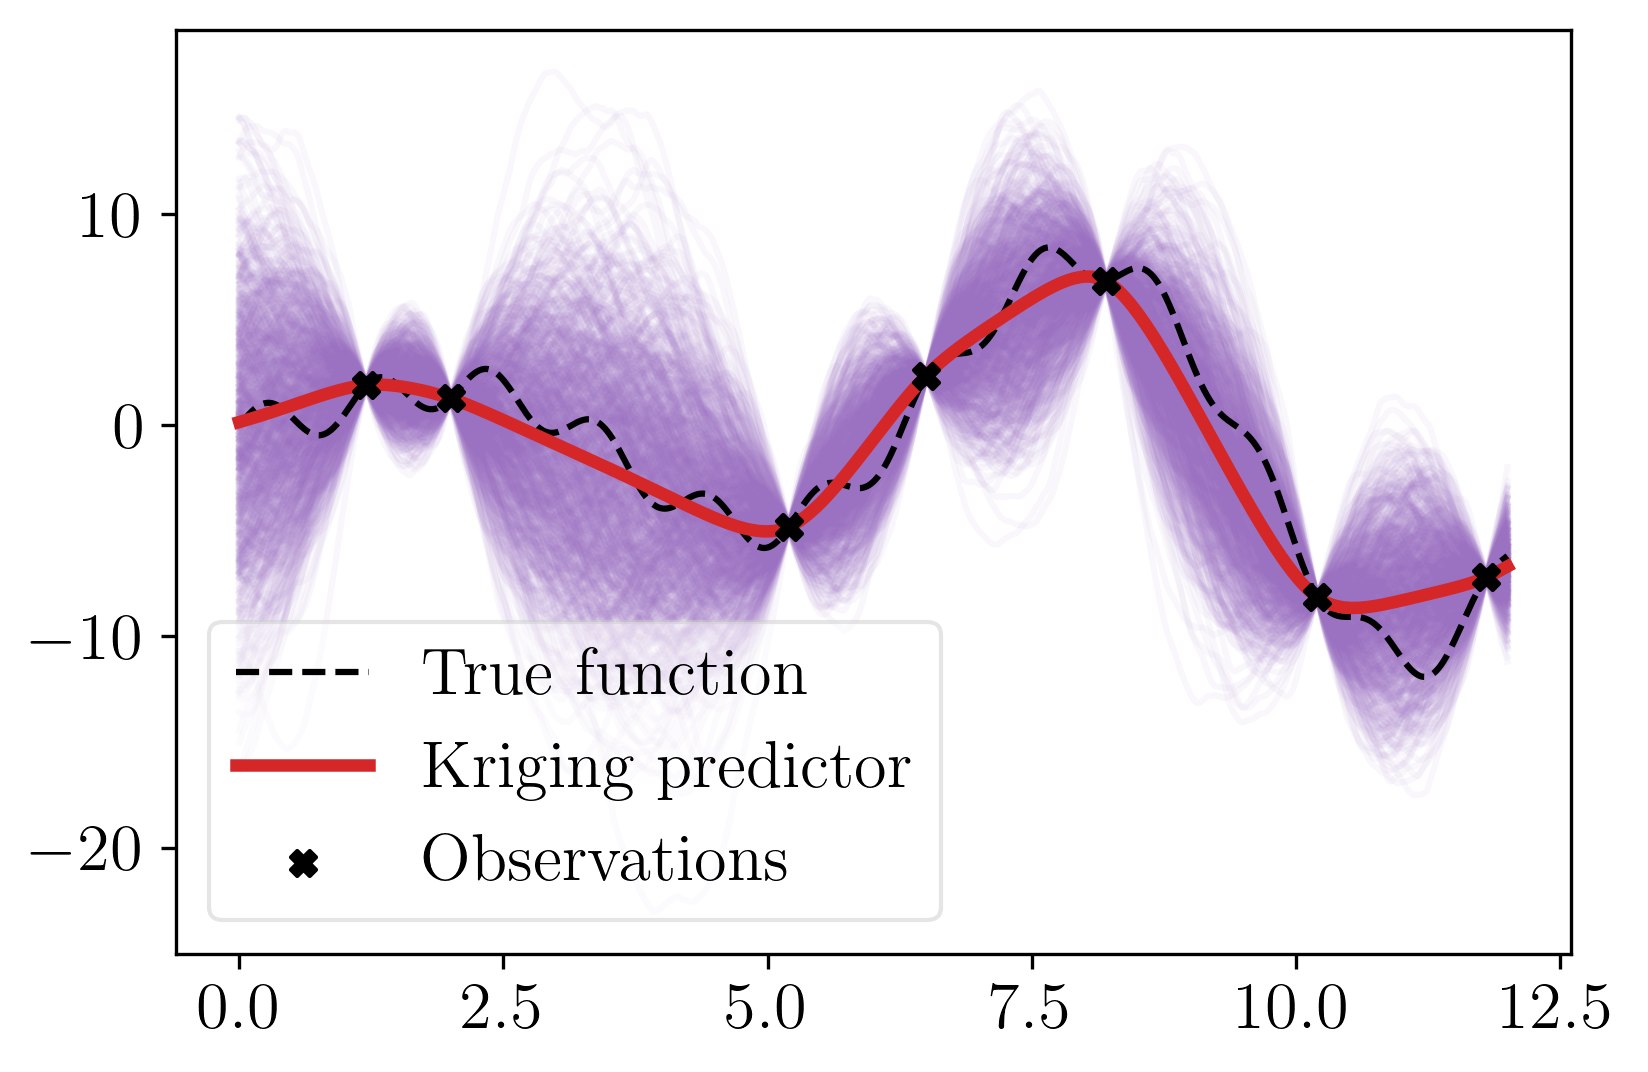
\includegraphics[width=0.6\textwidth]{../numerical_experiments/chapter1/figures/kriging_1D.png}
    \caption{Illustration of an ordinary Kriging model fitted on a limited set of observations ($n=7$). 
    The predictor is represented in and several trajectories of the conditioned GP are drawn and represented in purple.}
    \label{fig:kriging_1D}
\end{figure}


Associated with Kriging models, another validation criterion is relevant to evaluate the Kriging variance $s_n^2(\bx)$. 
The predictive variance adequation (\abv{pva}) has been introduced to confirm that the Kriging variance is reliable enough (see e.g., \citealp{bachoc_2013,demay_2022}). 
For a validation performed by holdout, and using an independent $m$-sized test set, the PVA is defined as: 
\begin{equation}
    \mathrm{PVA} = \left| \log\left( \frac1m \sum_{i=1}^{n} \frac{\left(y(\bx^{(i)}) - \wg(\bx^{(i)})\right)^2}{s_n^2(\bx^{(i)})}\right) \right|.
\end{equation}
The closer to zero this quantity gets, the better the quality of the Kriging variance. 

Despite its numerous advantages, GP regression reveals some numerical issues during the estimation of the hyperparameters, especially as the learning size increases. 
More specifically, the computation and memory allocation for the variance-covariance matrix is a recurrent issue. 
Multiple techniques solve this issue by applying compression schemes on this matrix, e.g., based on sparse approximations (e.g., hierarchical matrices as presented in \citealp{geoga_2020_hmat_gp}). 

%This section introduced a general-purpose surrogate model, uniformly approximating a function on a domain, however, surrogates are often used for specific purposes (e.g., contour finding for reliability analysis). 


%%%%%%%%%%%%%%%%%%%%%%%%%%%%%%%%%%%%%%%%%%%%%%%%%%%%%%%%%%%%%%
\begin{otexample}[\href{https://github.com/efekhari27/thesis/blob/main/numerical_experiments/chapter1/surrogates.ipynb}{Gaussian process regression}]
    A minimal working example in Python is available in Appendix~\ref{apx:D} to fit an ordinary Kriging model and active learning models. 
    Figures illustrating the present section may be reproduced, using the \ots scripts available on the GitHub repositories\footnotemark[13]\textsuperscript{,}\footnotemark[14].  
\end{otexample}
%%%%%%%%%%%%%%%%%%%%%%%%%%%%%%%%%%%%%%%%%%%%%%%%%%%%%%%%%%%%%%
\footnotetext[13]{\url{https://github.com/efekhari27/thesis/blob/main/numerical_experiments/chapter1/surrogates.ipynb}}

\footnotetext[14]{\url{https://github.com/efekhari27/thesis/blob/main/numerical_experiments/chapter1/active_learning.ipynb}}
%%%%%%%%%%%%%%%%%%%%%%%%%%%%%%%%%%%%%%%%%%%%%%%%%%%%%%%%%%%%%%


%============================================================%
\subsection{Goal-oriented active surrogate model}\label{sec:active_surrogates}
%============================================================%

Surrogates are often fitted for specific purposes, requiring an accurate approximation over a limited subdomain only. 
In these cases, a more efficient approach might be to circumscribe the learning to this subdomain. 
This approach is called a \textit{goal-oriented learning}, rather than learning uniformly over the entire domain. 
For example, to fit a surrogate model for reliability analysis, one should concentrate the learning set around the LSF. 
Similarly, to build a surrogate for a global optimization problem, one should focus the learning set around the global optimum. 
Unfortunately, the areas of interest are usually unknown before evaluating the true function. 
\textit{Active learning} is a general concept, aiming at iteratively increasing the learning set w.r.t. a \textit{learning criterion} (also called ``acquisition function''), which depends on the purpose of surrogate. 
Note that the expression ``adaptive design'' is also widely used in the computer experiments community to designate this concept.   
An exploration-exploitation trade-off arises in active learning, mostly sorted by the learning criterion.

\medskip
\begin{remark}
    This section introduces active learning methods in the computer experiment context, where the true function can be evaluated anywhere for a given computational cost. 
    However, the ``active learning'' term is also used to handle big data frameworks in the machine learning community \citep{qiu_2016}. 
    When datasets become so large that learning methods do not scale in practice, the analyst needs to select a relevant subset on which the learning is performed.  
\end{remark}
\medskip

%------------------------------------------------------------%
\subsubsection{Active Kriging for global optimization}
%------------------------------------------------------------%

In the field of black-box optimization, many methods rely on approximating the function by a surrogate. 
The use of GP as probabilistic surrogates for optimization was popularized by the \textit{efficient global optimization} (EGO) algorithm \citep{jones_1998}. 
Ever since, many related methods were developed under the generic name of \textit{Bayesian optimization}. 
The main idea is to exploit the uncertainty model from the GP to drive the selection of the next point. 
Factually, the learning criterion depends on the GP variance model.  
Numerous reviews of this field were proposed by \citet{shahriari_2015}, or \citet{gramacy_2020_book} and numerical benchmarks presented in \citet{leriche_2021}.

The generic black-box optimization problem tackled is defined as:
\begin{equation}
    \bx^* = \argmin_{\bx \in \iD_{\bX}} \, g(\bx). % \approx \argmin_{\bx \in \iD_{\bX}} \, \what{g}(\bx).
\end{equation}

To illustrate Bayesian optimization, let us present the EGO algorithm, defined by its specific learning criterion: the ``expected improvement''. 
Considering an initial learning set $\left\{\bX_n, \by_n\right\}$ built on a space-filling input design $\bX_n$ to explore the input domain. 
A first surrogate denoted by $G_n(\bx) \sim \iN(\eta_n(\bx), s_n^2(\bx))$ is fitted using \eq{eq:kriging}. 
The expected improvement (EI), to be maximized, is then written as: 
\begin{align}
    \iA^{\textrm{EI}}(\bx; \by_n) &= \E\left[\max\left(g_{\min} - G_n(\bx)\right)\right] \\ 
                                  &=\left(g_{\min} - \eta_n(\bx)\right)\, \Phi\left( \frac{g_{\min} - \eta_n(\bx)}{s_n(\bx)}\right) + 
                                    s_n(\bx) \; \phi\left(\frac{g_{\min} - \eta_n(\bx)}{s_n(\bx)}\right) \,,
    \label{eq:exp_improvement}
\end{align}
where $g_{\min} = \min(\by_n)$, $\phi$ and $\Phi$ respectively stand for the PDF and the CDF of the standard Gaussian distribution.
This learning criterion is relatively inexpensive and is used to progressively enhance the GP in order to solve the optimization problem with a limited number of calls to the true function. 

Three iterations of the EGO algorithm are represented in \fig{fig:EGO_1D} to minimize a function (dashed line), knowing a few observations (black crosses). 
After fitting an initial Kriging model (in red), the corresponding expected improvement function is represented underneath it (green line).  
This learning criterion determines the location of the observation to be added to the learning set to enhance the surrogate w.r.t. to the optimization problem. 

Bayesian optimization is an active research field, with different open problems such as constrained Bayesian optimization \citep{petit_2022}, or Bayesian optimization on stochastic functions \citep{gramacy_2020_book}. 
Similarly, active learning strategies were also adapted for structural reliability problems. 

\begin{figure}
    \centering
    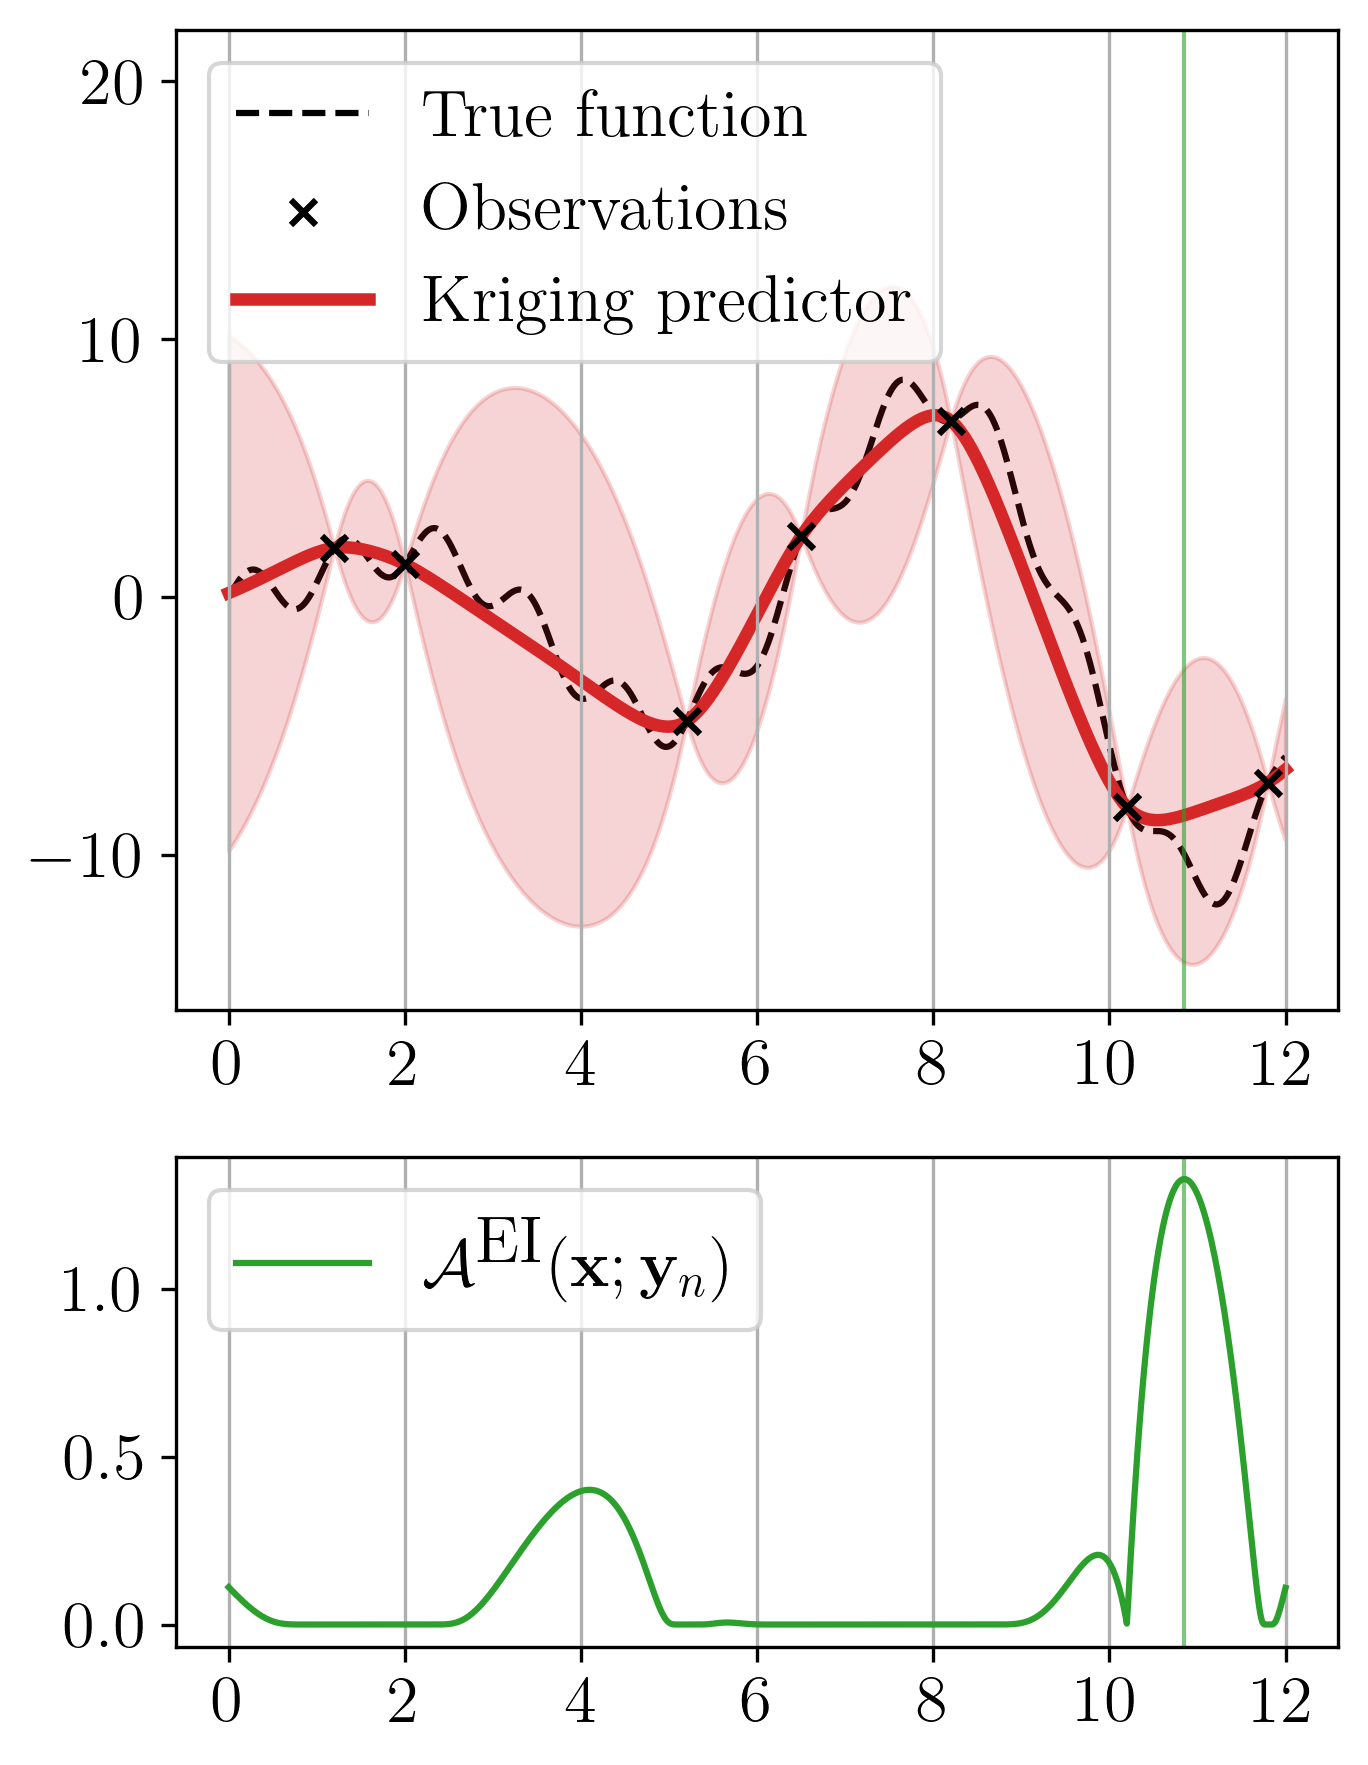
\includegraphics[width=0.32\textwidth]{../numerical_experiments/chapter1/figures/bayesian_opt_0.png}
    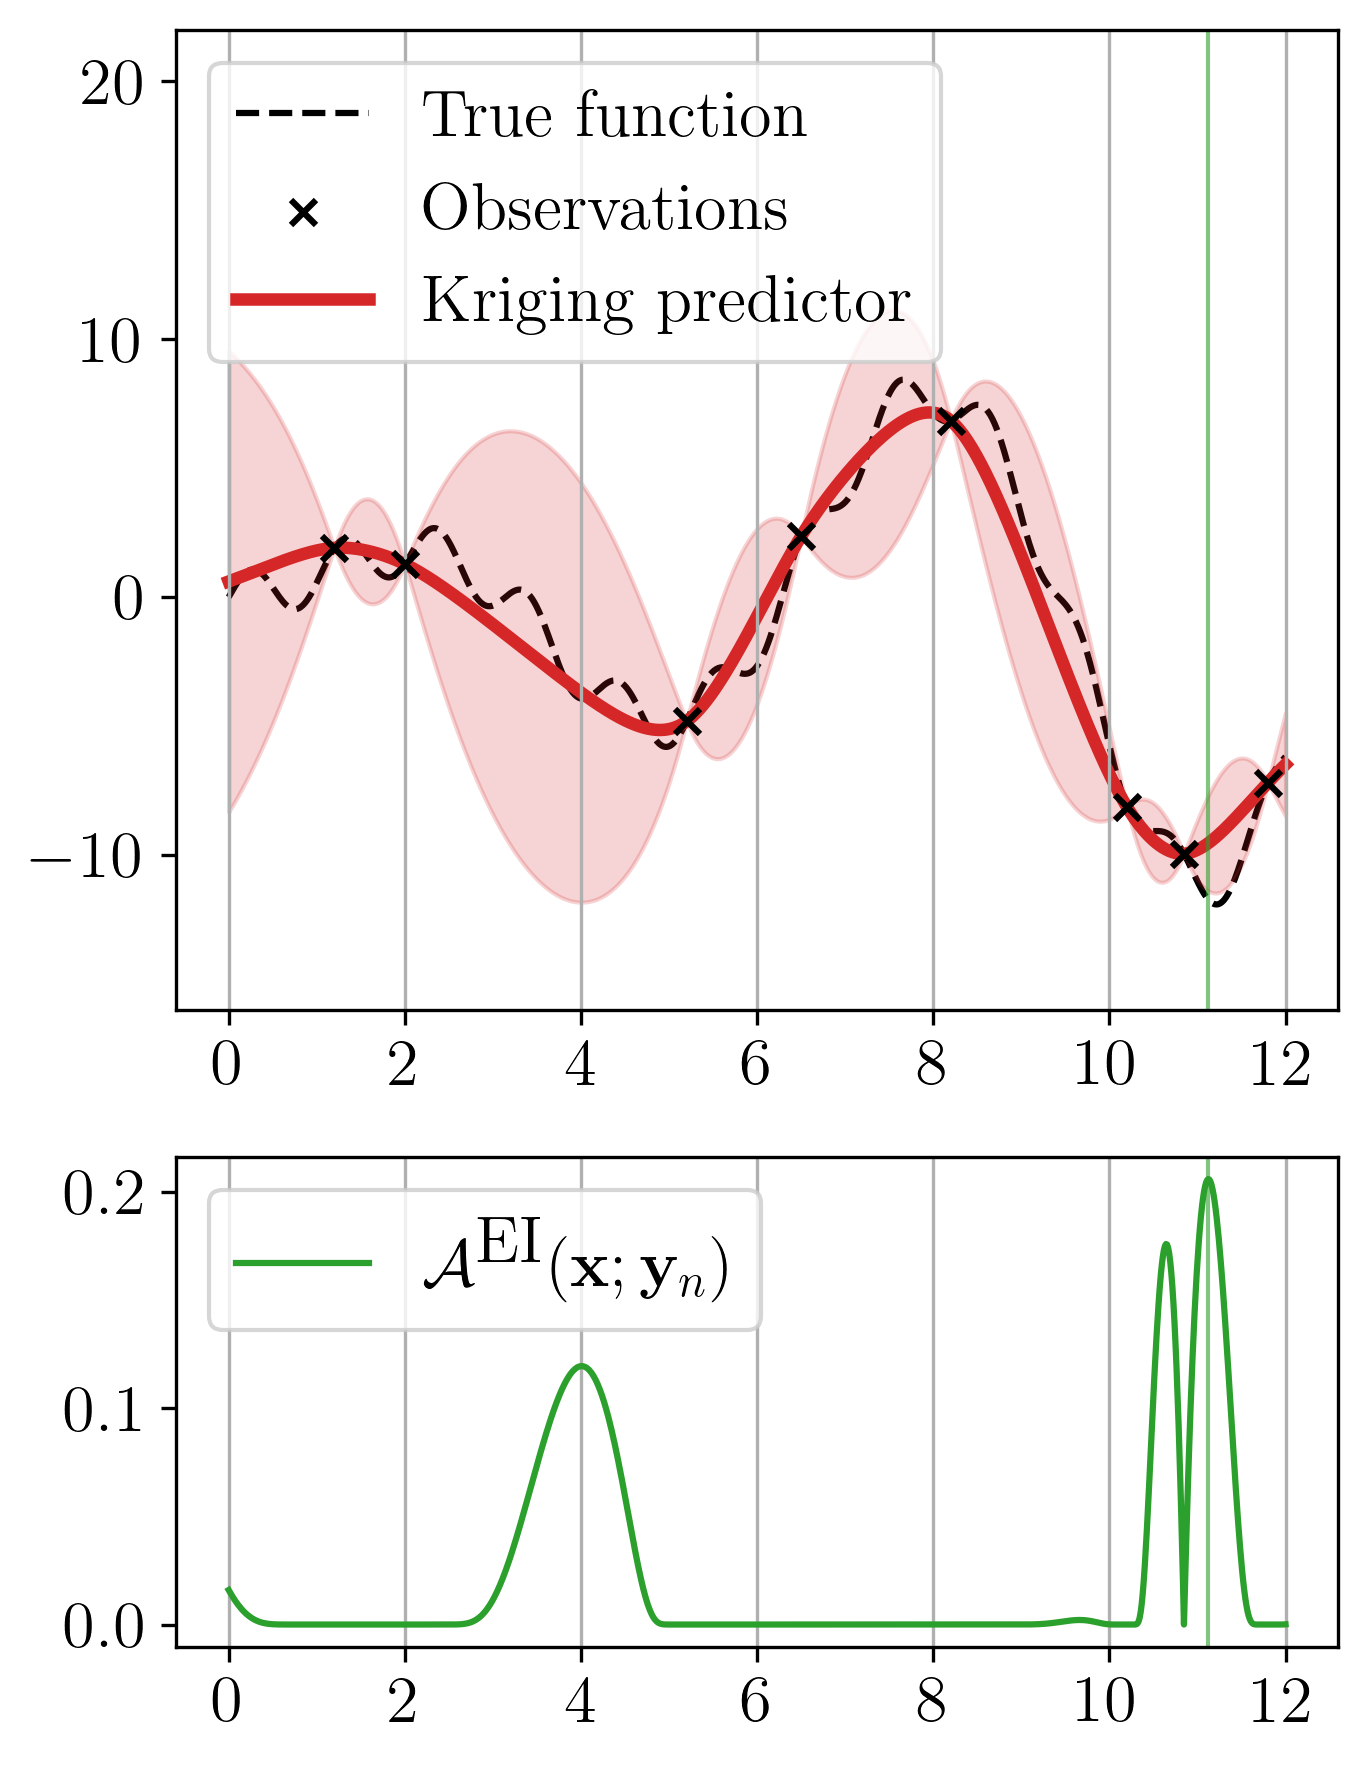
\includegraphics[width=0.32\textwidth]{../numerical_experiments/chapter1/figures/bayesian_opt_1.png}
    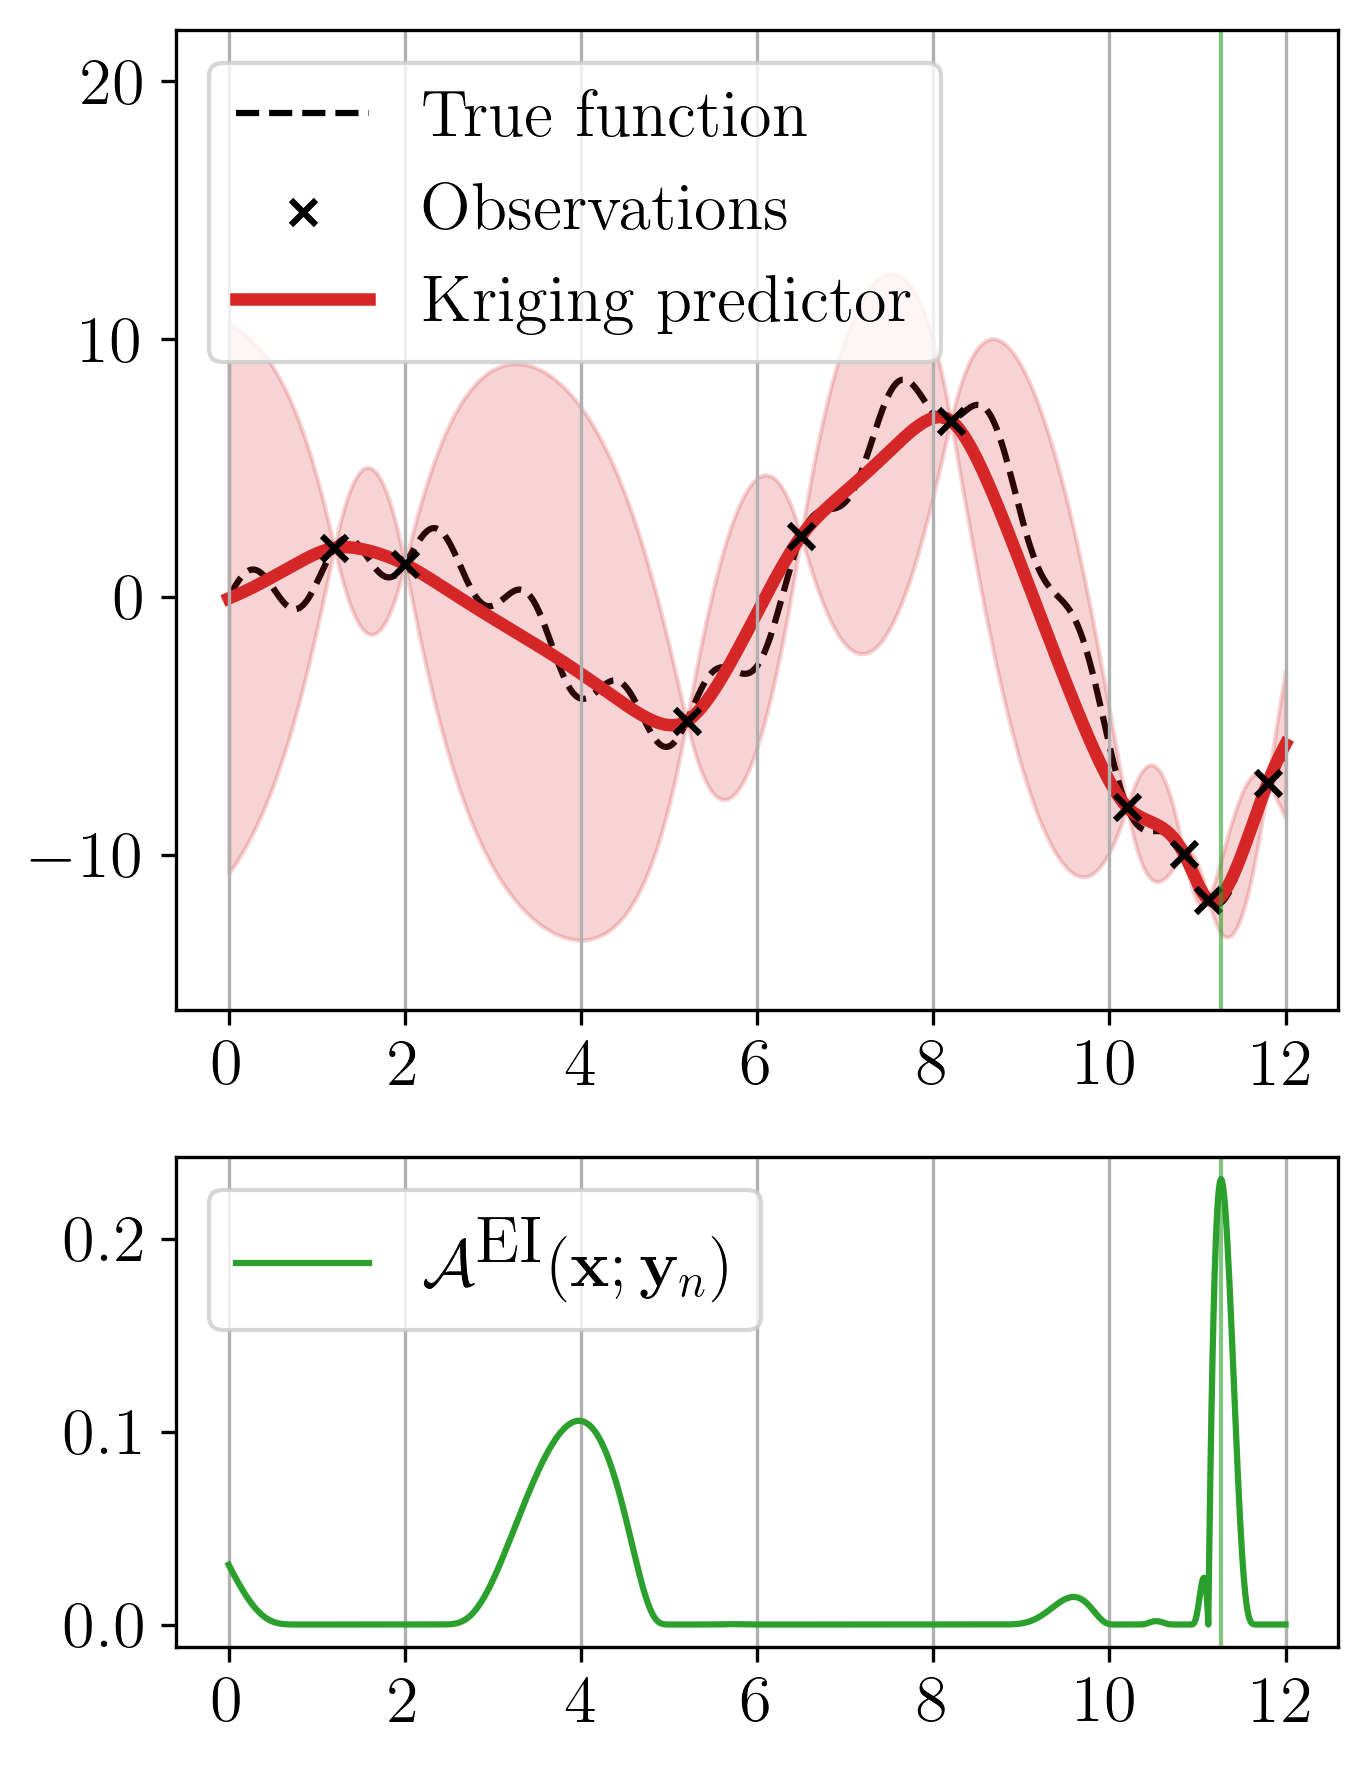
\includegraphics[width=0.32\textwidth]{../numerical_experiments/chapter1/figures/bayesian_opt_2.png}
    \caption{Illustration of the expected improvement (EI) learning criterion.}
    \label{fig:EGO_1D}
\end{figure}

%------------------------------------------------------------%
\subsubsection{Active Kriging for reliability analysis}
%------------------------------------------------------------%
Rare event estimation often requires large amounts of evaluations of the LSF (becoming intractable for costly numerical models). 
Emulating this function by a surrogate model can drastically limit the number of calls to the LSF. 
This surrogate approximates the border of the failure domain. 
However, in most cases, the failure domain represents a very restricted area of the input domain. 
Active learning methods were proposed to iteratively concentrate the learning set around this border. 

For rare event estimation, the surrogate only needs to be accurate near the LSF. 
In other words, it should accurately discriminate the points leading to the safe domain from those leading to the failure domain. 
In fact, this problem can be seen as binary classification. 
For example, active learning procedures using SVM classifiers have been adapted to this specific goal \citep{bourinet_2018}. 

The following paragraphs introduce a popular Kriging-based learning criterion called the ``deviation number'' $U$ \citep{echard_2011}, which is used in a generic algorithm named ``active Kriging'' (AK). 
The reader may refer to \citet{MorioBalesdent2015} for further active learning techniques dedicated to rare event estimation. 
More recently, \citet{teixeira_2021} and \citet{moustapha_ss_2022} reviewed this topic with the presentation of wide numerical benchmarks.

Considering an initial learning set $\left\{\bX_n, \by_n\right\}$ built on a space-filling input design $\bX_n$ to explore the domain. 
A first Gaussian process $G_n(\bx) \sim \iN(\eta_n(\bx), s_n^2(\bx))$ is fitted using \eq{eq:kriging}. 
The deviation number $U$ is looking for points close to the LSF while presenting a high Kriging variance. 
This criterion to be minimized is defined as:   
\begin{equation}
    \iA^{\textrm{U}}(\bx; \by_n) = \frac{\left|\yth - \eta_n(\bx)\right|}{s_n^2(\bx)}\, , 
    \label{eq:U}
\end{equation}
where $\yth \in R$ is a threshold defining the failure domain such as $\{\bx \in \iD_\bX \, | \, g(\bx) \leq \yth\}$. 

\fig{fig:AK_1D} reuses the same one-dimensional function as in \fig{fig:EGO_1D} to create a rare event problem. 
In this case, the failure domain is defined for output values below the threshold $\yth$. 
Here, three iterations of the active Kriging algorithm are illustrated, with the corresponding learning criterion $U$ (to minimize). 
In this simple case, the LSF is defined by the two intersections of the function with the threshold. 
Therefore, the AK method selects points near these intersections. 


Unlike optimization problems, the active methods for rare event estimation should be combined with a sampling technique. 
AK methods were coupled with most sampling techniques introduced in Section~\ref{sec:reliability} (e.g., AK-MCS, AK-IS, AK-SS). 
In practice, note that the agnostic strategy recommended after the wide benchmark of \citet{moustapha_ss_2022}, consists in coupling an AK method (using the learning function $U$) with subset simulation (taking an intermediary probability $p_0 =0.2$). 

The AK methods present the advantages of being easily implemented and interpreted, however, their learning criterion relies on a local approach. 
Alternatively, \textit{stepwise uncertainty reduction} (SUR) chooses iterative points by reducing the future expected uncertainty related to the quantity of interest \citep{bect_ginsbourger_2012}. 
If this method was proven to be theoretically more consistent \citep{bect_ginsbourger_2019}, its scaling ability is still a bottleneck.  

\begin{figure}
    \centering
    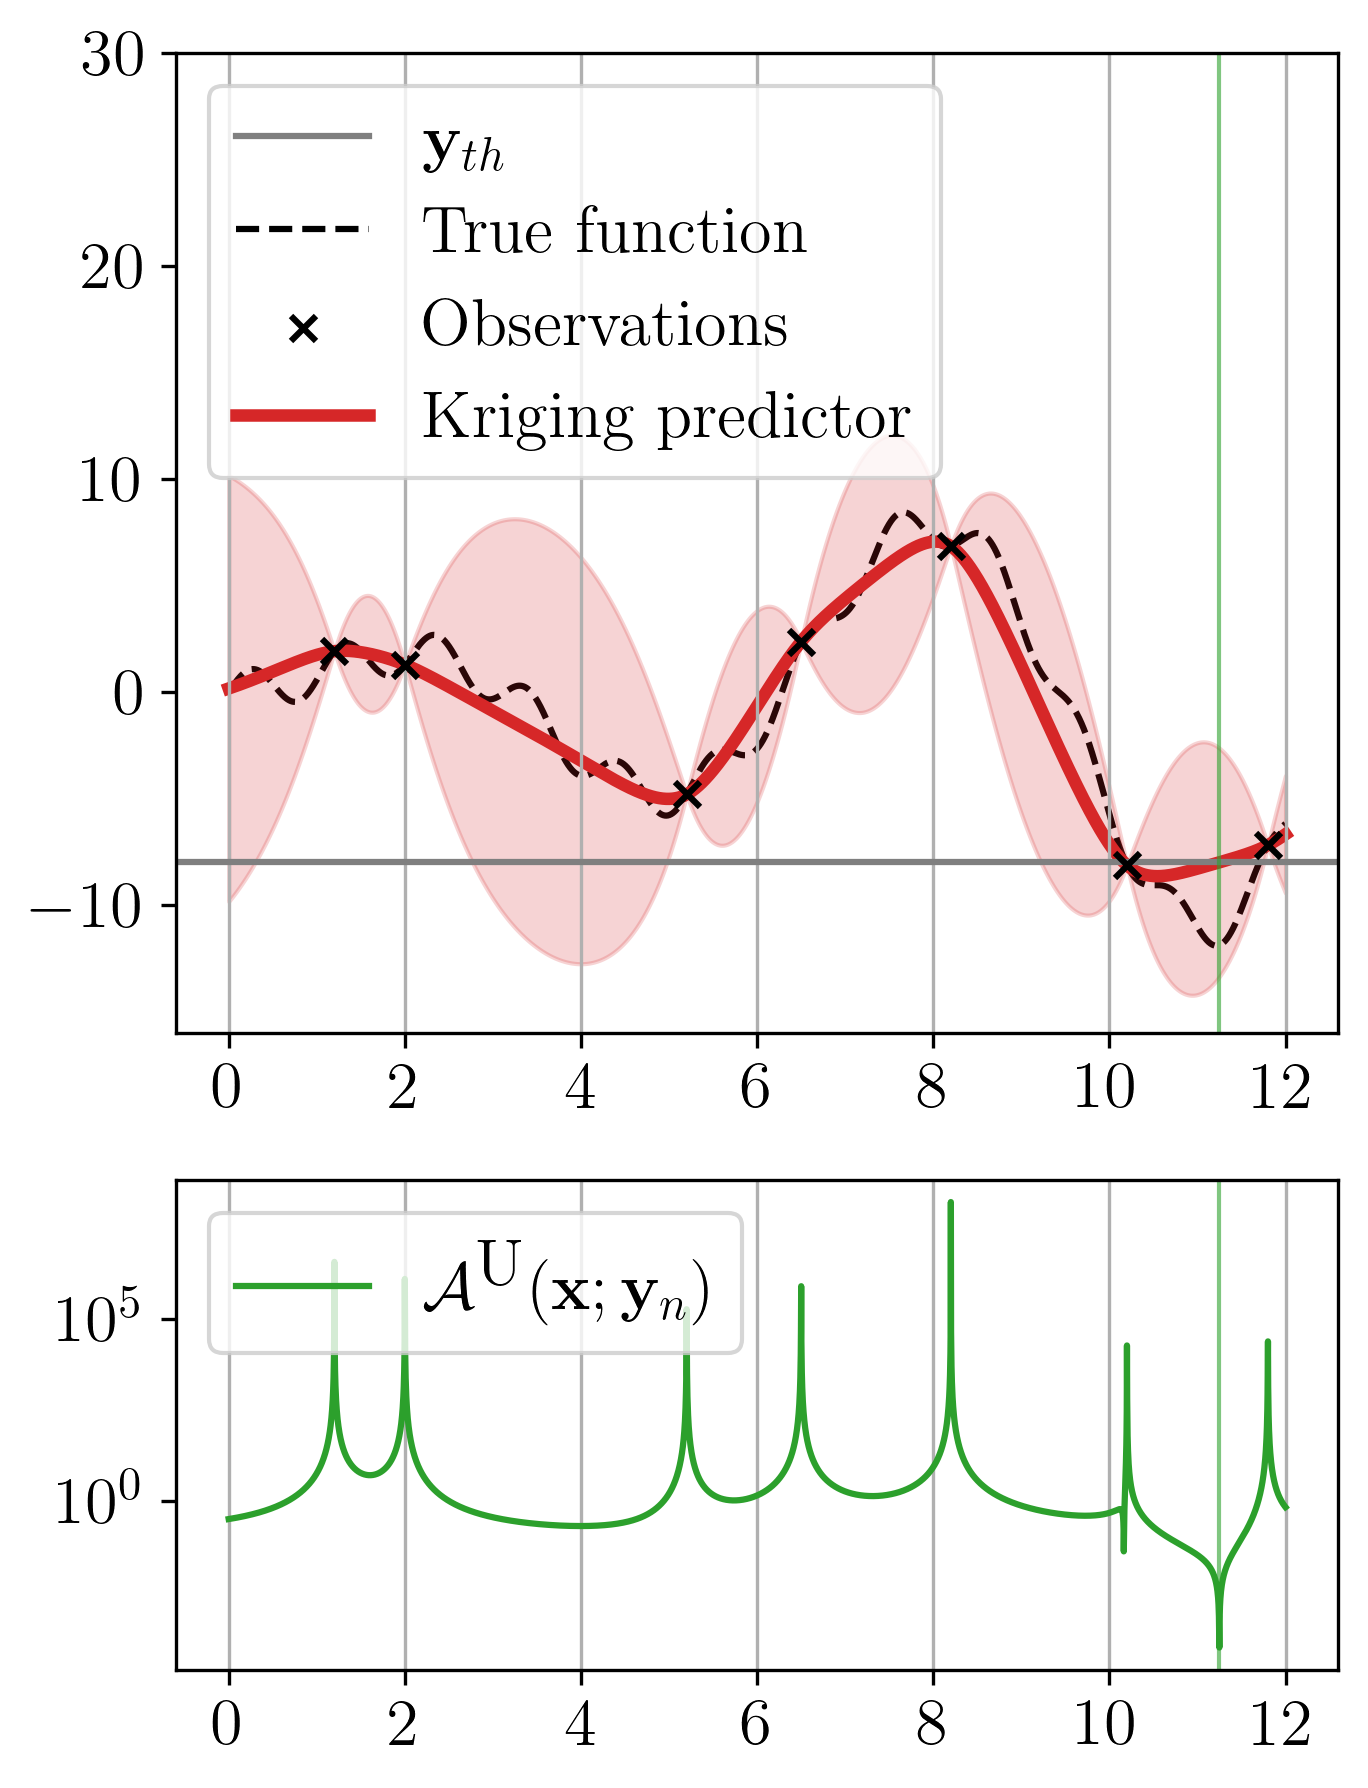
\includegraphics[width=0.32\textwidth]{../numerical_experiments/chapter1/figures/contour_find_0.png}
    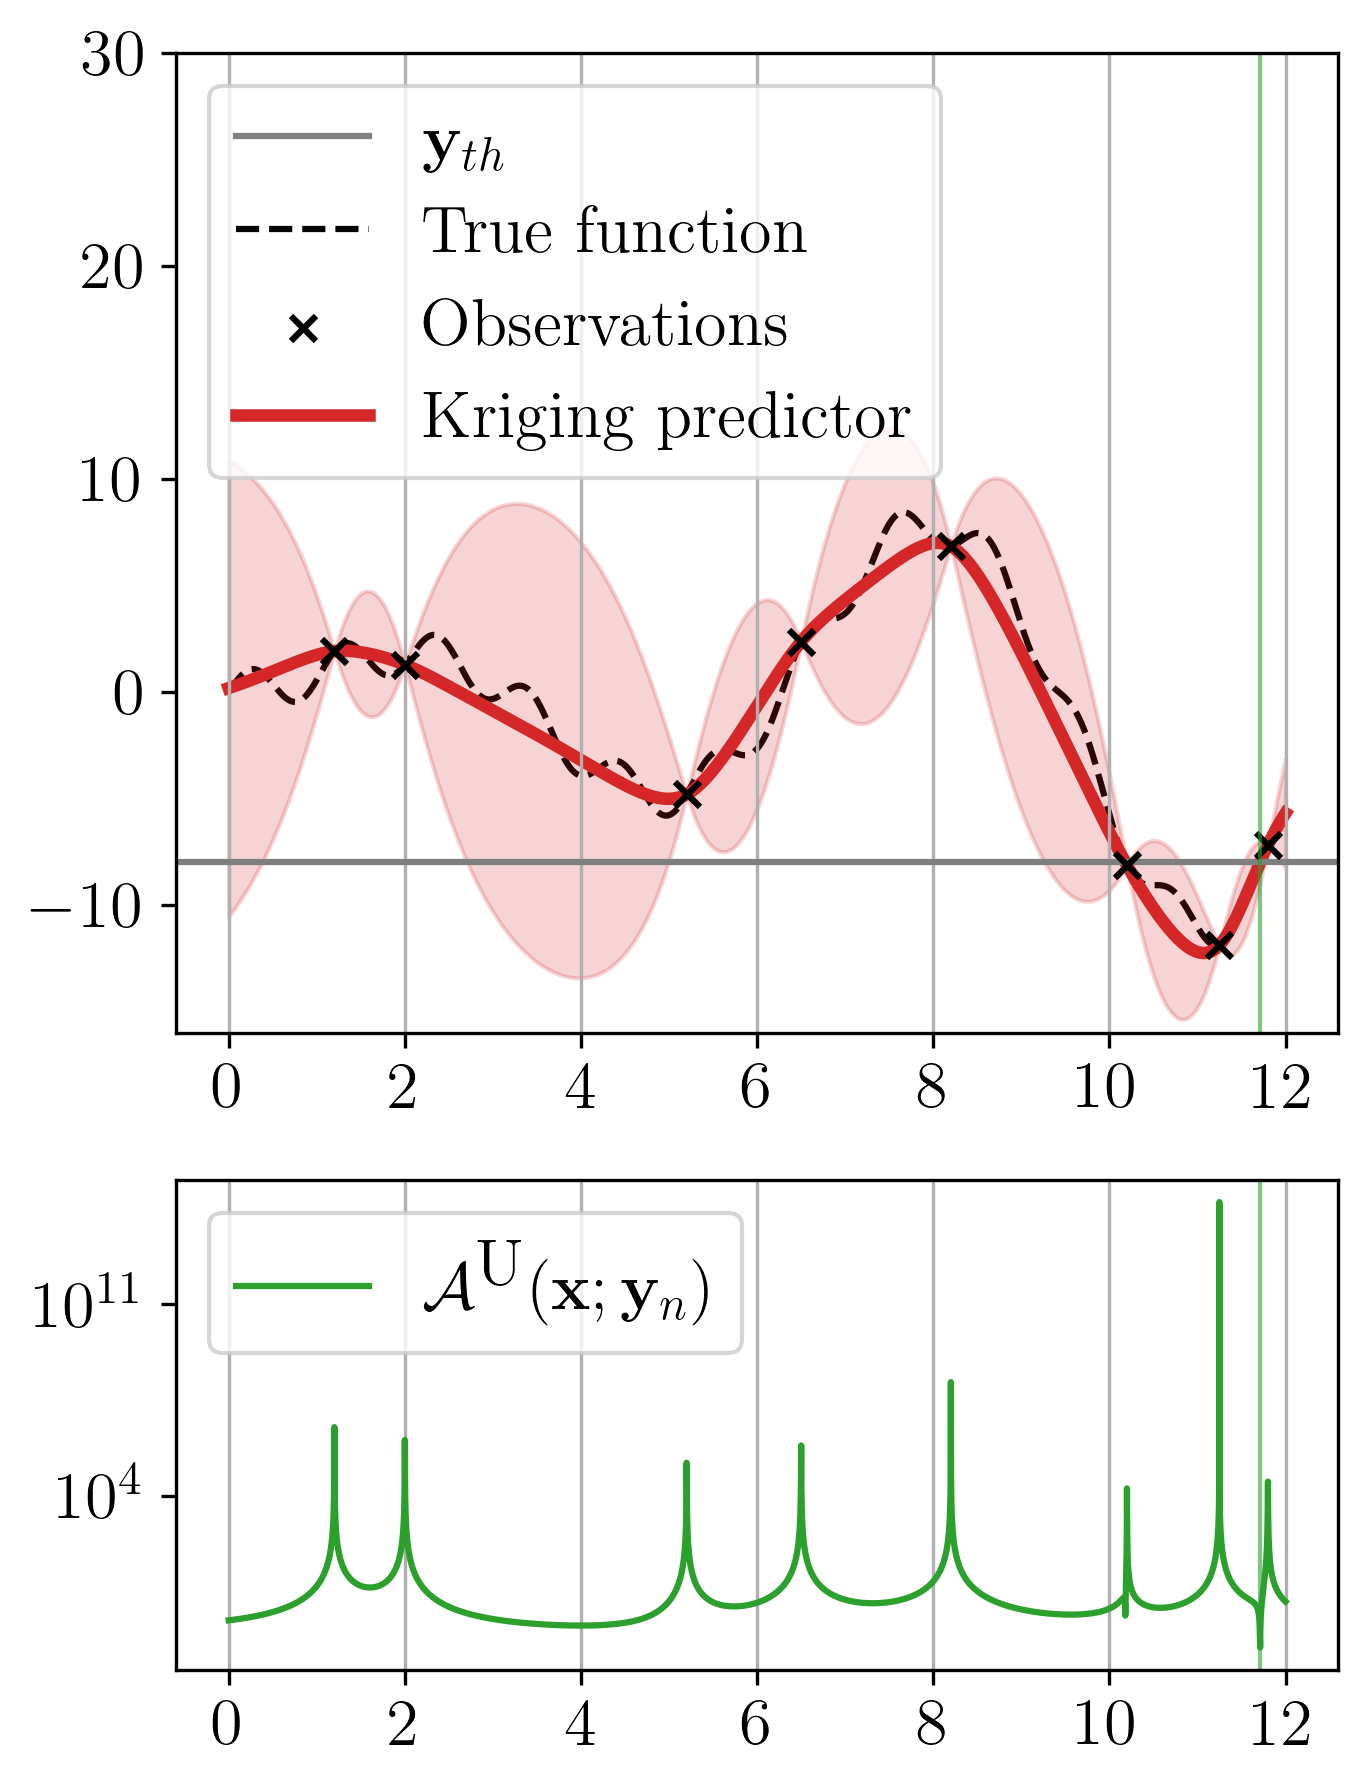
\includegraphics[width=0.32\textwidth]{../numerical_experiments/chapter1/figures/contour_find_1.png}
    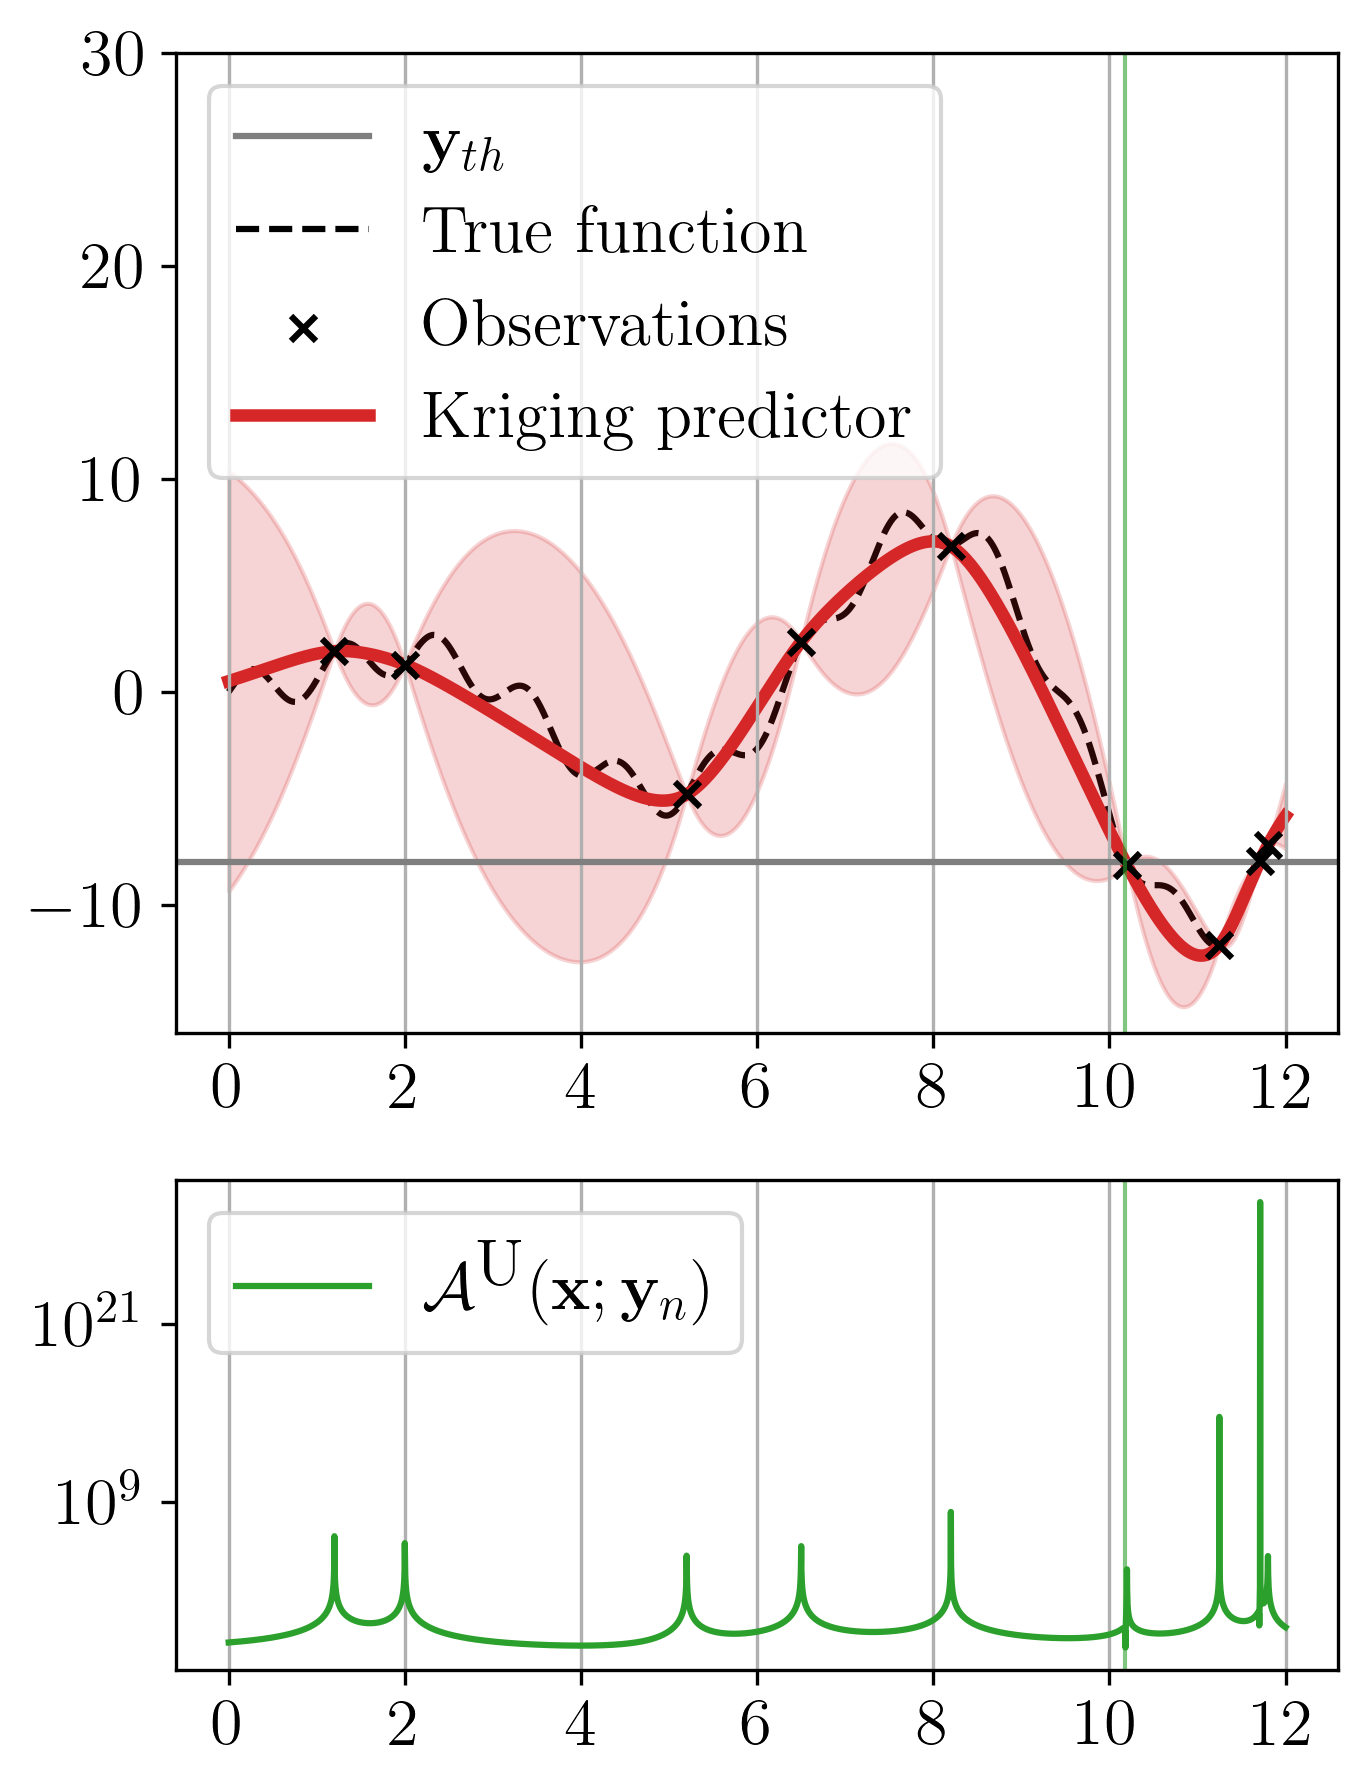
\includegraphics[width=0.32\textwidth]{../numerical_experiments/chapter1/figures/contour_find_2.png}
    \caption{Illustration of the deviation number learning criterion.}
    \label{fig:AK_1D}
\end{figure}

%============================================================%
\subsection{Summary and discussion}
%============================================================%

This section brought attention to surrogate modeling in the context of computer experiments. 
Statistical learning in this framework is made specific by the capacity of the analyst to choose the repartition of the learning set and the small data constraint (mostly due to the costly numerical models manipulated). 
In this context, many methods are used, however, Gaussian processes became popular in UQ as they consider a prior structure of uncertainty that is conditioned by observations. % (at the edge between a Bayesian and a frequentist approach). 
To enhance the learning for specific purposes (e.g., optimization or reliability analysis), active learning methods iteratively add learning points in the subdomain of interest. 
For some applications, the system studied might be modeled for different fidelities (each presenting different computational costs). 
Multi-fidelity surrogate modeling is an active field of research, associating observations from different fidelities to improve the learning \citep{fernandez_2016_review_multifi}. 
Such methods are relevant for models with a very high computational cost (typically in computer fluid dynamics).  

In UQ, surrogate models are used for uncertainty propagation (step C) and inverse analysis (step C'). 
Surrogate modeling is made difficult when the functions present discontinuities (or strong nonlinearities), high dimension, stochasticity, or nonscalar inputs or outputs. 
To deal with high dimensional problems, unimportant inputs can be screened using dedicated techniques introduced in Subsection~\ref{sec:screening}, otherwise, model order reduction methods might be used \citep{schilders_2008}. 
When the function is stochastic, several approaches allow fitting the function and its intrinsic variability \citep{binois_2019_replication,baker_2022_stochastic_surrogates_review,zhu_2023_thesis}. 

%Provided a strict validation process, surrogate models are a great opportunity for UQ. 
%However, many regulatory authorities are still reluctant to use surrogates, although their error is often much smaller than the modeling error (i.e., the error between the actual physical behavior and its numerical modeling). 


%============================================================%
%============================================================%
\section{Conclusion}
%============================================================%
%============================================================%

This section gives a literature overview of the following steps in UQ: uncertainty modeling, uncertainty propagation, global sensitivity analysis, and surrogate modeling. 
To ease the methodological presentation, all the illustrations from this section are reproducible using the Python/\ot scripts available on the GitHub repository mentioned earlier. 

Finally, the numerical models exploited are supposed to be accurate, but they obviously carry some modeling uncertainty \citep{oberkampf_2010_VVUQ}. 
In fact, prior to UQ, the model should be calibrated \citep{ghanem_2017} to make it match some physical information (e.g., measurements). 
%Numerical model calibration is also called data assimilation when a stream of measured data is available. 
%The aim of this work is to apply the tools presented in this chapter to offshore wind turbine models, therefore the next chapter introduces the numerical models manipulated in this thesis.  
